\PassOptionsToPackage{unicode=true}{hyperref} % options for packages loaded elsewhere
\PassOptionsToPackage{hyphens}{url}
%
\documentclass[]{article}
\usepackage{lmodern}
\usepackage{amssymb,amsmath}
\usepackage{ifxetex,ifluatex}
\usepackage{fixltx2e} % provides \textsubscript
\ifnum 0\ifxetex 1\fi\ifluatex 1\fi=0 % if pdftex
  \usepackage[T1]{fontenc}
  \usepackage[utf8]{inputenc}
  \usepackage{textcomp} % provides euro and other symbols
\else % if luatex or xelatex
  \usepackage{unicode-math}
  \defaultfontfeatures{Ligatures=TeX,Scale=MatchLowercase}
\fi
% use upquote if available, for straight quotes in verbatim environments
\IfFileExists{upquote.sty}{\usepackage{upquote}}{}
% use microtype if available
\IfFileExists{microtype.sty}{%
\usepackage[]{microtype}
\UseMicrotypeSet[protrusion]{basicmath} % disable protrusion for tt fonts
}{}
\IfFileExists{parskip.sty}{%
\usepackage{parskip}
}{% else
\setlength{\parindent}{0pt}
\setlength{\parskip}{6pt plus 2pt minus 1pt}
}
\usepackage{hyperref}
\hypersetup{
            pdftitle={Indonesian Samples Vs. Controls},
            pdfauthor={katalinabobowik},
            pdfborder={0 0 0},
            breaklinks=true}
\urlstyle{same}  % don't use monospace font for urls
\usepackage[margin=1in]{geometry}
\usepackage{color}
\usepackage{fancyvrb}
\newcommand{\VerbBar}{|}
\newcommand{\VERB}{\Verb[commandchars=\\\{\}]}
\DefineVerbatimEnvironment{Highlighting}{Verbatim}{commandchars=\\\{\}}
% Add ',fontsize=\small' for more characters per line
\usepackage{framed}
\definecolor{shadecolor}{RGB}{248,248,248}
\newenvironment{Shaded}{\begin{snugshade}}{\end{snugshade}}
\newcommand{\AlertTok}[1]{\textcolor[rgb]{0.94,0.16,0.16}{#1}}
\newcommand{\AnnotationTok}[1]{\textcolor[rgb]{0.56,0.35,0.01}{\textbf{\textit{#1}}}}
\newcommand{\AttributeTok}[1]{\textcolor[rgb]{0.77,0.63,0.00}{#1}}
\newcommand{\BaseNTok}[1]{\textcolor[rgb]{0.00,0.00,0.81}{#1}}
\newcommand{\BuiltInTok}[1]{#1}
\newcommand{\CharTok}[1]{\textcolor[rgb]{0.31,0.60,0.02}{#1}}
\newcommand{\CommentTok}[1]{\textcolor[rgb]{0.56,0.35,0.01}{\textit{#1}}}
\newcommand{\CommentVarTok}[1]{\textcolor[rgb]{0.56,0.35,0.01}{\textbf{\textit{#1}}}}
\newcommand{\ConstantTok}[1]{\textcolor[rgb]{0.00,0.00,0.00}{#1}}
\newcommand{\ControlFlowTok}[1]{\textcolor[rgb]{0.13,0.29,0.53}{\textbf{#1}}}
\newcommand{\DataTypeTok}[1]{\textcolor[rgb]{0.13,0.29,0.53}{#1}}
\newcommand{\DecValTok}[1]{\textcolor[rgb]{0.00,0.00,0.81}{#1}}
\newcommand{\DocumentationTok}[1]{\textcolor[rgb]{0.56,0.35,0.01}{\textbf{\textit{#1}}}}
\newcommand{\ErrorTok}[1]{\textcolor[rgb]{0.64,0.00,0.00}{\textbf{#1}}}
\newcommand{\ExtensionTok}[1]{#1}
\newcommand{\FloatTok}[1]{\textcolor[rgb]{0.00,0.00,0.81}{#1}}
\newcommand{\FunctionTok}[1]{\textcolor[rgb]{0.00,0.00,0.00}{#1}}
\newcommand{\ImportTok}[1]{#1}
\newcommand{\InformationTok}[1]{\textcolor[rgb]{0.56,0.35,0.01}{\textbf{\textit{#1}}}}
\newcommand{\KeywordTok}[1]{\textcolor[rgb]{0.13,0.29,0.53}{\textbf{#1}}}
\newcommand{\NormalTok}[1]{#1}
\newcommand{\OperatorTok}[1]{\textcolor[rgb]{0.81,0.36,0.00}{\textbf{#1}}}
\newcommand{\OtherTok}[1]{\textcolor[rgb]{0.56,0.35,0.01}{#1}}
\newcommand{\PreprocessorTok}[1]{\textcolor[rgb]{0.56,0.35,0.01}{\textit{#1}}}
\newcommand{\RegionMarkerTok}[1]{#1}
\newcommand{\SpecialCharTok}[1]{\textcolor[rgb]{0.00,0.00,0.00}{#1}}
\newcommand{\SpecialStringTok}[1]{\textcolor[rgb]{0.31,0.60,0.02}{#1}}
\newcommand{\StringTok}[1]{\textcolor[rgb]{0.31,0.60,0.02}{#1}}
\newcommand{\VariableTok}[1]{\textcolor[rgb]{0.00,0.00,0.00}{#1}}
\newcommand{\VerbatimStringTok}[1]{\textcolor[rgb]{0.31,0.60,0.02}{#1}}
\newcommand{\WarningTok}[1]{\textcolor[rgb]{0.56,0.35,0.01}{\textbf{\textit{#1}}}}
\usepackage{graphicx,grffile}
\makeatletter
\def\maxwidth{\ifdim\Gin@nat@width>\linewidth\linewidth\else\Gin@nat@width\fi}
\def\maxheight{\ifdim\Gin@nat@height>\textheight\textheight\else\Gin@nat@height\fi}
\makeatother
% Scale images if necessary, so that they will not overflow the page
% margins by default, and it is still possible to overwrite the defaults
% using explicit options in \includegraphics[width, height, ...]{}
\setkeys{Gin}{width=\maxwidth,height=\maxheight,keepaspectratio}
\setlength{\emergencystretch}{3em}  % prevent overfull lines
\providecommand{\tightlist}{%
  \setlength{\itemsep}{0pt}\setlength{\parskip}{0pt}}
\setcounter{secnumdepth}{0}
% Redefines (sub)paragraphs to behave more like sections
\ifx\paragraph\undefined\else
\let\oldparagraph\paragraph
\renewcommand{\paragraph}[1]{\oldparagraph{#1}\mbox{}}
\fi
\ifx\subparagraph\undefined\else
\let\oldsubparagraph\subparagraph
\renewcommand{\subparagraph}[1]{\oldsubparagraph{#1}\mbox{}}
\fi

% set default figure placement to htbp
\makeatletter
\def\fps@figure{htbp}
\makeatother


\title{Indonesian Samples Vs. Controls}
\author{katalinabobowik}
\date{2020-09-13}

\begin{document}
\maketitle

Last updated: 2020-10-13

\hypertarget{introduction}{%
\section{Introduction}\label{introduction}}

This part of the study will analyse differences between our Indonesian
samples and compare them with healthy controls. From my previous
analysis of healthy Indonesians, I found that Plasmodium, Flavivirus,
and Bacteria make up the majority of the taxa found within unmapped
reads. However, I want to see how different this is to populations in
more sterile environments.

The aim of this analysis is therefore to test whether the pathogen
signature identified in our Indonesian samples is unique. We will test
this by looking at the sample grouping by PCA, hierarchical clustering,
relative abundance of taxa, alpha and beta diversity estimates, and
differential abundance testing.

The Indonesian data in this study were generated from the
previously-published study by
\href{https://journals.plos.org/plosgenetics/article?id=10.1371/journal.pgen.1008749}{Natri
et al}. Briefly, 101-bp, paired-end data were generated on an Illumina
HiSeq 2500 to an average depth of 30 million read pairs per
individualon.

it was run through KMA, CCMetage, etc\ldots{} (look at scripts, x, y, z,
for sample processing)

The control samples were taken from Loohuis et al.

These two other studies are\ldots{}

\hypertarget{loading-packages-and-colour-setup}{%
\section{Loading packages and colour
setup}\label{loading-packages-and-colour-setup}}

The code below will install the packages needed to run the analyses.
We're also setting up our directories to run locally, but I've provided
all of the paths so they can be easily modified if they need to be run
on the server.

\begin{Shaded}
\begin{Highlighting}[]
\KeywordTok{require}\NormalTok{(ggplot2)}
\KeywordTok{require}\NormalTok{(RColorBrewer)}
\KeywordTok{library}\NormalTok{(dplyr)}
\KeywordTok{library}\NormalTok{(plyr)}
\KeywordTok{library}\NormalTok{(reshape2)}
\KeywordTok{library}\NormalTok{(ggpubr)}
\KeywordTok{library}\NormalTok{(metacoder)}
\KeywordTok{library}\NormalTok{(tidyverse)             }
\KeywordTok{library}\NormalTok{(phyloseq)                   }
\KeywordTok{library}\NormalTok{(DESeq2)                       }
\KeywordTok{library}\NormalTok{(microbiome)               }
\KeywordTok{library}\NormalTok{(vegan)                         }
\KeywordTok{library}\NormalTok{(picante)                     }
\KeywordTok{library}\NormalTok{(ALDEx2)                      }
\KeywordTok{library}\NormalTok{(metagenomeSeq)          }
\KeywordTok{library}\NormalTok{(HMP)                             }
\KeywordTok{library}\NormalTok{(dendextend)               }
\KeywordTok{library}\NormalTok{(selbal)                       }
\KeywordTok{library}\NormalTok{(rms)}
\KeywordTok{library}\NormalTok{(breakaway)        }
\KeywordTok{library}\NormalTok{(microbiomeutilities)}
\KeywordTok{library}\NormalTok{(mixOmics)}
\KeywordTok{library}\NormalTok{(SRS)}
\KeywordTok{library}\NormalTok{(ggrepel)}

\CommentTok{# set up directories}
\NormalTok{refdir =}\StringTok{ "/Users/katalinabobowik/Documents/UniMelb_PhD/Analysis/UniMelb_Sumba/ReferenceFiles/EpiStudy/"}
\NormalTok{filteringDir =}\StringTok{ "/Users/katalinabobowik/Documents/UniMelb_PhD/Analysis/UniMelb_Sumba/Output/Epi_Study/ControlSampleComparison/"}
\end{Highlighting}
\end{Shaded}

We'll also set up our colour schemes.

\begin{Shaded}
\begin{Highlighting}[]
\CommentTok{# set ggplot colour theme to white}
\KeywordTok{theme_set}\NormalTok{(}\KeywordTok{theme_bw}\NormalTok{())}

\CommentTok{# Set up colour scheme}
\NormalTok{IndonesiaCol=}\StringTok{"#4477AA"}
\NormalTok{MaliCol=}\StringTok{"#228833"}
\NormalTok{UKCol=}\StringTok{"#AA3377"}
\end{Highlighting}
\end{Shaded}

\hypertarget{reading-in-the-indonesian-data}{%
\section{Reading in the Indonesian
data}\label{reading-in-the-indonesian-data}}

Many microbiome studies use the package phyloseq to analyse data due to
its comprehensive packages. The data structures in Phyloseq (taxa data,
otu data, and sample data) are also contained in a single object, which
makes it easy to keep everything together.

First, we'll read in our Indonesian single-ended count data and separate
taxa information from read abundance information. We'll then assign
sample information to the data (namely, population and sample IDs) so
that we can compare it to the control datasets.

\begin{Shaded}
\begin{Highlighting}[]
\NormalTok{AllREadsSE_Indo_Counts <-}\StringTok{ }\KeywordTok{read.csv}\NormalTok{(}\KeywordTok{paste0}\NormalTok{(refdir,}\StringTok{"Counts_Indo_75BP_SE.csv"}\NormalTok{),}\DataTypeTok{check.names=}\OtherTok{FALSE}\NormalTok{)}

\CommentTok{# Separate species' abundances and taxonomy columns}
\NormalTok{taxa_raw <-}\StringTok{ }\KeywordTok{as.matrix}\NormalTok{(AllREadsSE_Indo_Counts[,}\KeywordTok{c}\NormalTok{(}\StringTok{"Superkingdom"}\NormalTok{,}\StringTok{"Kingdom"}\NormalTok{,}\StringTok{"Phylum"}\NormalTok{, }\StringTok{"Class"}\NormalTok{, }\StringTok{"Order"}\NormalTok{,}\StringTok{"Family"}\NormalTok{,}\StringTok{"Genus"}\NormalTok{,}\StringTok{"Species"}\NormalTok{)])}
\NormalTok{abund_raw <-}\StringTok{ }\KeywordTok{as.matrix}\NormalTok{(AllREadsSE_Indo_Counts[,}\OperatorTok{-}\KeywordTok{which}\NormalTok{(}\KeywordTok{colnames}\NormalTok{(AllREadsSE_Indo_Counts) }\OperatorTok\StringTok{ }\KeywordTok{c}\NormalTok{(}\StringTok{"Superkingdom"}\NormalTok{,}\StringTok{"Kingdom"}\NormalTok{,}\StringTok{"Phylum"}\NormalTok{, }\StringTok{"Class"}\NormalTok{, }\StringTok{"Order"}\NormalTok{,}\StringTok{"Family"}\NormalTok{,}\StringTok{"Genus"}\NormalTok{,}\StringTok{"Species"}\NormalTok{))])}

\CommentTok{# convert to Phyloseq object}
\NormalTok{tax =}\StringTok{ }\KeywordTok{tax_table}\NormalTok{(taxa_raw)}
\NormalTok{taxa =}\StringTok{ }\KeywordTok{otu_table}\NormalTok{(abund_raw, }\DataTypeTok{taxa_are_rows =} \OtherTok{TRUE}\NormalTok{)}
\NormalTok{AllREadsSE_Indo_Counts_physeq =}\StringTok{ }\KeywordTok{phyloseq}\NormalTok{(taxa, tax)}

\CommentTok{# add in sample information, starting with Island}
\NormalTok{samplenames <-}\StringTok{ }\KeywordTok{colnames}\NormalTok{(}\KeywordTok{otu_table}\NormalTok{(AllREadsSE_Indo_Counts_physeq))}
\NormalTok{pop <-}\StringTok{ }\KeywordTok{rep}\NormalTok{(}\StringTok{"Indonesia"}\NormalTok{,}\KeywordTok{ncol}\NormalTok{(}\KeywordTok{otu_table}\NormalTok{(AllREadsSE_Indo_Counts_physeq)))}

\CommentTok{# make this into a df and add to the Phloseq object}
\NormalTok{samples_df=}\KeywordTok{data.frame}\NormalTok{(}\DataTypeTok{SampleName=}\KeywordTok{colnames}\NormalTok{(}\KeywordTok{otu_table}\NormalTok{(AllREadsSE_Indo_Counts_physeq)), }\DataTypeTok{SamplePop=}\NormalTok{pop)}
\NormalTok{samples =}\StringTok{ }\KeywordTok{sample_data}\NormalTok{(samples_df)}
\KeywordTok{rownames}\NormalTok{(samples)=samples}\OperatorTok{$}\NormalTok{SampleName}
\KeywordTok{sample_data}\NormalTok{(AllREadsSE_Indo_Counts_physeq) <-}\StringTok{ }\NormalTok{samples}

\CommentTok{# get information on phyloseq objects}
\NormalTok{AllREadsSE_Indo_Counts_physeq}
\end{Highlighting}
\end{Shaded}

\begin{verbatim}
## phyloseq-class experiment-level object
## otu_table()   OTU Table:         [ 2458 taxa and 123 samples ]
## sample_data() Sample Data:       [ 123 samples by 2 sample variables ]
## tax_table()   Taxonomy Table:    [ 2458 taxa by 8 taxonomic ranks ]
\end{verbatim}

For the Indonesian samples, we can see that we have a phyloseq object
consisting of 123 samples, 6 of which are replicates. We'll take the
replicates with the highest library depth and then remove the rest.

\begin{Shaded}
\begin{Highlighting}[]
\CommentTok{# get replicates}
\NormalTok{trimmed_samplenames =}\StringTok{ }\KeywordTok{gsub}\NormalTok{(}\StringTok{"Batch1"}\NormalTok{,}\StringTok{''}\NormalTok{,samplenames) }\OperatorTok\StringTok{ }\KeywordTok{gsub}\NormalTok{(}\StringTok{"Batch2"}\NormalTok{,}\StringTok{''}\NormalTok{, .) }\OperatorTok\StringTok{ }\KeywordTok{gsub}\NormalTok{(}\StringTok{"Batch3"}\NormalTok{,}\StringTok{''}\NormalTok{, .)}
\NormalTok{trimmed_samplenames =}\StringTok{ }\KeywordTok{sub}\NormalTok{(}\StringTok{"([A-Z]\{3\})([0-9]\{3\})"}\NormalTok{, }\StringTok{"}\CharTok{\textbackslash{}\textbackslash{}}\StringTok{1-}\CharTok{\textbackslash{}\textbackslash{}}\StringTok{2"}\NormalTok{, trimmed_samplenames)}
\NormalTok{replicate_index =}\StringTok{ }\KeywordTok{which}\NormalTok{(}\KeywordTok{duplicated}\NormalTok{(trimmed_samplenames) }\OperatorTok{|}\StringTok{ }\KeywordTok{duplicated}\NormalTok{(trimmed_samplenames, }\DataTypeTok{fromLast =} \OtherTok{TRUE}\NormalTok{))}
\NormalTok{replicates =}\StringTok{ }\NormalTok{samplenames[replicate_index]}

\CommentTok{# add sequencing depth information to the Physeq object in order to filter replicates by seqDepth}
\NormalTok{SeqDepth =}\StringTok{ }\KeywordTok{colSums}\NormalTok{(}\KeywordTok{otu_table}\NormalTok{(AllREadsSE_Indo_Counts_physeq))}
\KeywordTok{sample_data}\NormalTok{(AllREadsSE_Indo_Counts_physeq)}\OperatorTok{$}\NormalTok{SeqDepth =}\StringTok{ }\NormalTok{SeqDepth}

\CommentTok{# find out which replicates have the highest sequencing depth}
\KeywordTok{sample_data}\NormalTok{(AllREadsSE_Indo_Counts_physeq)[replicates,]}
\end{Highlighting}
\end{Shaded}

\begin{verbatim}
##                          SampleName SamplePop SeqDepth
## MPI-381Batch1         MPI-381Batch1 Indonesia    31097
## MPI-381Batch3         MPI-381Batch3 Indonesia    35468
## MTW-TLL-013Batch2 MTW-TLL-013Batch2 Indonesia    42231
## MTW-TLL013Batch3   MTW-TLL013Batch3 Indonesia    37580
## SMB-ANK-016Batch2 SMB-ANK-016Batch2 Indonesia   111419
## SMB-ANK-027Batch1 SMB-ANK-027Batch1 Indonesia    39086
## SMB-ANK-027Batch2 SMB-ANK-027Batch2 Indonesia    46355
## SMB-ANK016Batch3   SMB-ANK016Batch3 Indonesia    27387
## SMB-ANK027Batch3   SMB-ANK027Batch3 Indonesia    48014
## SMB-WNG-021Batch1 SMB-WNG-021Batch1 Indonesia    53616
## SMB-WNG021Batch3   SMB-WNG021Batch3 Indonesia    35954
\end{verbatim}

\begin{Shaded}
\begin{Highlighting}[]
\NormalTok{replicateDF=}\KeywordTok{as.data.frame}\NormalTok{(}\KeywordTok{sample_data}\NormalTok{(AllREadsSE_Indo_Counts_physeq)[replicates,])}
\NormalTok{replicateDF}\OperatorTok{$}\NormalTok{SampleName =}\StringTok{ }\KeywordTok{sub}\NormalTok{(}\StringTok{"([A-Z]\{3\})([0-9]\{3\})"}\NormalTok{, }\StringTok{"}\CharTok{\textbackslash{}\textbackslash{}}\StringTok{1-}\CharTok{\textbackslash{}\textbackslash{}}\StringTok{2"}\NormalTok{, replicateDF}\OperatorTok{$}\NormalTok{SampleName)}
\NormalTok{replicateDF}\OperatorTok{$}\NormalTok{SampleName =}\StringTok{ }\KeywordTok{gsub}\NormalTok{(}\StringTok{"Batch1"}\NormalTok{,}\StringTok{''}\NormalTok{,replicateDF}\OperatorTok{$}\NormalTok{SampleName) }\OperatorTok\StringTok{ }\KeywordTok{gsub}\NormalTok{(}\StringTok{"Batch2"}\NormalTok{,}\StringTok{''}\NormalTok{, .) }\OperatorTok\StringTok{ }\KeywordTok{gsub}\NormalTok{(}\StringTok{"Batch3"}\NormalTok{,}\StringTok{''}\NormalTok{, .)}
\NormalTok{replicateDF=replicateDF[}\KeywordTok{with}\NormalTok{(replicateDF, }\KeywordTok{order}\NormalTok{(}\OperatorTok{-}\NormalTok{SeqDepth)), ]}
\NormalTok{removeReplicates=}\KeywordTok{rownames}\NormalTok{(replicateDF[}\KeywordTok{which}\NormalTok{(}\KeywordTok{duplicated}\NormalTok{(replicateDF}\OperatorTok{$}\NormalTok{SampleName)),])}
\NormalTok{keepReplicates=}\KeywordTok{rownames}\NormalTok{(}\KeywordTok{sample_data}\NormalTok{(AllREadsSE_Indo_Counts_physeq))[}\OperatorTok{-}\KeywordTok{which}\NormalTok{(}\KeywordTok{rownames}\NormalTok{(}\KeywordTok{sample_data}\NormalTok{(AllREadsSE_Indo_Counts_physeq)) }\OperatorTok\StringTok{ }\NormalTok{removeReplicates)]}

\CommentTok{# prune these out}
\NormalTok{AllREadsSE_Indo_Counts_physeq=}\KeywordTok{prune_samples}\NormalTok{(keepReplicates,AllREadsSE_Indo_Counts_physeq)}

\CommentTok{# remove taxa with only 0's in the phyloseq object}
\KeywordTok{any}\NormalTok{(}\KeywordTok{taxa_sums}\NormalTok{(AllREadsSE_Indo_Counts_physeq) }\OperatorTok{==}\StringTok{ }\DecValTok{0}\NormalTok{)}
\end{Highlighting}
\end{Shaded}

\begin{verbatim}
## [1] TRUE
\end{verbatim}

\begin{Shaded}
\begin{Highlighting}[]
\NormalTok{AllREadsSE_Indo_Counts_physeq=}\KeywordTok{prune_taxa}\NormalTok{(}\KeywordTok{taxa_sums}\NormalTok{(AllREadsSE_Indo_Counts_physeq) }\OperatorTok{>}\StringTok{ }\DecValTok{0}\NormalTok{, AllREadsSE_Indo_Counts_physeq)}

\CommentTok{# add sequencing depth information before filtering}
\NormalTok{SeqDepth_Prefilter =}\StringTok{ }\KeywordTok{colSums}\NormalTok{(}\KeywordTok{otu_table}\NormalTok{(AllREadsSE_Indo_Counts_physeq))}
\KeywordTok{sample_data}\NormalTok{(AllREadsSE_Indo_Counts_physeq)}\OperatorTok{$}\NormalTok{SeqDepth_Prefilter =}\StringTok{ }\NormalTok{SeqDepth_Prefilter}

\NormalTok{AllREadsSE_Indo_Counts_physeq}
\end{Highlighting}
\end{Shaded}

\begin{verbatim}
## phyloseq-class experiment-level object
## otu_table()   OTU Table:         [ 2391 taxa and 117 samples ]
## sample_data() Sample Data:       [ 117 samples by 4 sample variables ]
## tax_table()   Taxonomy Table:    [ 2391 taxa by 8 taxonomic ranks ]
\end{verbatim}

We now have a phyloseq object of 117 samples and 2,391 taxa.

\hypertarget{reading-in-the-control-datasets}{%
\section{Reading in the control
datasets}\label{reading-in-the-control-datasets}}

The first control dataset we'll read in is from a study conducted by
\href{https://www.nature.com/articles/srep31291\#Tab1}{Tran et al},
conducted in 2016. This study looked at transcriptomic differences
between individuals pre and post (natural) infection with P. falciparum.
We'll only be using the healthy samples pre-infection, of which there
are 54.

One of the reasons why this dataset is interesting is becase it comes
from individuals living in areas that have a high pathogen load, similar
to our study. Therefore, we have a positive control to compare to our
samples.

The samples in the Malian study are 100-bp, paired end reads sequenced
on an Illumina HiSeq 2000 and depleted of rRNA and globin RNA before
amplification using the ScriptSeq Complete Gold Kit (Illumina).

Let's read in the data, make it into a PhyloSeq object, and add in our
sample information.

\hypertarget{malian-samples}{%
\subsection{Malian Samples}\label{malian-samples}}

\begin{Shaded}
\begin{Highlighting}[]
\NormalTok{Mali_Counts <-}\StringTok{ }\KeywordTok{read.csv}\NormalTok{(}\KeywordTok{paste0}\NormalTok{(refdir,}\StringTok{"MaliControls_Counts_NoFilter_75BP.csv"}\NormalTok{),}\DataTypeTok{check.names=}\OtherTok{FALSE}\NormalTok{)}

\CommentTok{# Separate species' abundances and taxonomy columns}
\NormalTok{taxa_raw <-}\StringTok{ }\KeywordTok{as.matrix}\NormalTok{(Mali_Counts[,}\KeywordTok{c}\NormalTok{(}\StringTok{"Superkingdom"}\NormalTok{,}\StringTok{"Kingdom"}\NormalTok{,}\StringTok{"Phylum"}\NormalTok{, }\StringTok{"Class"}\NormalTok{, }\StringTok{"Order"}\NormalTok{,}\StringTok{"Family"}\NormalTok{,}\StringTok{"Genus"}\NormalTok{,}\StringTok{"Species"}\NormalTok{)])}
\NormalTok{abund_raw <-}\StringTok{ }\KeywordTok{as.matrix}\NormalTok{(Mali_Counts[,}\OperatorTok{-}\KeywordTok{which}\NormalTok{(}\KeywordTok{colnames}\NormalTok{(Mali_Counts) }\OperatorTok\StringTok{ }\KeywordTok{c}\NormalTok{(}\StringTok{"Superkingdom"}\NormalTok{,}\StringTok{"Kingdom"}\NormalTok{,}\StringTok{"Phylum"}\NormalTok{, }\StringTok{"Class"}\NormalTok{, }\StringTok{"Order"}\NormalTok{,}\StringTok{"Family"}\NormalTok{,}\StringTok{"Genus"}\NormalTok{,}\StringTok{"Species"}\NormalTok{))])}
\CommentTok{# convert to Phyloseq object}
\NormalTok{tax =}\StringTok{ }\KeywordTok{tax_table}\NormalTok{(taxa_raw)}
\NormalTok{taxa =}\StringTok{ }\KeywordTok{otu_table}\NormalTok{(abund_raw, }\DataTypeTok{taxa_are_rows =} \OtherTok{TRUE}\NormalTok{)}
\NormalTok{Mali_Counts_physeq =}\StringTok{ }\KeywordTok{phyloseq}\NormalTok{(taxa, tax)}

\CommentTok{# add in sample information, i.e., the sample names and population they're from}
\NormalTok{samplenames <-}\StringTok{ }\KeywordTok{colnames}\NormalTok{(}\KeywordTok{otu_table}\NormalTok{(Mali_Counts_physeq))}
\NormalTok{pop <-}\StringTok{ }\KeywordTok{rep}\NormalTok{(}\StringTok{"Mali"}\NormalTok{,}\KeywordTok{ncol}\NormalTok{(}\KeywordTok{otu_table}\NormalTok{(Mali_Counts_physeq)))}

\CommentTok{# make this into a df and add to the Phloseq object}
\NormalTok{samples_df=}\KeywordTok{data.frame}\NormalTok{(}\DataTypeTok{SampleName=}\KeywordTok{colnames}\NormalTok{(}\KeywordTok{otu_table}\NormalTok{(Mali_Counts_physeq)), }\DataTypeTok{SamplePop=}\NormalTok{pop)}
\NormalTok{samples =}\StringTok{ }\KeywordTok{sample_data}\NormalTok{(samples_df)}
\KeywordTok{rownames}\NormalTok{(samples)=samples}\OperatorTok{$}\NormalTok{SampleName}
\KeywordTok{sample_data}\NormalTok{(Mali_Counts_physeq) <-}\StringTok{ }\NormalTok{samples}

\CommentTok{# add sequencing depth information before filtering}
\NormalTok{SeqDepth_Prefilter =}\StringTok{ }\KeywordTok{colSums}\NormalTok{(}\KeywordTok{otu_table}\NormalTok{(Mali_Counts_physeq))}
\KeywordTok{sample_data}\NormalTok{(Mali_Counts_physeq)}\OperatorTok{$}\NormalTok{SeqDepth_Prefilter =}\StringTok{ }\NormalTok{SeqDepth_Prefilter}

\CommentTok{# summarise data}
\NormalTok{Mali_Counts_physeq}
\end{Highlighting}
\end{Shaded}

\begin{verbatim}
## phyloseq-class experiment-level object
## otu_table()   OTU Table:         [ 3355 taxa and 54 samples ]
## sample_data() Sample Data:       [ 54 samples by 3 sample variables ]
## tax_table()   Taxonomy Table:    [ 3355 taxa by 8 taxonomic ranks ]
\end{verbatim}

We now have a phyloseq object of 54 samples by 3355 taxa.

\hypertarget{european-samples}{%
\subsection{European samples}\label{european-samples}}

The next set of control samples is from a study conducted by
\href{https://www.nature.com/articles/s41467-018-04579-w}{Singhania et
al} in 2018. The data is 75-bp, paired end data sequenced on an Illumina
HiSeq 4000. Whole blood was globin-depleted using the human GLOBINclear
kit (Thermo Fisher Scientific).

This study was conducted on whole blood of tubercolosis (TB) and
latent-(TB) patients to distinguish between active and asymptomatic TB
infection, however the samples used for this analysis are all healthy
controls.

As with the other studies, we'll first convert the data to a phyloseq
object.

\begin{Shaded}
\begin{Highlighting}[]
\NormalTok{European_Counts <-}\StringTok{ }\KeywordTok{read.csv}\NormalTok{(}\KeywordTok{paste0}\NormalTok{(refdir,}\StringTok{"TBControls_NoFiltering_Counts.csv"}\NormalTok{),}\DataTypeTok{check.names=}\OtherTok{FALSE}\NormalTok{)}

\CommentTok{# Separate species' abundances and taxonomy columns}
\NormalTok{taxa_raw <-}\StringTok{ }\KeywordTok{as.matrix}\NormalTok{(European_Counts[,}\KeywordTok{c}\NormalTok{(}\StringTok{"Superkingdom"}\NormalTok{,}\StringTok{"Kingdom"}\NormalTok{,}\StringTok{"Phylum"}\NormalTok{, }\StringTok{"Class"}\NormalTok{, }\StringTok{"Order"}\NormalTok{,}\StringTok{"Family"}\NormalTok{,}\StringTok{"Genus"}\NormalTok{,}\StringTok{"Species"}\NormalTok{)])}
\NormalTok{abund_raw <-}\StringTok{ }\KeywordTok{as.matrix}\NormalTok{(European_Counts[,}\OperatorTok{-}\KeywordTok{which}\NormalTok{(}\KeywordTok{colnames}\NormalTok{(European_Counts) }\OperatorTok\StringTok{ }\KeywordTok{c}\NormalTok{(}\StringTok{"Superkingdom"}\NormalTok{,}\StringTok{"Kingdom"}\NormalTok{,}\StringTok{"Phylum"}\NormalTok{, }\StringTok{"Class"}\NormalTok{, }\StringTok{"Order"}\NormalTok{,}\StringTok{"Family"}\NormalTok{,}\StringTok{"Genus"}\NormalTok{,}\StringTok{"Species"}\NormalTok{))])}
\CommentTok{# convert to Phyloseq object}
\NormalTok{tax =}\StringTok{ }\KeywordTok{tax_table}\NormalTok{(taxa_raw)}
\NormalTok{taxa =}\StringTok{ }\KeywordTok{otu_table}\NormalTok{(abund_raw, }\DataTypeTok{taxa_are_rows =} \OtherTok{TRUE}\NormalTok{)}
\NormalTok{European_Counts_physeq =}\StringTok{ }\KeywordTok{phyloseq}\NormalTok{(taxa, tax)}

\CommentTok{# add in sample information, i.e., the sample names and population they're from}
\NormalTok{samplenames <-}\StringTok{ }\KeywordTok{colnames}\NormalTok{(}\KeywordTok{otu_table}\NormalTok{(European_Counts_physeq))}
\NormalTok{pop <-}\StringTok{ }\KeywordTok{rep}\NormalTok{(}\StringTok{"UK"}\NormalTok{,}\KeywordTok{ncol}\NormalTok{(}\KeywordTok{otu_table}\NormalTok{(European_Counts_physeq)))}

\CommentTok{# make this into a df and add to the Phloseq object}
\NormalTok{samples_df=}\KeywordTok{data.frame}\NormalTok{(}\DataTypeTok{SampleName=}\KeywordTok{colnames}\NormalTok{(}\KeywordTok{otu_table}\NormalTok{(European_Counts_physeq)), }\DataTypeTok{SamplePop=}\NormalTok{pop)}
\NormalTok{samples =}\StringTok{ }\KeywordTok{sample_data}\NormalTok{(samples_df)}
\KeywordTok{rownames}\NormalTok{(samples)=samples}\OperatorTok{$}\NormalTok{SampleName}
\KeywordTok{sample_data}\NormalTok{(European_Counts_physeq) <-}\StringTok{ }\NormalTok{samples}

\CommentTok{# add sequencing depth information before filtering}
\NormalTok{SeqDepth_Prefilter =}\StringTok{ }\KeywordTok{colSums}\NormalTok{(}\KeywordTok{otu_table}\NormalTok{(European_Counts_physeq))}
\KeywordTok{sample_data}\NormalTok{(European_Counts_physeq)}\OperatorTok{$}\NormalTok{SeqDepth_Prefilter =}\StringTok{ }\NormalTok{SeqDepth_Prefilter}

\CommentTok{# get phyloseq summary information}
\NormalTok{European_Counts_physeq}
\end{Highlighting}
\end{Shaded}

\begin{verbatim}
## phyloseq-class experiment-level object
## otu_table()   OTU Table:         [ 1026 taxa and 10 samples ]
## sample_data() Sample Data:       [ 10 samples by 3 sample variables ]
## tax_table()   Taxonomy Table:    [ 1026 taxa by 8 taxonomic ranks ]
\end{verbatim}

We now have a phyloseq object of 10 samples with 1026 taxa.

\hypertarget{merging-the-data}{%
\section{Merging the data}\label{merging-the-data}}

The next step is to merge both the control and Indonesian data together.
Phyloseq makes this relatively easy with its function merge\_phyloseq().

HOWEVER, there is a caveat to this: although the
\href{https://www.rdocumentation.org/packages/phyloseq/versions/1.16.2/topics/merge_phyloseq}{merge\_phyloseq
function} says that it merges by `first separating higher-order objects
into a list of their component objects; then, merging any component
objects of the same class into one object', this is not the case (for my
data, anyhow)!! I'm not the only one who
\href{https://github.com/joey711/phyloseq/issues/574}{had this problem},
so in the end, the solution is to give each taxa name a unique ID, which
in this case, is the species name (the most specific name). We'll then
make sure that our phyloseq objects from above (before merging) are the
same as after we merge.

\begin{Shaded}
\begin{Highlighting}[]
\CommentTok{# assign unique taxa names to all phyloseq objects}
\KeywordTok{taxa_names}\NormalTok{(AllREadsSE_Indo_Counts_physeq) <-}\StringTok{ }\KeywordTok{paste}\NormalTok{(}\KeywordTok{tax_table}\NormalTok{(AllREadsSE_Indo_Counts_physeq)[,}\StringTok{"Superkingdom"}\NormalTok{], }\KeywordTok{tax_table}\NormalTok{(AllREadsSE_Indo_Counts_physeq)[,}\StringTok{"Kingdom"}\NormalTok{], }\KeywordTok{tax_table}\NormalTok{(AllREadsSE_Indo_Counts_physeq)[,}\StringTok{"Phylum"}\NormalTok{], }\KeywordTok{tax_table}\NormalTok{(AllREadsSE_Indo_Counts_physeq)[,}\StringTok{"Class"}\NormalTok{], }\KeywordTok{tax_table}\NormalTok{(AllREadsSE_Indo_Counts_physeq)[,}\StringTok{"Order"}\NormalTok{], }\KeywordTok{tax_table}\NormalTok{(AllREadsSE_Indo_Counts_physeq)[,}\StringTok{"Family"}\NormalTok{], }\KeywordTok{tax_table}\NormalTok{(AllREadsSE_Indo_Counts_physeq)[,}\StringTok{"Genus"}\NormalTok{], }\KeywordTok{tax_table}\NormalTok{(AllREadsSE_Indo_Counts_physeq)[,}\StringTok{"Species"}\NormalTok{], }\DataTypeTok{sep=}\StringTok{"_"}\NormalTok{)}
\KeywordTok{taxa_names}\NormalTok{(Mali_Counts_physeq) <-}\StringTok{ }\KeywordTok{make.unique}\NormalTok{(}\KeywordTok{paste}\NormalTok{(}\KeywordTok{tax_table}\NormalTok{(Mali_Counts_physeq)[,}\StringTok{"Superkingdom"}\NormalTok{], }\KeywordTok{tax_table}\NormalTok{(Mali_Counts_physeq)[,}\StringTok{"Kingdom"}\NormalTok{], }\KeywordTok{tax_table}\NormalTok{(Mali_Counts_physeq)[,}\StringTok{"Phylum"}\NormalTok{], }\KeywordTok{tax_table}\NormalTok{(Mali_Counts_physeq)[,}\StringTok{"Class"}\NormalTok{], }\KeywordTok{tax_table}\NormalTok{(Mali_Counts_physeq)[,}\StringTok{"Order"}\NormalTok{], }\KeywordTok{tax_table}\NormalTok{(Mali_Counts_physeq)[,}\StringTok{"Family"}\NormalTok{], }\KeywordTok{tax_table}\NormalTok{(Mali_Counts_physeq)[,}\StringTok{"Genus"}\NormalTok{], }\KeywordTok{tax_table}\NormalTok{(Mali_Counts_physeq)[,}\StringTok{"Species"}\NormalTok{], }\DataTypeTok{sep=}\StringTok{"_"}\NormalTok{))}
\KeywordTok{taxa_names}\NormalTok{(European_Counts_physeq) <-}\StringTok{ }\KeywordTok{make.unique}\NormalTok{(}\KeywordTok{paste}\NormalTok{(}\KeywordTok{tax_table}\NormalTok{(European_Counts_physeq)[,}\StringTok{"Superkingdom"}\NormalTok{], }\KeywordTok{tax_table}\NormalTok{(European_Counts_physeq)[,}\StringTok{"Kingdom"}\NormalTok{], }\KeywordTok{tax_table}\NormalTok{(European_Counts_physeq)[,}\StringTok{"Phylum"}\NormalTok{], }\KeywordTok{tax_table}\NormalTok{(European_Counts_physeq)[,}\StringTok{"Class"}\NormalTok{], }\KeywordTok{tax_table}\NormalTok{(European_Counts_physeq)[,}\StringTok{"Order"}\NormalTok{], }\KeywordTok{tax_table}\NormalTok{(European_Counts_physeq)[,}\StringTok{"Family"}\NormalTok{], }\KeywordTok{tax_table}\NormalTok{(European_Counts_physeq)[,}\StringTok{"Genus"}\NormalTok{], }\KeywordTok{tax_table}\NormalTok{(European_Counts_physeq)[,}\StringTok{"Species"}\NormalTok{], }\DataTypeTok{sep=}\StringTok{"_"}\NormalTok{))}
\NormalTok{merged_phylo_counts=}\KeywordTok{merge_phyloseq}\NormalTok{(AllREadsSE_Indo_Counts_physeq, Mali_Counts_physeq, European_Counts_physeq)}

\CommentTok{# subset populations}
\NormalTok{Indonesian_subset <-}\StringTok{ }\NormalTok{phyloseq}\OperatorTok{::}\KeywordTok{subset_samples}\NormalTok{(merged_phylo_counts, SamplePop }\OperatorTok{==}\StringTok{ "Indonesia"}\NormalTok{)}
\NormalTok{Mali_subset <-}\StringTok{ }\NormalTok{phyloseq}\OperatorTok{::}\KeywordTok{subset_samples}\NormalTok{(merged_phylo_counts, SamplePop }\OperatorTok{==}\StringTok{ "Mali"}\NormalTok{)}
\NormalTok{UK_subset <-}\StringTok{ }\NormalTok{phyloseq}\OperatorTok{::}\KeywordTok{subset_samples}\NormalTok{(merged_phylo_counts, SamplePop }\OperatorTok{==}\StringTok{ "UK"}\NormalTok{)}

\NormalTok{is.identical <-}\StringTok{ }\ControlFlowTok{function}\NormalTok{(pop_to_subset, original_phyloseq_obj)\{}
\NormalTok{    pruned_pop_subset <-}\StringTok{ }\KeywordTok{prune_taxa}\NormalTok{(}\KeywordTok{taxa_sums}\NormalTok{(pop_to_subset) }\OperatorTok{>}\StringTok{ }\DecValTok{0}\NormalTok{, pop_to_subset)}
\NormalTok{    merged_df=}\KeywordTok{merge}\NormalTok{(}\KeywordTok{as.data.frame}\NormalTok{(}\KeywordTok{otu_table}\NormalTok{(pruned_pop_subset)), }\KeywordTok{as.data.frame}\NormalTok{(}\KeywordTok{otu_table}\NormalTok{(original_phyloseq_obj)),}\DataTypeTok{by=}\DecValTok{0}\NormalTok{)}
\NormalTok{    nsamples=}\KeywordTok{ncol}\NormalTok{(}\KeywordTok{otu_table}\NormalTok{(pruned_pop_subset))}
\NormalTok{    merged_df[,}\StringTok{"Row.names"}\NormalTok{] <-}\StringTok{ }\OtherTok{NULL}
    \KeywordTok{colnames}\NormalTok{(merged_df)=}\KeywordTok{rep}\NormalTok{(}\StringTok{"Rep"}\NormalTok{,}\KeywordTok{ncol}\NormalTok{(merged_df))}
\NormalTok{    is.identical <-}\StringTok{ }\KeywordTok{identical}\NormalTok{(merged_df[,}\DecValTok{1}\OperatorTok{:}\NormalTok{nsamples],merged_df[,(nsamples}\OperatorTok{+}\DecValTok{1}\NormalTok{)}\OperatorTok{:}\KeywordTok{ncol}\NormalTok{(merged_df)])}
    \KeywordTok{return}\NormalTok{(is.identical)}
\NormalTok{\}}

\KeywordTok{is.identical}\NormalTok{(}\DataTypeTok{pop_to_subset=}\NormalTok{Indonesian_subset, }\DataTypeTok{original_phyloseq_obj=}\NormalTok{AllREadsSE_Indo_Counts_physeq)}
\end{Highlighting}
\end{Shaded}

\begin{verbatim}
## [1] TRUE
\end{verbatim}

\begin{Shaded}
\begin{Highlighting}[]
\CommentTok{# TRUE}
\KeywordTok{is.identical}\NormalTok{(}\DataTypeTok{pop_to_subset=}\NormalTok{Mali_subset, }\DataTypeTok{original_phyloseq_obj=}\NormalTok{Mali_Counts_physeq)}
\end{Highlighting}
\end{Shaded}

\begin{verbatim}
## [1] TRUE
\end{verbatim}

\begin{Shaded}
\begin{Highlighting}[]
\CommentTok{# TRUE}
\KeywordTok{is.identical}\NormalTok{(}\DataTypeTok{pop_to_subset=}\NormalTok{UK_subset, }\DataTypeTok{original_phyloseq_obj=}\NormalTok{European_Counts_physeq)}
\end{Highlighting}
\end{Shaded}

\begin{verbatim}
## [1] TRUE
\end{verbatim}

\begin{Shaded}
\begin{Highlighting}[]
\CommentTok{# TRUE}
\end{Highlighting}
\end{Shaded}

They're all the same, so we can move forward.

\hypertarget{data-processing}{%
\section{Data processing}\label{data-processing}}

\hypertarget{removing-singletons-from-the-data}{%
\subsection{Removing singletons from the
data}\label{removing-singletons-from-the-data}}

The easiest way to get rid of some error in your data is to throw out
any count information below some threshold. Oddly, in microbiomics,
there's no set thresholding for this. In the end, it's really a
compromise between accuracy and keeping rare taxa. What \emph{is}
decided is that filtering out at least singletons is standard, since
these are regarded as sources of error or contamination. Some resources
I found that were helpful on this can be found
\href{http://drive5.com/usearch/manual/singletons.html}{here} and
\href{https://forum.qiime2.org/t/do-you-guys-still-remove-singletons-or-doubletons-these-days/7138/2}{here}.

In most of the datasets, we can see that there's a high number of low
counts within the data.

\begin{Shaded}
\begin{Highlighting}[]
\CommentTok{# histogram of data}
\KeywordTok{ggplot}\NormalTok{(}\KeywordTok{meta}\NormalTok{(merged_phylo_counts)) }\OperatorTok{+}\StringTok{ }\KeywordTok{geom_histogram}\NormalTok{(}\KeywordTok{aes}\NormalTok{(}\DataTypeTok{x =}\NormalTok{ SeqDepth_Prefilter), }\DataTypeTok{alpha=} \FloatTok{0.6}\NormalTok{, }\DataTypeTok{bins=}\DecValTok{100}\NormalTok{) }\OperatorTok{+}\StringTok{ }\KeywordTok{facet_wrap}\NormalTok{(}\OperatorTok{~}\NormalTok{SamplePop)}
\end{Highlighting}
\end{Shaded}

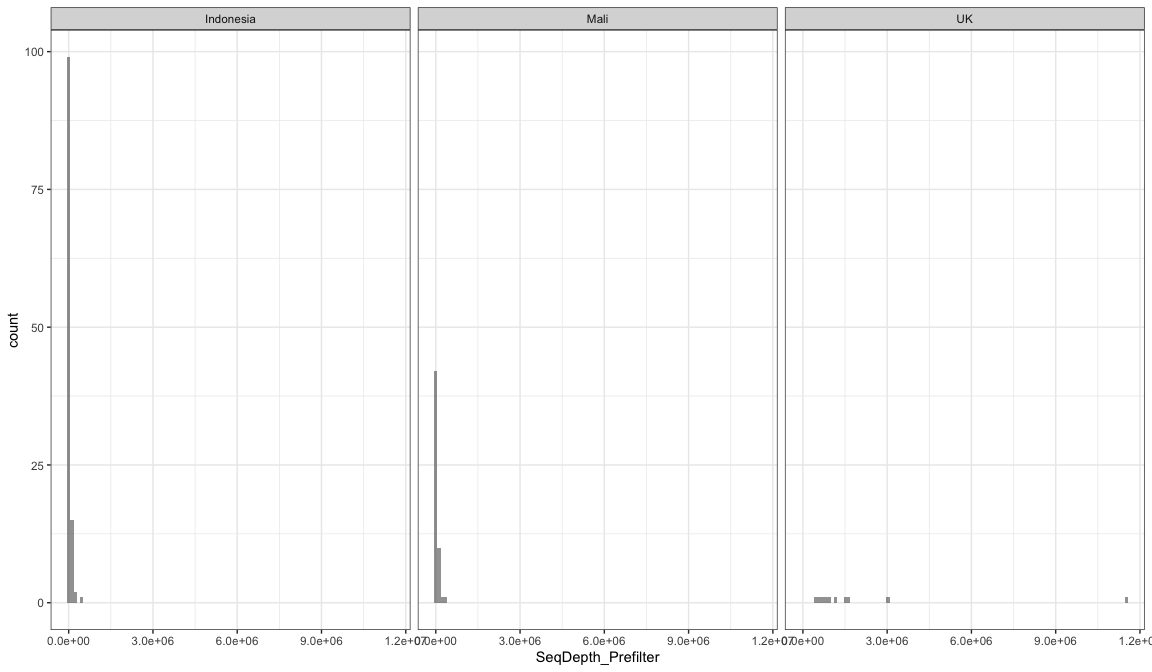
\includegraphics{1.IndonesianVsMaliAndTBControls_CLRMethod_files/figure-latex/unnamed-chunk-7-1.pdf}
With a higher sequencing depth, you can afford to play around with
thresholding, however for the Indonesian dataset, the sequencing depth
is variable and quite low in some samples. Therefore, pushing this
threshold up too high will eliminate rare taxa, especially given that we
didn't have a high library size to begin with.

Although our starting library size is small, let's explore the data a
bit by looking at the effect of removing singletons.

A great tool to do this is raraefaction curves. Rarefaction curves are
commonly used in microbiomics to estimate 1) species richness and 2)
determine how extensively a library was sampled. For the first point,
it's nearly impossible to capture all species within a community, and
therefore this allows for a way to estimate the total species we would
expect to find by extrapolating the curve within the rarefaction plot. A
rarefaction curve will (if sampled to a high enough depth) asymptote,
and this point is regarded as the estimate of the total number of
species within that community.

For the second point, we can also use the asymptote of the curve to see
how extensively we sampled. If the curve has not started to flatten off,
we have not captured everything.

Lets see how rarefaction looks like when we remove singletons and when
we remove 5 counts.

\begin{Shaded}
\begin{Highlighting}[]
\CommentTok{# Separate species' abundances and taxonomy columns}
\NormalTok{rarecurve_counts <-}\StringTok{ }\KeywordTok{otu_table}\NormalTok{(merged_phylo_counts)}
\NormalTok{col <-}\StringTok{ }\KeywordTok{c}\NormalTok{(}\KeywordTok{rep}\NormalTok{(IndonesiaCol,}\KeywordTok{sum}\NormalTok{(}\KeywordTok{sample_data}\NormalTok{(merged_phylo_counts)[,}\StringTok{"SamplePop"}\NormalTok{]}\OperatorTok{==}\StringTok{"Indonesia"}\NormalTok{)),}\KeywordTok{rep}\NormalTok{(MaliCol,}\KeywordTok{sum}\NormalTok{(}\KeywordTok{sample_data}\NormalTok{(merged_phylo_counts)[,}\StringTok{"SamplePop"}\NormalTok{]}\OperatorTok{==}\StringTok{"Mali"}\NormalTok{)),}\KeywordTok{rep}\NormalTok{(UKCol,}\KeywordTok{sum}\NormalTok{(}\KeywordTok{sample_data}\NormalTok{(merged_phylo_counts)[,}\StringTok{"SamplePop"}\NormalTok{]}\OperatorTok{==}\StringTok{"UK"}\NormalTok{)))}
\CommentTok{# Try with different filtering thresholds:}
\ControlFlowTok{for}\NormalTok{ (i }\ControlFlowTok{in} \KeywordTok{c}\NormalTok{(}\DecValTok{1}\NormalTok{,}\DecValTok{5}\NormalTok{))\{}
\NormalTok{    rarecurve_counts[rarecurve_counts}\OperatorTok{<=}\NormalTok{i]<-}\DecValTok{0}
    \KeywordTok{rarecurve}\NormalTok{(}\KeywordTok{t}\NormalTok{(}\KeywordTok{otu_table}\NormalTok{(rarecurve_counts, }\DataTypeTok{taxa_are_rows =} \OtherTok{TRUE}\NormalTok{)), }\DataTypeTok{step=}\DecValTok{200}\NormalTok{, }\DataTypeTok{col=}\NormalTok{col,}\DataTypeTok{label=}\NormalTok{F, }\DataTypeTok{xlab=}\StringTok{"Counts"}\NormalTok{,}\DataTypeTok{ylab=}\StringTok{"Number Species"}\NormalTok{,}\DataTypeTok{main=}\KeywordTok{paste}\NormalTok{(}\StringTok{"Removing Reads"}\NormalTok{,i,}\StringTok{"And Below"}\NormalTok{,}\DataTypeTok{sep=}\StringTok{" "}\NormalTok{),}\DataTypeTok{xlim=}\KeywordTok{c}\NormalTok{(}\DecValTok{0}\NormalTok{,}\DecValTok{50000}\NormalTok{))}
\NormalTok{\}}

\NormalTok{Indonesian_subset <-}\StringTok{ }\KeywordTok{prune_taxa}\NormalTok{(}\KeywordTok{taxa_sums}\NormalTok{(Indonesian_subset) }\OperatorTok{>}\StringTok{ }\DecValTok{0}\NormalTok{, Indonesian_subset)}
\NormalTok{rarecurve_counts <-}\StringTok{ }\KeywordTok{otu_table}\NormalTok{(Indonesian_subset)}
\NormalTok{col <-}\StringTok{ }\NormalTok{IndonesiaCol}
\ControlFlowTok{for}\NormalTok{ (i }\ControlFlowTok{in} \KeywordTok{c}\NormalTok{(}\DecValTok{1}\NormalTok{,}\DecValTok{5}\NormalTok{))\{}
\NormalTok{    rarecurve_counts[rarecurve_counts}\OperatorTok{<=}\NormalTok{i]<-}\DecValTok{0}
    \KeywordTok{rarecurve}\NormalTok{(}\KeywordTok{t}\NormalTok{(}\KeywordTok{otu_table}\NormalTok{(rarecurve_counts, }\DataTypeTok{taxa_are_rows =} \OtherTok{TRUE}\NormalTok{)), }\DataTypeTok{step=}\DecValTok{200}\NormalTok{, }\DataTypeTok{col=}\NormalTok{col,}\DataTypeTok{label=}\NormalTok{F, }\DataTypeTok{xlab=}\StringTok{"Counts"}\NormalTok{,}\DataTypeTok{ylab=}\StringTok{"Number Species"}\NormalTok{,}\DataTypeTok{main=}\KeywordTok{paste}\NormalTok{(}\StringTok{"Removing Reads"}\NormalTok{,i,}\StringTok{"And Below }\CharTok{\textbackslash{}n}\StringTok{Indonesian Samples"}\NormalTok{,}\DataTypeTok{sep=}\StringTok{" "}\NormalTok{),}\DataTypeTok{xlim=}\KeywordTok{c}\NormalTok{(}\DecValTok{0}\NormalTok{,}\DecValTok{10000}\NormalTok{))}
\NormalTok{\}}
\end{Highlighting}
\end{Shaded}

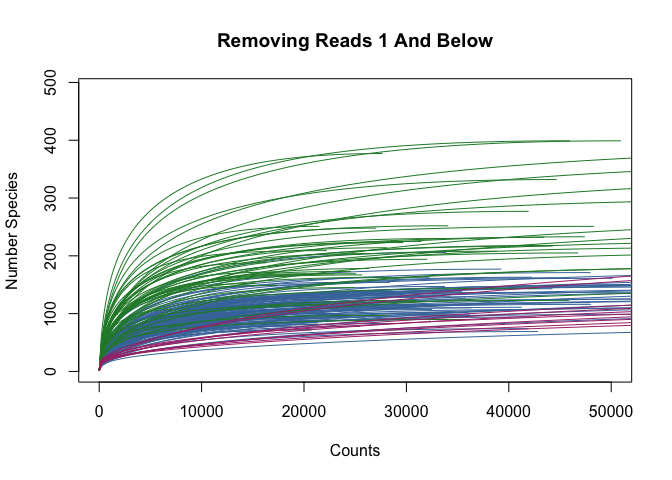
\includegraphics[width=0.5\linewidth]{1.IndonesianVsMaliAndTBControls_CLRMethod_files/figure-latex/unnamed-chunk-8-1}
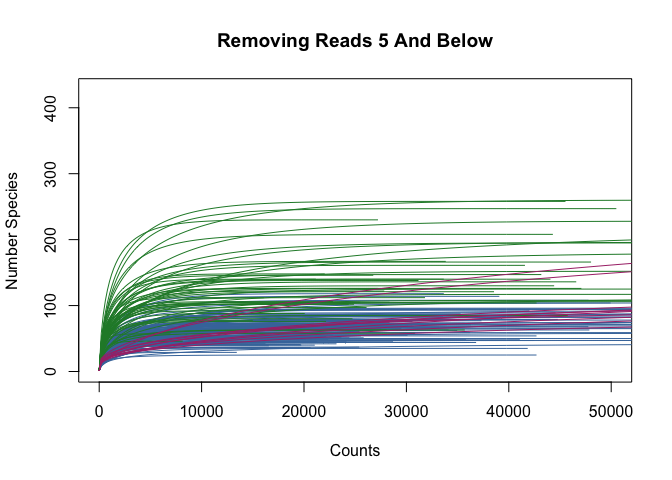
\includegraphics[width=0.5\linewidth]{1.IndonesianVsMaliAndTBControls_CLRMethod_files/figure-latex/unnamed-chunk-8-2}
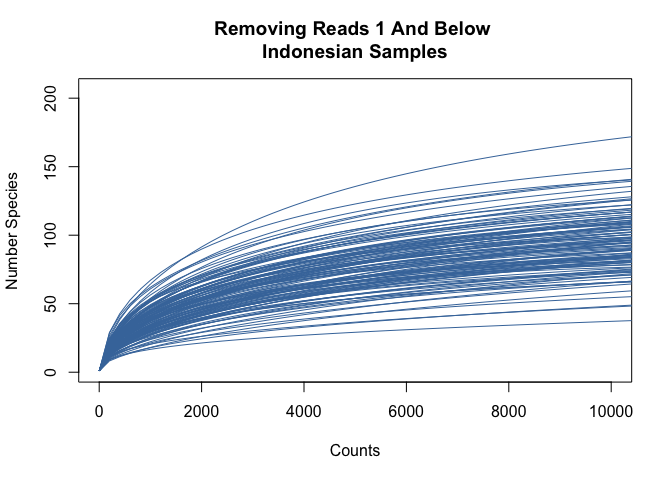
\includegraphics[width=0.5\linewidth]{1.IndonesianVsMaliAndTBControls_CLRMethod_files/figure-latex/unnamed-chunk-8-3}
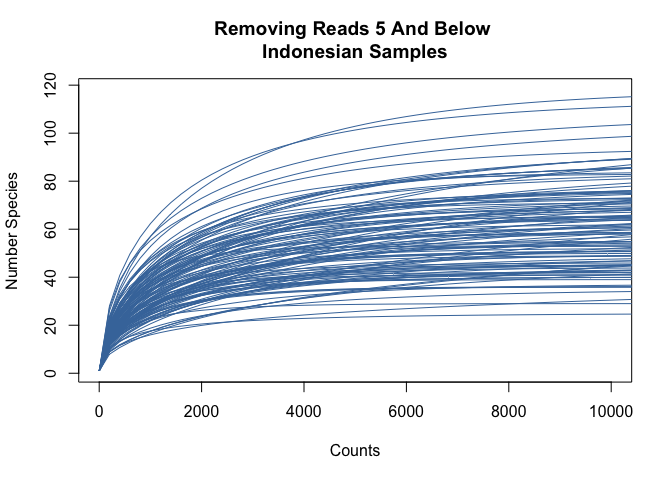
\includegraphics[width=0.5\linewidth]{1.IndonesianVsMaliAndTBControls_CLRMethod_files/figure-latex/unnamed-chunk-8-4}

From the rarefaction curves, we can notice a few things. For one, the
library size needed to capture all of the taxa is quite variable between
studies and individuals. For example, some samples in the Indonesian
study are not very diverse and don't need that many reads to capture all
of the taxa (\textless{}5,000). In contrast to this, the Malian study
(in green) is the most diverse, with over 20,000 reads necessary to
capture the full diversity in some samples.

We might also notice that when removing we remove reads 5 and below
(shown on the right hand side), the curve asymptotes much sooner. This
is because you need more reads to detect rare species, and therefore
removing reads 5 and below eliminates some of these rare species.

As mentioned before, because our starting read depth is small, we will
stick with removing singletons. We will also make a copy of the
unfiltered data for downstream use.

\begin{Shaded}
\begin{Highlighting}[]
\CommentTok{# Filter out singletons}
\KeywordTok{otu_table}\NormalTok{(merged_phylo_counts)[}\KeywordTok{otu_table}\NormalTok{(merged_phylo_counts)}\OperatorTok{<=}\DecValTok{1}\NormalTok{]<-}\DecValTok{0}
\NormalTok{merged_phylo_counts <-}\StringTok{ }\KeywordTok{prune_taxa}\NormalTok{(}\KeywordTok{taxa_sums}\NormalTok{(merged_phylo_counts) }\OperatorTok{>}\StringTok{ }\DecValTok{0}\NormalTok{, merged_phylo_counts)}
\CommentTok{# add sequencing depth information after filtering out singletons}
\NormalTok{SeqDepth_noSingletons =}\StringTok{ }\KeywordTok{colSums}\NormalTok{(}\KeywordTok{otu_table}\NormalTok{(merged_phylo_counts))}
\KeywordTok{sample_data}\NormalTok{(merged_phylo_counts)}\OperatorTok{$}\NormalTok{SeqDepth_noSingletons =}\StringTok{ }\NormalTok{SeqDepth_noSingletons}
\end{Highlighting}
\end{Shaded}

\hypertarget{removing-humans-and-plants}{%
\subsection{Removing humans and
plants}\label{removing-humans-and-plants}}

From the script X, we saw that human reads and viridiplantae are not of
interest because of X. We'll filter these out.

\begin{Shaded}
\begin{Highlighting}[]
\CommentTok{# Filter out Viridiplantae }
\NormalTok{merged_phylo_counts <-}\StringTok{ }\KeywordTok{subset_taxa}\NormalTok{(merged_phylo_counts, (Kingdom}\OperatorTok{!=}\StringTok{"Viridiplantae"}\NormalTok{))}
\NormalTok{merged_phylo_counts <-}\StringTok{ }\KeywordTok{prune_taxa}\NormalTok{(}\KeywordTok{taxa_sums}\NormalTok{(merged_phylo_counts) }\OperatorTok{>}\StringTok{ }\DecValTok{0}\NormalTok{, merged_phylo_counts)}
\CommentTok{# add sequencing depth information after filtering out plants}
\NormalTok{SeqDepth_noViridiplantae =}\StringTok{ }\KeywordTok{colSums}\NormalTok{(}\KeywordTok{otu_table}\NormalTok{(merged_phylo_counts))}
\KeywordTok{sample_data}\NormalTok{(merged_phylo_counts)}\OperatorTok{$}\NormalTok{SeqDepth_noViridiplantae =}\StringTok{ }\NormalTok{SeqDepth_noViridiplantae}

\CommentTok{# Filter out Chordata}
\NormalTok{merged_phylo_counts <-}\StringTok{ }\KeywordTok{subset_taxa}\NormalTok{(merged_phylo_counts, (Phylum}\OperatorTok{!=}\StringTok{"Chordata"}\NormalTok{))}
\NormalTok{merged_phylo_counts <-}\StringTok{ }\KeywordTok{prune_taxa}\NormalTok{(}\KeywordTok{taxa_sums}\NormalTok{(merged_phylo_counts) }\OperatorTok{>}\StringTok{ }\DecValTok{0}\NormalTok{, merged_phylo_counts)}
\CommentTok{# add sequencing depth information after filtering out Metazoa}
\NormalTok{SeqDepth_noChordata =}\StringTok{ }\KeywordTok{colSums}\NormalTok{(}\KeywordTok{otu_table}\NormalTok{(merged_phylo_counts))}
\KeywordTok{sample_data}\NormalTok{(merged_phylo_counts)}\OperatorTok{$}\NormalTok{SeqDepth_noChordata =}\StringTok{ }\NormalTok{SeqDepth_noChordata}

\CommentTok{# Filter out Metazoa}
\NormalTok{merged_phylo_counts <-}\StringTok{ }\KeywordTok{subset_taxa}\NormalTok{(merged_phylo_counts, (Kingdom}\OperatorTok{!=}\StringTok{"Metazoa"}\NormalTok{))}
\NormalTok{merged_phylo_counts <-}\StringTok{ }\KeywordTok{prune_taxa}\NormalTok{(}\KeywordTok{taxa_sums}\NormalTok{(merged_phylo_counts) }\OperatorTok{>}\StringTok{ }\DecValTok{0}\NormalTok{, merged_phylo_counts)}
\CommentTok{# add sequencing depth information after filtering out Metazoa}
\NormalTok{SeqDepth_noMetazoa =}\StringTok{ }\KeywordTok{colSums}\NormalTok{(}\KeywordTok{otu_table}\NormalTok{(merged_phylo_counts))}
\KeywordTok{sample_data}\NormalTok{(merged_phylo_counts)}\OperatorTok{$}\NormalTok{SeqDepth_noMetazoa =}\StringTok{ }\NormalTok{SeqDepth_noMetazoa}
\end{Highlighting}
\end{Shaded}

Now that we've done all of the filtering, we can plot the final library
sizes.

\begin{Shaded}
\begin{Highlighting}[]
\CommentTok{# barplot of library sizes}
\KeywordTok{ggplot}\NormalTok{(}\KeywordTok{meta}\NormalTok{(merged_phylo_counts), }\KeywordTok{aes}\NormalTok{(SampleName, SeqDepth_noMetazoa)) }\OperatorTok{+}\StringTok{ }\KeywordTok{geom_bar}\NormalTok{(}\DataTypeTok{stat =} \StringTok{"identity"}\NormalTok{, }\KeywordTok{aes}\NormalTok{(}\DataTypeTok{fill =}\NormalTok{ SamplePop)) }\OperatorTok{+}
\KeywordTok{scale_fill_manual}\NormalTok{(}\DataTypeTok{values =} \KeywordTok{c}\NormalTok{(IndonesiaCol,MaliCol,UKCol)) }\OperatorTok{+}\StringTok{ }\KeywordTok{rotate_x_text}\NormalTok{()}
\end{Highlighting}
\end{Shaded}

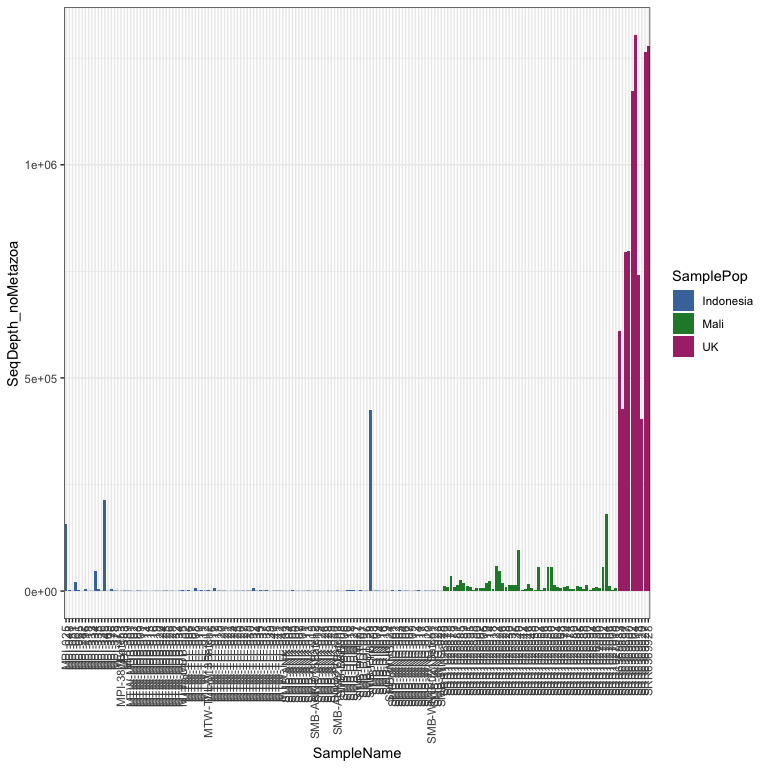
\includegraphics{1.IndonesianVsMaliAndTBControls_CLRMethod_files/figure-latex/unnamed-chunk-11-1.pdf}
We can see that the library sizes are highly uneven, with the Indonesian
data having the lowest sampling depth (with the exception of a few
samples) and the UK dataset hacing the highest library depth.

\hypertarget{summarising-the-data}{%
\subsection{Summarising the data}\label{summarising-the-data}}

The final step us is to summarise the data and see how many reads we
lost at each filtering step.

\begin{Shaded}
\begin{Highlighting}[]
\NormalTok{FilteringSummary =}\StringTok{ }\KeywordTok{sample_data}\NormalTok{(merged_phylo_counts)[,}\KeywordTok{c}\NormalTok{(}\StringTok{"SamplePop"}\NormalTok{,}\StringTok{"SeqDepth_Prefilter"}\NormalTok{,}\StringTok{"SeqDepth_noSingletons"}\NormalTok{,}\StringTok{"SeqDepth_noViridiplantae"}\NormalTok{,}\StringTok{"SeqDepth_noChordata"}\NormalTok{,}\StringTok{"SeqDepth_noMetazoa"}\NormalTok{)]}

\CommentTok{# melt df and plot}
\NormalTok{melted_FilteringSummary =}\StringTok{ }\KeywordTok{melt}\NormalTok{(FilteringSummary)}
\KeywordTok{ggplot}\NormalTok{(melted_FilteringSummary, }\KeywordTok{aes}\NormalTok{(}\DataTypeTok{x=}\NormalTok{variable, }\DataTypeTok{y=}\NormalTok{value, }\DataTypeTok{fill=}\NormalTok{SamplePop)) }\OperatorTok{+}
\StringTok{  }\KeywordTok{geom_violin}\NormalTok{(}\DataTypeTok{alpha=}\FloatTok{0.8}\NormalTok{) }\OperatorTok{+}\StringTok{ }\KeywordTok{theme_bw}\NormalTok{() }\OperatorTok{+}\StringTok{ }\KeywordTok{ylab}\NormalTok{(}\StringTok{"Spearman pairwise correlation"}\NormalTok{) }\OperatorTok{+}
\StringTok{  }\KeywordTok{theme}\NormalTok{(}\DataTypeTok{axis.title.x=}\KeywordTok{element_blank}\NormalTok{(), }\DataTypeTok{axis.text.x =} \KeywordTok{element_text}\NormalTok{(}\DataTypeTok{angle =} \DecValTok{90}\NormalTok{)) }\OperatorTok{+}\StringTok{ }\KeywordTok{scale_fill_manual}\NormalTok{(}\DataTypeTok{values =} \KeywordTok{c}\NormalTok{(IndonesiaCol,MaliCol,UKCol)) }\OperatorTok{+}
\StringTok{  }\KeywordTok{geom_boxplot}\NormalTok{(}\DataTypeTok{color=}\StringTok{"black"}\NormalTok{,}\DataTypeTok{width=}\FloatTok{0.2}\NormalTok{, }\DataTypeTok{alpha =} \FloatTok{0.7}\NormalTok{) }\OperatorTok{+}\StringTok{ }\KeywordTok{facet_wrap}\NormalTok{(}\OperatorTok{~}\StringTok{ }\NormalTok{SamplePop, }\DataTypeTok{scales =} \StringTok{"free"}\NormalTok{)}
\end{Highlighting}
\end{Shaded}

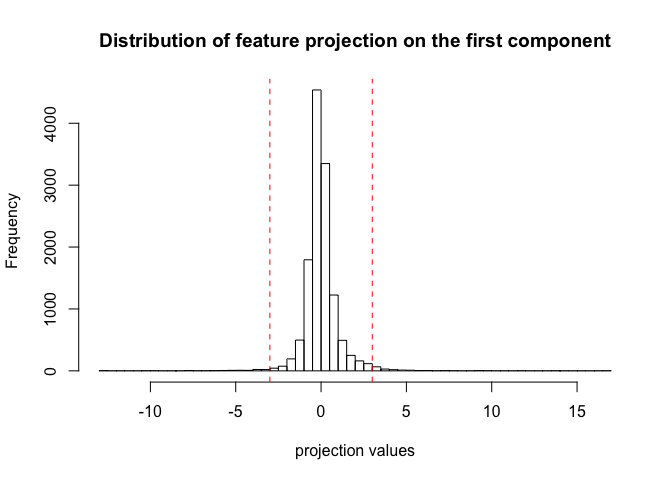
\includegraphics{1.IndonesianVsMaliAndTBControls_CLRMethod_files/figure-latex/unnamed-chunk-12-1.pdf}

We can see that in the Indonesian and Malian dataset, most of the reads
are removed when removing Chordates, however for the UK dataset, most
reads are removed when removing Metazoa. For the UK datset, this is due
to a high number of reads mapping to molluscs, as seen in script X.

\hypertarget{data-normalisation}{%
\section{Data normalisation}\label{data-normalisation}}

The library sizes between samples and groups is highly variable, and
therefore comparing the data to each other will result in biased
results.

There are two ways of handling this: 1. Performing a transformation of
the data 2. Rarefying the data

\hypertarget{centered-log-ration-transformation}{%
\subsection{Centered log-ration
transformation}\label{centered-log-ration-transformation}}

Taxa can be viewed by their relative abundance, however changes in the
abundance of one taxon will result in changing the abundance of other
taxa.

One of the ways to handle this is to transform the data using Centered
Log Ratio (CLR)transformation. CLR data shows how OTUs behave relative
to the per-sample average and is a commonly-used data transformation
method in microbiomics.

Another cool thing about using CLR-transformed data is that it is not
affected by sequencing depth. This excerpt from a paper by
\href{https://www.ncbi.nlm.nih.gov/pmc/articles/PMC5695134/}{Gloor et
al} explains this really well:

``The clr-transformed values are scale-invariant; that is the same ratio
is expected to be obtained in a sample with few read counts or an
identical sample with many read counts, only the precision of the clr
estimate is affected. This is elaborated in the ``Probability'' and
``Log-ratio transformations'' section in the Supplement, but the
consequence is that count normalization is unnecessary and indeed,
undesirable since information on precision is lost."

Unfortunately, one of the disadvantages to using CLR-transformed data is
that it can't be used in diversity estimates, and it's also hard to
visualise.

Becasue CLR data is an informative measure of our data, I'll first
explore sample grouping using this method.

The first step to performing a CLR transformation on the data is to add
an offset of 1 to the counts. This is necessary, since performing a log
on 0 values is undefined. We'll then perform a log ratio transformation
of the data using the mixOmics package.

\begin{Shaded}
\begin{Highlighting}[]
\NormalTok{offset_otu=}\KeywordTok{otu_table}\NormalTok{(merged_phylo_counts)}\OperatorTok{+}\DecValTok{1}
\NormalTok{transform_counts=}\KeywordTok{t}\NormalTok{(}\KeywordTok{otu_table}\NormalTok{(offset_otu))}
\NormalTok{data_clr <-}\StringTok{ }\KeywordTok{logratio.transfo}\NormalTok{(}\KeywordTok{as.matrix}\NormalTok{(transform_counts), }\DataTypeTok{logratio =} \StringTok{'CLR'}\NormalTok{, }\DataTypeTok{offset =} \DecValTok{0}\NormalTok{) }
\end{Highlighting}
\end{Shaded}

\hypertarget{sample-grouping}{%
\subsubsection{Sample grouping}\label{sample-grouping}}

Now that we've transformed our data, we can make a PCA plot to see how
each sample clusters. The current obect we have is a CLR-class object.
You can plot this type of data object easily with miOmics, however I
prefer the visualisation that phyloseq offers (you can't alter the PCA
plots that much in mixOmics). So, we'll turn the clr object back into a
phyloseq object and make an ordination plot of the data.

!Note: When Euclidean distances are used in PCoA plots, it is
\href{http://ordination.okstate.edu/overview.htm}{equivalent to a PCA
plot}.

\begin{Shaded}
\begin{Highlighting}[]
\CommentTok{# Make a duplicated phyloseq object to use for plotting}
\KeywordTok{class}\NormalTok{(data_clr)=}\StringTok{"matrix"}
\end{Highlighting}
\end{Shaded}

\begin{verbatim}
## Warning in class(data_clr) = "matrix": Setting class(x) to "matrix" sets
## attribute to NULL; result will no longer be an S4 object
\end{verbatim}

\begin{Shaded}
\begin{Highlighting}[]
\NormalTok{taxa =}\StringTok{ }\KeywordTok{otu_table}\NormalTok{(}\KeywordTok{t}\NormalTok{(data_clr), }\DataTypeTok{taxa_are_rows =} \OtherTok{TRUE}\NormalTok{)}
\NormalTok{merged_phylo_counts_clr=merged_phylo_counts}
\KeywordTok{otu_table}\NormalTok{(merged_phylo_counts_clr)=taxa}

\NormalTok{out.wuf.log <-}\StringTok{ }\KeywordTok{ordinate}\NormalTok{(merged_phylo_counts_clr, }\DataTypeTok{method =} \StringTok{"PCoA"}\NormalTok{, }\DataTypeTok{distance =} \StringTok{"euclidean"}\NormalTok{)}
\KeywordTok{plot_ordination}\NormalTok{(merged_phylo_counts_clr, out.wuf.log, }\DataTypeTok{color=}\StringTok{"SamplePop"}\NormalTok{, }\DataTypeTok{axes =} \DecValTok{1}\OperatorTok{:}\DecValTok{2}\NormalTok{, }\DataTypeTok{label=}\StringTok{"SampleName"}\NormalTok{) }\OperatorTok{+}\StringTok{ }\KeywordTok{scale_colour_manual}\NormalTok{(}\DataTypeTok{values=}\KeywordTok{c}\NormalTok{(IndonesiaCol,MaliCol,UKCol))}
\end{Highlighting}
\end{Shaded}

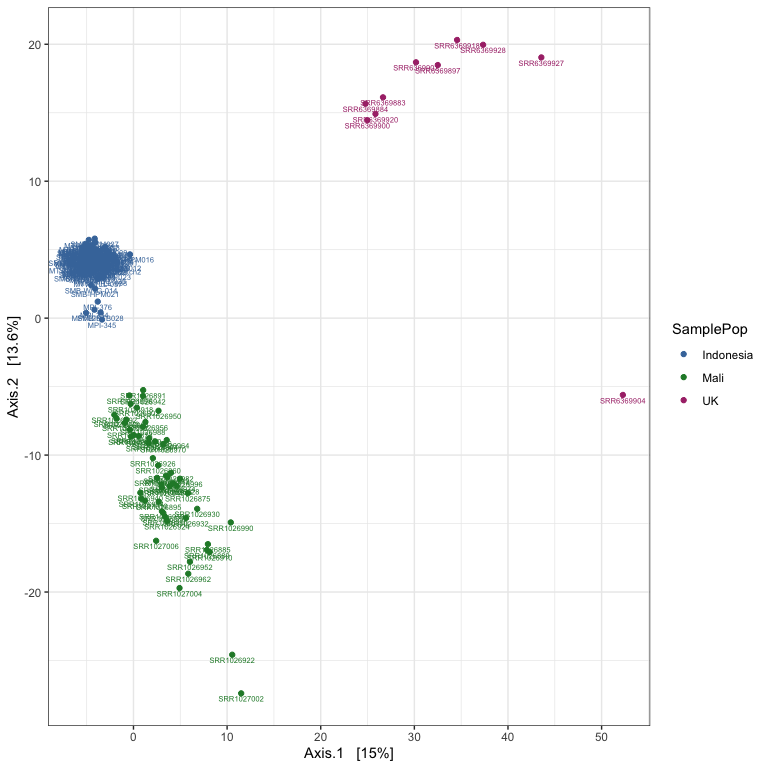
\includegraphics{1.IndonesianVsMaliAndTBControls_CLRMethod_files/figure-latex/unnamed-chunk-14-1.pdf}
We can see that the first principal component is separating the three
studies apart. This is also supported by hierarchical clustering of the
clr-tranformed data by euclidean distance.

\begin{Shaded}
\begin{Highlighting}[]
\NormalTok{ps_otu <-}\StringTok{ }\KeywordTok{data.frame}\NormalTok{(phyloseq}\OperatorTok{::}\KeywordTok{otu_table}\NormalTok{(merged_phylo_counts_clr))}
\NormalTok{ps_otu <-}\StringTok{ }\KeywordTok{t}\NormalTok{(ps_otu)}
\NormalTok{bc_dist <-}\StringTok{ }\NormalTok{vegan}\OperatorTok{::}\KeywordTok{vegdist}\NormalTok{(ps_otu, }\DataTypeTok{method =} \StringTok{"euclidean"}\NormalTok{)}
\NormalTok{ward <-}\StringTok{ }\KeywordTok{as.dendrogram}\NormalTok{(}\KeywordTok{hclust}\NormalTok{(bc_dist, }\DataTypeTok{method =} \StringTok{"ward.D2"}\NormalTok{))}
\CommentTok{#Provide color codes}
\NormalTok{meta <-}\StringTok{ }\KeywordTok{data.frame}\NormalTok{(phyloseq}\OperatorTok{::}\KeywordTok{sample_data}\NormalTok{(merged_phylo_counts_clr))}
\NormalTok{colorCode <-}\StringTok{ }\KeywordTok{c}\NormalTok{(}\DataTypeTok{Indonesia =}\NormalTok{ IndonesiaCol, }\StringTok{`}\DataTypeTok{Mali}\StringTok{`}\NormalTok{ =}\StringTok{ }\NormalTok{MaliCol, }\StringTok{`}\DataTypeTok{UK}\StringTok{`}\NormalTok{ =}\StringTok{ }\NormalTok{UKCol)}
\KeywordTok{labels_colors}\NormalTok{(ward) <-}\StringTok{ }\NormalTok{colorCode[meta}\OperatorTok{$}\NormalTok{SamplePop][}\KeywordTok{order.dendrogram}\NormalTok{(ward)]}
\CommentTok{#Plot}
\KeywordTok{plot}\NormalTok{(ward)}
\end{Highlighting}
\end{Shaded}

\begin{center}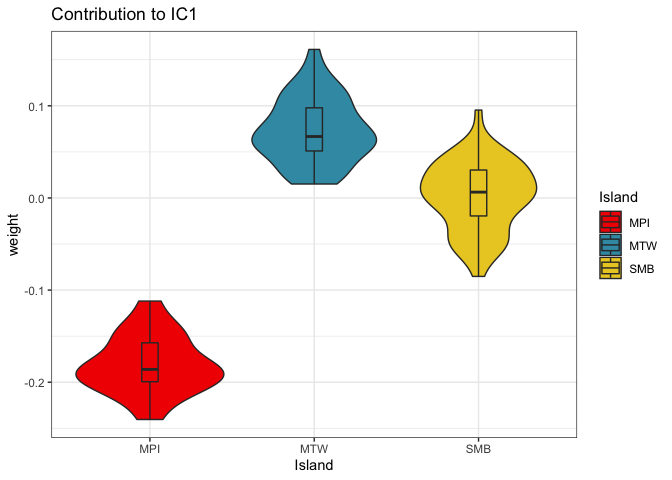
\includegraphics{1.IndonesianVsMaliAndTBControls_CLRMethod_files/figure-latex/unnamed-chunk-15-1} \end{center}

If we look at the second principal component, we can see that it splits
the UK samples apart from the Malian and Indonesian samples, while the
Indonesian and Malian samples come together. Finally, axis three
separates the three studies from an outlier sample in the UK study -
SRR6369904. We'll investigate why this samples is an outlier (a bit
later).

\begin{Shaded}
\begin{Highlighting}[]
\KeywordTok{plot_ordination}\NormalTok{(merged_phylo_counts_clr, out.wuf.log, }\DataTypeTok{color=}\StringTok{"SamplePop"}\NormalTok{, }\DataTypeTok{axes =} \DecValTok{2}\OperatorTok{:}\DecValTok{3}\NormalTok{, }\DataTypeTok{label=}\StringTok{"SampleName"}\NormalTok{) }\OperatorTok{+}\StringTok{ }\KeywordTok{scale_colour_manual}\NormalTok{(}\DataTypeTok{values=}\KeywordTok{c}\NormalTok{(IndonesiaCol,MaliCol,UKCol))}
\end{Highlighting}
\end{Shaded}

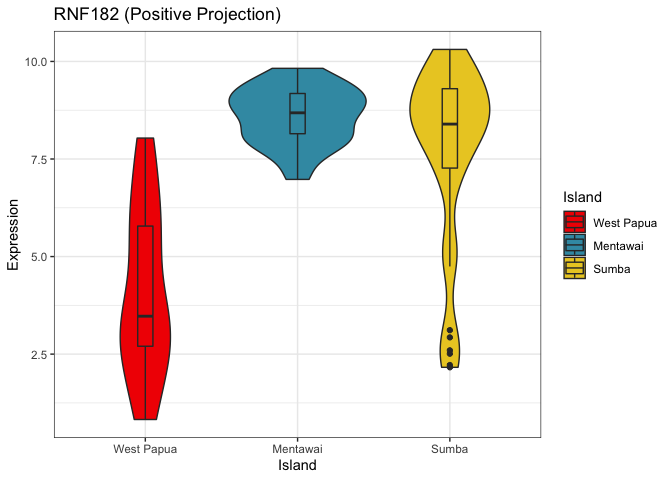
\includegraphics{1.IndonesianVsMaliAndTBControls_CLRMethod_files/figure-latex/unnamed-chunk-16-1.pdf}

\begin{Shaded}
\begin{Highlighting}[]
\KeywordTok{plot_ordination}\NormalTok{(merged_phylo_counts_clr, out.wuf.log, }\DataTypeTok{color=}\StringTok{"SamplePop"}\NormalTok{, }\DataTypeTok{axes =} \DecValTok{3}\OperatorTok{:}\DecValTok{4}\NormalTok{, }\DataTypeTok{label=}\StringTok{"SampleName"}\NormalTok{) }\OperatorTok{+}\StringTok{ }\KeywordTok{scale_colour_manual}\NormalTok{(}\DataTypeTok{values=}\KeywordTok{c}\NormalTok{(IndonesiaCol,MaliCol,UKCol))}
\end{Highlighting}
\end{Shaded}

\includegraphics{1.IndonesianVsMaliAndTBControls_CLRMethod_files/figure-latex/unnamed-chunk-16-2.pdf}

\hypertarget{relative-frequency-of-taxa}{%
\section{Relative frequency of taxa}\label{relative-frequency-of-taxa}}

One of the questions we're most interested in when investigating these
samples is: what is in the data? One of the ways to do this is by
visualising the data itself. A common way to do this is by looking at a
stacked barplot, one for each sample, composed of the relative frequency
of taxa in that sample.

Why do we look at relative frequency? As we've seen before, our library
sizes are uneven, and therefore we want to see what the proportion of
each taxa is in each sample. However, compositional data does not
account for the fact that as one species goes up, it will force another
species to go down (i.e., it is bounded).

I'll try to solve this proble in a few ways. The first way is by
plotting the relative taxa, then seeing how this compares to the
rarefied data. Finally, I'll plot the CLR data (which is unconstrained)
to see how this looks.

To visualise relative frequency, I want to show my taxa at the family
level, however since there are over 450 unique taxa at the family level,
this would be difficult to visualise with so many colours. Instead,
we'll make a new taxa variable which combines Superkingdom information
with Family-level information. This way, we can highlight colours by
superkingdom (which isn't so visually overwhelming), and still preserve
Family-level information.

\hypertarget{unsubsampled-compositional-data}{%
\subsection{Unsubsampled compositional
data}\label{unsubsampled-compositional-data}}

\begin{Shaded}
\begin{Highlighting}[]
\CommentTok{# add a new column containing family names and superkingdom}
\KeywordTok{tax_table}\NormalTok{(merged_phylo_counts)[,}\StringTok{"Superkingdom"}\NormalTok{] =}\StringTok{ }\KeywordTok{paste}\NormalTok{(}\KeywordTok{tax_table}\NormalTok{(merged_phylo_counts)[,}\StringTok{"Superkingdom"}\NormalTok{], }\KeywordTok{tax_table}\NormalTok{(merged_phylo_counts)[,}\StringTok{"Family"}\NormalTok{], }\DataTypeTok{sep=}\StringTok{"_"}\NormalTok{)}
\KeywordTok{tax_table}\NormalTok{(merged_phylo_counts)[,}\StringTok{"Superkingdom"}\NormalTok{] <-}\StringTok{ }\KeywordTok{gsub}\NormalTok{(}\StringTok{"Bacteria_$"}\NormalTok{, }\StringTok{"Bacteria_unclassified"}\NormalTok{, }\KeywordTok{tax_table}\NormalTok{(merged_phylo_counts)[,}\StringTok{"Superkingdom"}\NormalTok{])}
\KeywordTok{tax_table}\NormalTok{(merged_phylo_counts)[,}\StringTok{"Superkingdom"}\NormalTok{] <-}\StringTok{ }\KeywordTok{gsub}\NormalTok{(}\StringTok{"Eukaryota_$"}\NormalTok{, }\StringTok{"Eukaryota_unclassified"}\NormalTok{, }\KeywordTok{tax_table}\NormalTok{(merged_phylo_counts)[,}\StringTok{"Superkingdom"}\NormalTok{])}
\KeywordTok{tax_table}\NormalTok{(merged_phylo_counts)[,}\StringTok{"Superkingdom"}\NormalTok{] <-}\StringTok{ }\KeywordTok{gsub}\NormalTok{(}\StringTok{"Viruses_$"}\NormalTok{, }\StringTok{"Viruses_unclassified"}\NormalTok{, }\KeywordTok{tax_table}\NormalTok{(merged_phylo_counts)[,}\StringTok{"Superkingdom"}\NormalTok{])}
\end{Highlighting}
\end{Shaded}

As pointed out, we have a lot of taxa at the family level, and it would
be hard to look over everything at once. Instead, we can focus on the
most prevalent taxa and highlight everything else in another colour.

Here, I chose to highlight the top 20 taxa, since that's still
representative while not being too visually exhausting.

\begin{Shaded}
\begin{Highlighting}[]
\NormalTok{aggregated_phyloCounts <-}\StringTok{ }\KeywordTok{aggregate_top_taxa}\NormalTok{(merged_phylo_counts, }\StringTok{"Superkingdom"}\NormalTok{, }\DataTypeTok{top =} \DecValTok{20}\NormalTok{)}
\CommentTok{# transform to relative counts}
\NormalTok{relative_phyloCounts <-}\StringTok{ }\NormalTok{microbiome}\OperatorTok{::}\KeywordTok{transform}\NormalTok{(aggregated_phyloCounts, }\StringTok{"compositional"}\NormalTok{)}
\CommentTok{# Remove weird extra family names added at the end of Superkingdom names}
\KeywordTok{tax_table}\NormalTok{(relative_phyloCounts)[,}\StringTok{"Superkingdom"}\NormalTok{] <-}\StringTok{ }\KeywordTok{paste}\NormalTok{(}\KeywordTok{sapply}\NormalTok{(}\KeywordTok{strsplit}\NormalTok{(}\KeywordTok{taxa_names}\NormalTok{(relative_phyloCounts), }\StringTok{"[_.]"}\NormalTok{), }\StringTok{`}\DataTypeTok{[}\StringTok{`}\NormalTok{, }\DecValTok{1}\NormalTok{), }\KeywordTok{sapply}\NormalTok{(}\KeywordTok{strsplit}\NormalTok{(}\KeywordTok{taxa_names}\NormalTok{(relative_phyloCounts), }\StringTok{"[_.]"}\NormalTok{), }\StringTok{`}\DataTypeTok{[}\StringTok{`}\NormalTok{, }\DecValTok{2}\NormalTok{), }\DataTypeTok{sep=}\StringTok{"_"}\NormalTok{)}
\CommentTok{# Change "Other_NA" to just "Other"}
\KeywordTok{tax_table}\NormalTok{(relative_phyloCounts)[,}\StringTok{"Superkingdom"}\NormalTok{][}\KeywordTok{grep}\NormalTok{(}\StringTok{"Other"}\NormalTok{, }\KeywordTok{taxa_names}\NormalTok{(relative_phyloCounts))] =}\StringTok{ "Other"}

\CommentTok{# Plot}
\NormalTok{p=}\KeywordTok{plot_bar}\NormalTok{(relative_phyloCounts, }\DataTypeTok{fill =} \StringTok{"Superkingdom"}\NormalTok{)}

\CommentTok{# set colour palette}
\NormalTok{families=}\KeywordTok{levels}\NormalTok{(p}\OperatorTok{$}\NormalTok{data}\OperatorTok{$}\NormalTok{Superkingdom)}
\CommentTok{# get number of families in each kingdom}
\KeywordTok{table}\NormalTok{(}\KeywordTok{sapply}\NormalTok{(}\KeywordTok{strsplit}\NormalTok{(families, }\StringTok{"[_.]"}\NormalTok{), }\StringTok{`}\DataTypeTok{[}\StringTok{`}\NormalTok{, }\DecValTok{1}\NormalTok{))}
\end{Highlighting}
\end{Shaded}

\begin{verbatim}
## 
##   Archaea  Bacteria Eukaryota     Other   Viruses 
##         1        15         2         1         2
\end{verbatim}

\begin{Shaded}
\begin{Highlighting}[]
\NormalTok{PaletteArchaea =}\StringTok{ }\KeywordTok{colorRampPalette}\NormalTok{(}\KeywordTok{c}\NormalTok{(}\StringTok{"#DDCC77"}\NormalTok{))(}\DecValTok{1}\NormalTok{)}
\NormalTok{PaletteBacteria =}\StringTok{ }\KeywordTok{colorRampPalette}\NormalTok{(}\KeywordTok{c}\NormalTok{(}\StringTok{"#023858"}\NormalTok{,}\StringTok{"#74a9cf"}\NormalTok{))(}\DecValTok{14}\NormalTok{)}
\NormalTok{PaletteEukaryote =}\StringTok{ }\KeywordTok{colorRampPalette}\NormalTok{(}\KeywordTok{c}\NormalTok{(}\StringTok{"#fd8d3c"}\NormalTok{,}\StringTok{"#800026"}\NormalTok{))(}\DecValTok{3}\NormalTok{)}
\NormalTok{PaletteOther =}\StringTok{ }\KeywordTok{colorRampPalette}\NormalTok{(}\KeywordTok{c}\NormalTok{(}\StringTok{"black"}\NormalTok{))(}\DecValTok{1}\NormalTok{)}
\NormalTok{PaletteVirus =}\StringTok{ }\KeywordTok{colorRampPalette}\NormalTok{(}\KeywordTok{c}\NormalTok{(}\StringTok{"#78c679"}\NormalTok{,}\StringTok{"#006837"}\NormalTok{))(}\DecValTok{2}\NormalTok{)}

\NormalTok{Merged_Palette <-}\StringTok{ }\KeywordTok{c}\NormalTok{(PaletteArchaea,PaletteBacteria,PaletteEukaryote,PaletteOther,PaletteVirus)}

\NormalTok{phyloseq}\OperatorTok{::}\KeywordTok{plot_bar}\NormalTok{(relative_phyloCounts, }\DataTypeTok{fill =} \StringTok{"Superkingdom"}\NormalTok{) }\OperatorTok{+}
\StringTok{  }\KeywordTok{geom_bar}\NormalTok{(}\KeywordTok{aes}\NormalTok{(}\DataTypeTok{fill =}\NormalTok{ Superkingdom), }\DataTypeTok{stat =} \StringTok{"identity"}\NormalTok{, }\DataTypeTok{position =} \StringTok{"stack"}\NormalTok{) }\OperatorTok{+}
\StringTok{  }\KeywordTok{labs}\NormalTok{(}\DataTypeTok{x =} \StringTok{""}\NormalTok{, }\DataTypeTok{y =} \StringTok{"Relative Abundance}\CharTok{\textbackslash{}n}\StringTok{"}\NormalTok{) }\OperatorTok{+}
\StringTok{  }\KeywordTok{facet_wrap}\NormalTok{(}\OperatorTok{~}\StringTok{ }\NormalTok{SamplePop, }\DataTypeTok{scales =} \StringTok{"free"}\NormalTok{) }\OperatorTok{+}\StringTok{ }\KeywordTok{scale_fill_manual}\NormalTok{(}\DataTypeTok{values=}\NormalTok{Merged_Palette) }\OperatorTok{+}
\StringTok{  }\KeywordTok{theme}\NormalTok{(}\DataTypeTok{panel.background =} \KeywordTok{element_blank}\NormalTok{(), }\DataTypeTok{axis.ticks.x=}\KeywordTok{element_blank}\NormalTok{())}
\end{Highlighting}
\end{Shaded}

\begin{center}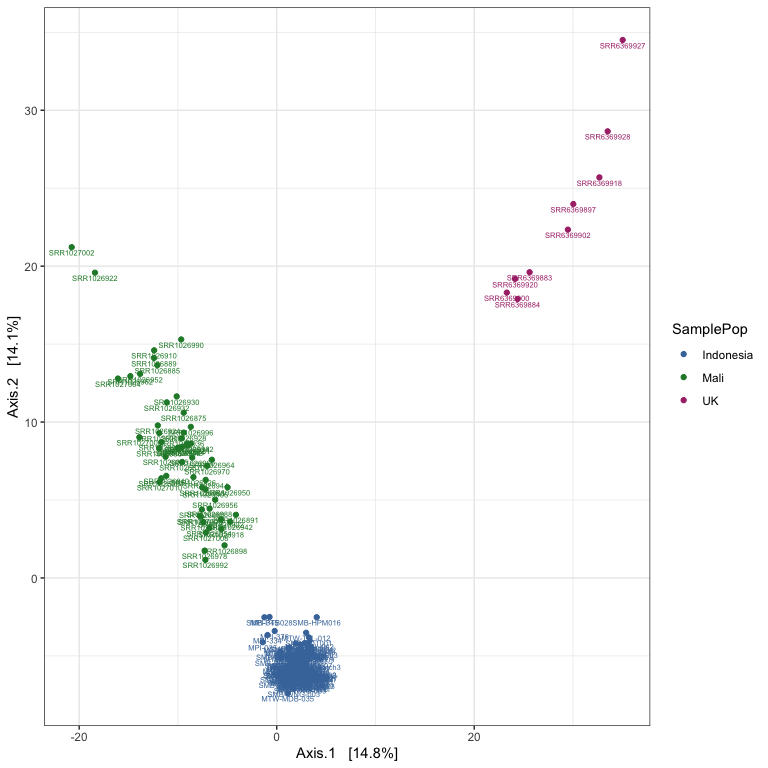
\includegraphics{1.IndonesianVsMaliAndTBControls_CLRMethod_files/figure-latex/unnamed-chunk-18-1} \end{center}

We can see that all populations have a high bacterial load, however in
the Malian and Indonesian dataset, there'a also a high abundance of
Plasmodium and flavivirus. We can also see that the Malian dataset has a
high proportion of reads mapping to archaea.

Now let's check to see how this compares to the rarefied data.

\hypertarget{rarefied-compositional-data}{%
\subsection{Rarefied compositional
data}\label{rarefied-compositional-data}}

One of the most common ways to normalise data is through rarefying, or
subsampling, the entire library to the lowest read depth in the dataset.
Rarefaction is performed by drawing reads without replacement from each
sample so that all samples have the same number of total counts. This
process standardizes the library size across samples and is especially
important for calulating diversity metrics, where read depth influences
microbe diversity.

From what I've found, many people in the microbiomics community have
very strong opinions about rarefying data. Some camps, such as QIIME,
think that it's just fine, whereas others, such as the creators of
Phyloseq, strongly advise against it. A seminal, and of the most
well-referenced papers about the disadvantages of rarefying data, was
published in 2014 by
\href{https://journals.plos.org/ploscompbiol/article?id=10.1371/journal.pcbi.1003531}{McMurdie
\& Holmes}. The arguments they have echo the main concerns seen within
the `anti-rarefy' camps: namely that rarefying data 1) decreases the
ability to detect rare taxa and 2) can lead to unequally-rarefied data
due to rare taxa being over or underrepresented in libraries normalised
to a small size.

Although
\href{https://www.ncbi.nlm.nih.gov/pmc/articles/PMC5335496/}{some
authors} argue that rarefaction is, in fact, a perfectly suitable option
(particularly for small library sizes), I do think this is a valid
point.

Recently, a package called \href{https://peerj.com/articles/9593/}{SRS}
(standing for Scaling with Ranked Subsampling) came out in R and it
preserves OTU frequencies by 1) scaling counts by a constant factor
where the sum of the scaled counts equals the minimum library size
chosen by the user and 2) performing a ranked subsampling on the data.

For this study, I chose Cmin (i.e., the number of counts to which all
samples will be normalized) to 2,000 since a
\href{https://www.pnas.org/content/108/Supplement_1/4516}{seminal paper}
in the microbiome field tested this and found that 2,000 single-end
reads are sufficient for detecting most communities.

SRS won't work if we have samples with a library size under this
threshold, so let's remove all samples under 2000, then perform SRS.

\begin{Shaded}
\begin{Highlighting}[]
\NormalTok{minControl=}\DecValTok{2000}
\NormalTok{keep=}\KeywordTok{names}\NormalTok{(}\KeywordTok{which}\NormalTok{(}\KeywordTok{sample_sums}\NormalTok{(merged_phylo_counts)}\OperatorTok{>=}\NormalTok{minControl))}
\NormalTok{pruned_data=}\KeywordTok{prune_samples}\NormalTok{(keep, merged_phylo_counts)}
\KeywordTok{any}\NormalTok{(}\KeywordTok{taxa_sums}\NormalTok{(pruned_data) }\OperatorTok{==}\StringTok{ }\DecValTok{0}\NormalTok{)}
\end{Highlighting}
\end{Shaded}

\begin{verbatim}
## [1] TRUE
\end{verbatim}

\begin{Shaded}
\begin{Highlighting}[]
\CommentTok{# TRUE}
\NormalTok{pruned_data <-}\StringTok{ }\KeywordTok{prune_taxa}\NormalTok{(}\KeywordTok{taxa_sums}\NormalTok{(pruned_data) }\OperatorTok{>}\StringTok{ }\DecValTok{0}\NormalTok{, pruned_data)}
\KeywordTok{any}\NormalTok{(}\KeywordTok{taxa_sums}\NormalTok{(pruned_data) }\OperatorTok{==}\StringTok{ }\DecValTok{0}\NormalTok{)}
\end{Highlighting}
\end{Shaded}

\begin{verbatim}
## [1] FALSE
\end{verbatim}

\begin{Shaded}
\begin{Highlighting}[]
\CommentTok{# FALSE}
\NormalTok{pruned_data_df=}\KeywordTok{as.data.frame}\NormalTok{(}\KeywordTok{otu_table}\NormalTok{(pruned_data))}
\NormalTok{SRS=}\KeywordTok{SRS}\NormalTok{(pruned_data_df,minControl)}
\KeywordTok{rownames}\NormalTok{(SRS)=}\KeywordTok{rownames}\NormalTok{(pruned_data_df)}

\CommentTok{# transform back into phyloseq object}
\NormalTok{taxa =}\StringTok{ }\KeywordTok{otu_table}\NormalTok{(SRS, }\DataTypeTok{taxa_are_rows =} \OtherTok{TRUE}\NormalTok{)}
\KeywordTok{otu_table}\NormalTok{(pruned_data)=taxa}
\KeywordTok{any}\NormalTok{(}\KeywordTok{taxa_sums}\NormalTok{(pruned_data) }\OperatorTok{==}\StringTok{ }\DecValTok{0}\NormalTok{)}
\end{Highlighting}
\end{Shaded}

\begin{verbatim}
## [1] TRUE
\end{verbatim}

\begin{Shaded}
\begin{Highlighting}[]
\CommentTok{# TRUE}
\NormalTok{pruned_data <-}\StringTok{ }\KeywordTok{prune_taxa}\NormalTok{(}\KeywordTok{taxa_sums}\NormalTok{(pruned_data) }\OperatorTok{>}\StringTok{ }\DecValTok{0}\NormalTok{, pruned_data)}
\KeywordTok{any}\NormalTok{(}\KeywordTok{taxa_sums}\NormalTok{(pruned_data) }\OperatorTok{==}\StringTok{ }\DecValTok{0}\NormalTok{)}
\end{Highlighting}
\end{Shaded}

\begin{verbatim}
## [1] FALSE
\end{verbatim}

\begin{Shaded}
\begin{Highlighting}[]
\CommentTok{# FALSE}
\end{Highlighting}
\end{Shaded}

Now let's make sure the library sizes are the same and see how the OTU
numbers look like between datasets.

\begin{Shaded}
\begin{Highlighting}[]
\NormalTok{SeqDepthPruned =}\StringTok{ }\KeywordTok{sample_sums}\NormalTok{(pruned_data)}
\KeywordTok{sample_data}\NormalTok{(pruned_data)}\OperatorTok{$}\NormalTok{SeqDepthPruned =}\StringTok{ }\NormalTok{SeqDepthPruned}

\CommentTok{# barplot of library sizes}
\KeywordTok{ggplot}\NormalTok{(}\KeywordTok{meta}\NormalTok{(pruned_data), }\KeywordTok{aes}\NormalTok{(SampleName, SeqDepthPruned)) }\OperatorTok{+}\StringTok{ }\KeywordTok{geom_bar}\NormalTok{(}\DataTypeTok{stat =} \StringTok{"identity"}\NormalTok{, }\KeywordTok{aes}\NormalTok{(}\DataTypeTok{fill =}\NormalTok{ SamplePop)) }\OperatorTok{+}
\KeywordTok{scale_fill_manual}\NormalTok{(}\DataTypeTok{values =} \KeywordTok{c}\NormalTok{(IndonesiaCol,MaliCol,UKCol)) }\OperatorTok{+}\StringTok{ }\KeywordTok{rotate_x_text}\NormalTok{()}
\end{Highlighting}
\end{Shaded}

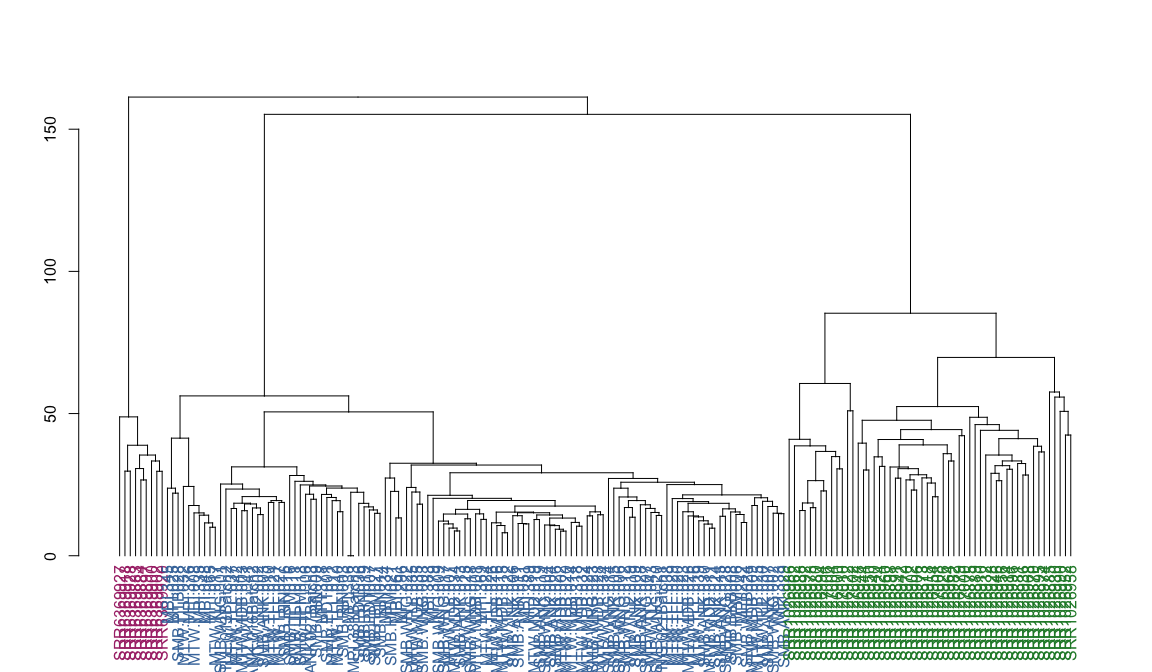
\includegraphics{1.IndonesianVsMaliAndTBControls_CLRMethod_files/figure-latex/unnamed-chunk-20-1.pdf}

\begin{Shaded}
\begin{Highlighting}[]
\CommentTok{# get barplot of total counts per individual}
\NormalTok{nOTUs =}\StringTok{ }\KeywordTok{colSums}\NormalTok{(}\KeywordTok{otu_table}\NormalTok{(pruned_data)}\OperatorTok{!=}\DecValTok{0}\NormalTok{)}
\KeywordTok{sample_data}\NormalTok{(pruned_data)}\OperatorTok{$}\NormalTok{nOTUs =}\StringTok{ }\NormalTok{nOTUs}

\CommentTok{# barplot of OTUs}
\KeywordTok{ggplot}\NormalTok{(}\KeywordTok{meta}\NormalTok{(pruned_data), }\KeywordTok{aes}\NormalTok{(SampleName, nOTUs)) }\OperatorTok{+}\StringTok{ }\KeywordTok{geom_bar}\NormalTok{(}\DataTypeTok{stat =} \StringTok{"identity"}\NormalTok{, }\KeywordTok{aes}\NormalTok{(}\DataTypeTok{fill =}\NormalTok{ SamplePop)) }\OperatorTok{+}
\KeywordTok{scale_fill_manual}\NormalTok{(}\DataTypeTok{values =} \KeywordTok{c}\NormalTok{(IndonesiaCol,MaliCol,UKCol)) }\OperatorTok{+}\StringTok{ }\KeywordTok{rotate_x_text}\NormalTok{()}
\end{Highlighting}
\end{Shaded}

\includegraphics{1.IndonesianVsMaliAndTBControls_CLRMethod_files/figure-latex/unnamed-chunk-20-2.pdf}
Now lets compare the rarefied data to the compositional data.

\begin{Shaded}
\begin{Highlighting}[]
\CommentTok{# add a new column containing family names and superkingdom}
\KeywordTok{tax_table}\NormalTok{(pruned_data)[,}\StringTok{"Superkingdom"}\NormalTok{] =}\StringTok{ }\KeywordTok{paste}\NormalTok{(}\KeywordTok{tax_table}\NormalTok{(pruned_data)[,}\StringTok{"Superkingdom"}\NormalTok{], }\KeywordTok{tax_table}\NormalTok{(pruned_data)[,}\StringTok{"Family"}\NormalTok{], }\DataTypeTok{sep=}\StringTok{"_"}\NormalTok{)}
\KeywordTok{tax_table}\NormalTok{(pruned_data)[,}\StringTok{"Superkingdom"}\NormalTok{] <-}\StringTok{ }\KeywordTok{gsub}\NormalTok{(}\StringTok{"Bacteria_$"}\NormalTok{, }\StringTok{"Bacteria_unclassified"}\NormalTok{, }\KeywordTok{tax_table}\NormalTok{(pruned_data)[,}\StringTok{"Superkingdom"}\NormalTok{])}
\KeywordTok{tax_table}\NormalTok{(pruned_data)[,}\StringTok{"Superkingdom"}\NormalTok{] <-}\StringTok{ }\KeywordTok{gsub}\NormalTok{(}\StringTok{"Eukaryota_$"}\NormalTok{, }\StringTok{"Eukaryota_unclassified"}\NormalTok{, }\KeywordTok{tax_table}\NormalTok{(pruned_data)[,}\StringTok{"Superkingdom"}\NormalTok{])}
\KeywordTok{tax_table}\NormalTok{(pruned_data)[,}\StringTok{"Superkingdom"}\NormalTok{] <-}\StringTok{ }\KeywordTok{gsub}\NormalTok{(}\StringTok{"Viruses_$"}\NormalTok{, }\StringTok{"Viruses_unclassified"}\NormalTok{, }\KeywordTok{tax_table}\NormalTok{(pruned_data)[,}\StringTok{"Superkingdom"}\NormalTok{])}

\CommentTok{# For some reason, top is actually top + 1, so here it would be 20}
\NormalTok{aggregated_phyloCounts <-}\StringTok{ }\KeywordTok{aggregate_top_taxa}\NormalTok{(pruned_data, }\StringTok{"Superkingdom"}\NormalTok{, }\DataTypeTok{top =} \DecValTok{20}\NormalTok{)}
\CommentTok{# transform to relative counts}
\NormalTok{relative_phyloCounts <-}\StringTok{ }\NormalTok{microbiome}\OperatorTok{::}\KeywordTok{transform}\NormalTok{(aggregated_phyloCounts, }\StringTok{"compositional"}\NormalTok{)}
\CommentTok{# Remove weird extra family names added at the end of Superkingdom names}
\KeywordTok{tax_table}\NormalTok{(relative_phyloCounts)[,}\StringTok{"Superkingdom"}\NormalTok{] <-}\StringTok{ }\KeywordTok{paste}\NormalTok{(}\KeywordTok{sapply}\NormalTok{(}\KeywordTok{strsplit}\NormalTok{(}\KeywordTok{taxa_names}\NormalTok{(relative_phyloCounts), }\StringTok{"[_.]"}\NormalTok{), }\StringTok{`}\DataTypeTok{[}\StringTok{`}\NormalTok{, }\DecValTok{1}\NormalTok{), }\KeywordTok{sapply}\NormalTok{(}\KeywordTok{strsplit}\NormalTok{(}\KeywordTok{taxa_names}\NormalTok{(relative_phyloCounts), }\StringTok{"[_.]"}\NormalTok{), }\StringTok{`}\DataTypeTok{[}\StringTok{`}\NormalTok{, }\DecValTok{2}\NormalTok{), }\DataTypeTok{sep=}\StringTok{"_"}\NormalTok{)}
\CommentTok{# Change "Other_NA" to just "Other"}
\KeywordTok{tax_table}\NormalTok{(relative_phyloCounts)[,}\StringTok{"Superkingdom"}\NormalTok{][}\KeywordTok{grep}\NormalTok{(}\StringTok{"Other"}\NormalTok{, }\KeywordTok{taxa_names}\NormalTok{(relative_phyloCounts))] =}\StringTok{ "Other"}

\CommentTok{# Plot}
\NormalTok{p=}\KeywordTok{plot_bar}\NormalTok{(relative_phyloCounts, }\DataTypeTok{fill =} \StringTok{"Superkingdom"}\NormalTok{)}

\CommentTok{# set colour palette}
\NormalTok{families=}\KeywordTok{levels}\NormalTok{(p}\OperatorTok{$}\NormalTok{data}\OperatorTok{$}\NormalTok{Superkingdom)}
\CommentTok{# get number of families in each kingdom}
\KeywordTok{table}\NormalTok{(}\KeywordTok{sapply}\NormalTok{(}\KeywordTok{strsplit}\NormalTok{(families, }\StringTok{"[_.]"}\NormalTok{), }\StringTok{`}\DataTypeTok{[}\StringTok{`}\NormalTok{, }\DecValTok{1}\NormalTok{))}
\end{Highlighting}
\end{Shaded}

\begin{verbatim}
## 
##   Archaea  Bacteria Eukaryota     Other   Viruses 
##         1        13         3         1         3
\end{verbatim}

\begin{Shaded}
\begin{Highlighting}[]
\NormalTok{PaletteArchaea =}\StringTok{ }\KeywordTok{colorRampPalette}\NormalTok{(}\KeywordTok{c}\NormalTok{(}\StringTok{"#DDCC77"}\NormalTok{))(}\DecValTok{1}\NormalTok{)}
\NormalTok{PaletteBacteria =}\StringTok{ }\KeywordTok{colorRampPalette}\NormalTok{(}\KeywordTok{c}\NormalTok{(}\StringTok{"#023858"}\NormalTok{,}\StringTok{"#74a9cf"}\NormalTok{))(}\DecValTok{13}\NormalTok{)}
\NormalTok{PaletteEukaryote =}\StringTok{ }\KeywordTok{colorRampPalette}\NormalTok{(}\KeywordTok{c}\NormalTok{(}\StringTok{"#fd8d3c"}\NormalTok{,}\StringTok{"#800026"}\NormalTok{))(}\DecValTok{3}\NormalTok{)}
\NormalTok{PaletteOther =}\StringTok{ }\KeywordTok{colorRampPalette}\NormalTok{(}\KeywordTok{c}\NormalTok{(}\StringTok{"black"}\NormalTok{))(}\DecValTok{1}\NormalTok{)}
\NormalTok{PaletteVirus =}\StringTok{ }\KeywordTok{colorRampPalette}\NormalTok{(}\KeywordTok{c}\NormalTok{(}\StringTok{"#78c679"}\NormalTok{,}\StringTok{"#006837"}\NormalTok{))(}\DecValTok{3}\NormalTok{)}

\NormalTok{Merged_Palette <-}\StringTok{ }\KeywordTok{c}\NormalTok{(PaletteArchaea,PaletteBacteria,PaletteEukaryote,PaletteOther,PaletteVirus)}

\NormalTok{phyloseq}\OperatorTok{::}\KeywordTok{plot_bar}\NormalTok{(relative_phyloCounts, }\DataTypeTok{fill =} \StringTok{"Superkingdom"}\NormalTok{) }\OperatorTok{+}
\StringTok{  }\KeywordTok{geom_bar}\NormalTok{(}\KeywordTok{aes}\NormalTok{(}\DataTypeTok{fill =}\NormalTok{ Superkingdom), }\DataTypeTok{stat =} \StringTok{"identity"}\NormalTok{, }\DataTypeTok{position =} \StringTok{"stack"}\NormalTok{) }\OperatorTok{+}
\StringTok{  }\KeywordTok{labs}\NormalTok{(}\DataTypeTok{x =} \StringTok{""}\NormalTok{, }\DataTypeTok{y =} \StringTok{"Relative Abundance}\CharTok{\textbackslash{}n}\StringTok{"}\NormalTok{) }\OperatorTok{+}
\StringTok{  }\KeywordTok{facet_wrap}\NormalTok{(}\OperatorTok{~}\StringTok{ }\NormalTok{SamplePop, }\DataTypeTok{scales =} \StringTok{"free"}\NormalTok{) }\OperatorTok{+}\StringTok{ }\KeywordTok{scale_fill_manual}\NormalTok{(}\DataTypeTok{values=}\NormalTok{Merged_Palette) }\OperatorTok{+}
\StringTok{  }\KeywordTok{theme}\NormalTok{(}\DataTypeTok{panel.background =} \KeywordTok{element_blank}\NormalTok{(), }\DataTypeTok{axis.text.x=}\KeywordTok{element_blank}\NormalTok{(), }\DataTypeTok{axis.ticks.x=}\KeywordTok{element_blank}\NormalTok{())}
\end{Highlighting}
\end{Shaded}

\includegraphics{1.IndonesianVsMaliAndTBControls_CLRMethod_files/figure-latex/unnamed-chunk-21-1.pdf}
Although a lot of the samples are missing, the same trend still holds
true- bacteria dominating the UK samples, while apicomplexa, flavivirus,
and archae being dominant in the Indonesian and Malian samples.

\hypertarget{differential-abundance-testing}{%
\section{Differential abundance
testing}\label{differential-abundance-testing}}

We're intersted in testing whether the species composition between
populations is significantly different. Visually, we saw that the
populations look different, but we can't say that for sure. One way to
test this is through differnetial abundance testing.

\begin{Shaded}
\begin{Highlighting}[]
\CommentTok{# Differnetial abundance testing}
\NormalTok{IndoVsUK=}\KeywordTok{subset_samples}\NormalTok{(merged_phylo_counts, SamplePop }\OperatorTok{!=}\StringTok{ "Mali"}\NormalTok{)}
\KeywordTok{any}\NormalTok{(}\KeywordTok{taxa_sums}\NormalTok{(IndoVsUK) }\OperatorTok{==}\StringTok{ }\DecValTok{0}\NormalTok{)}
\end{Highlighting}
\end{Shaded}

\begin{verbatim}
## [1] TRUE
\end{verbatim}

\begin{Shaded}
\begin{Highlighting}[]
\CommentTok{# TRUE}
\NormalTok{IndoVsUK <-}\StringTok{ }\KeywordTok{prune_taxa}\NormalTok{(}\KeywordTok{taxa_sums}\NormalTok{(IndoVsUK) }\OperatorTok{>}\StringTok{ }\DecValTok{0}\NormalTok{, IndoVsUK)}
\KeywordTok{taxa_names}\NormalTok{(IndoVsUK)=}\KeywordTok{make.unique}\NormalTok{(}\KeywordTok{tax_table}\NormalTok{(IndoVsUK)[,}\StringTok{"Family"}\NormalTok{])}
\NormalTok{aldex2_IndoVsUK <-}\StringTok{ }\NormalTok{ALDEx2}\OperatorTok{::}\KeywordTok{aldex}\NormalTok{(}\KeywordTok{data.frame}\NormalTok{(phyloseq}\OperatorTok{::}\KeywordTok{otu_table}\NormalTok{(IndoVsUK)), phyloseq}\OperatorTok{::}\KeywordTok{sample_data}\NormalTok{(IndoVsUK)}\OperatorTok{$}\NormalTok{SamplePop, }\DataTypeTok{test=}\StringTok{"t"}\NormalTok{, }\DataTypeTok{effect =} \OtherTok{TRUE}\NormalTok{)}
\NormalTok{sig_aldex2_IndoVsUK <-}\StringTok{ }\NormalTok{aldex2_IndoVsUK }\OperatorTok
\StringTok{  }\KeywordTok{rownames_to_column}\NormalTok{(}\DataTypeTok{var =} \StringTok{"OTU"}\NormalTok{) }\OperatorTok
\StringTok{  }\KeywordTok{filter}\NormalTok{(wi.eBH }\OperatorTok{<}\StringTok{ }\FloatTok{0.05}\NormalTok{) }\OperatorTok
\StringTok{  }\KeywordTok{arrange}\NormalTok{(effect, wi.eBH) }\OperatorTok
\StringTok{  }\NormalTok{dplyr}\OperatorTok{::}\KeywordTok{select}\NormalTok{(OTU, diff.btw, diff.win, effect, wi.ep, wi.eBH)}
\CommentTok{# set significance colours}
\NormalTok{aldex2_IndoVsUK}\OperatorTok{$}\NormalTok{threshold <-}\StringTok{ }\NormalTok{aldex2_IndoVsUK}\OperatorTok{$}\NormalTok{we.eBH }\OperatorTok{<=}\StringTok{ }\FloatTok{0.05}
\NormalTok{aldex2_IndoVsUK}\OperatorTok{$}\NormalTok{threshold =}\StringTok{ }\KeywordTok{as.numeric}\NormalTok{(aldex2_IndoVsUK}\OperatorTok{$}\NormalTok{threshold) }\OperatorTok{+}\StringTok{ }\DecValTok{1}

\CommentTok{# adjust label names}
\NormalTok{labels =}\StringTok{ }\KeywordTok{sapply}\NormalTok{(}\KeywordTok{strsplit}\NormalTok{(}\KeywordTok{rownames}\NormalTok{(aldex2_IndoVsUK), }\StringTok{"[..]"}\NormalTok{), }\StringTok{`}\DataTypeTok{[}\StringTok{`}\NormalTok{, }\DecValTok{1}\NormalTok{) }\OperatorTok\StringTok{ }\KeywordTok{gsub}\NormalTok{(}\StringTok{"unk_p"}\NormalTok{,}\StringTok{"Fungi"}\NormalTok{,.)}
\NormalTok{taxa_superkingdom =}\StringTok{ }\KeywordTok{sapply}\NormalTok{(}\KeywordTok{strsplit}\NormalTok{(}\KeywordTok{tax_table}\NormalTok{(IndoVsUK)[,}\StringTok{"Superkingdom"}\NormalTok{], }\StringTok{"[_.]"}\NormalTok{), }\StringTok{`}\DataTypeTok{[}\StringTok{`}\NormalTok{, }\DecValTok{1}\NormalTok{) }\OperatorTok\StringTok{ }\KeywordTok{gsub}\NormalTok{(}\StringTok{"unk_p"}\NormalTok{,}\StringTok{"Fungi"}\NormalTok{,.)}

\CommentTok{# plot}
\KeywordTok{ggplot}\NormalTok{(aldex2_IndoVsUK) }\OperatorTok{+}
\StringTok{  }\KeywordTok{geom_point}\NormalTok{(}\KeywordTok{aes}\NormalTok{(}\DataTypeTok{x =}\NormalTok{ effect, }\DataTypeTok{y =} \OperatorTok{-}\KeywordTok{log10}\NormalTok{(wi.eBH)), }\DataTypeTok{color =} \KeywordTok{ifelse}\NormalTok{(aldex2_IndoVsUK}\OperatorTok{$}\NormalTok{wi.eBH }\OperatorTok{<=}\StringTok{ }\FloatTok{0.05}\NormalTok{, }\KeywordTok{c}\NormalTok{(}\StringTok{"grey"}\NormalTok{,}\StringTok{"#023858"}\NormalTok{,}\StringTok{"#800026"}\NormalTok{,}\StringTok{"grey"}\NormalTok{,}\StringTok{"#78c679"}\NormalTok{)[}\KeywordTok{as.numeric}\NormalTok{(}\KeywordTok{as.factor}\NormalTok{(taxa_superkingdom))],}\StringTok{"black"}\NormalTok{), }\DataTypeTok{alpha =} \FloatTok{0.65}\NormalTok{, }\DataTypeTok{size=}\DecValTok{5}\NormalTok{) }\OperatorTok{+}
\StringTok{  }\CommentTok{#geom_text_repel(aes(x = effect, y = -log10(wi.eBH), label = rownames(aldex2_IndoVsDutch))) +}
\StringTok{  }\KeywordTok{geom_text_repel}\NormalTok{(}\KeywordTok{aes}\NormalTok{(}\DataTypeTok{x =}\NormalTok{ effect, }\DataTypeTok{y =} \OperatorTok{-}\KeywordTok{log10}\NormalTok{(wi.eBH), }\DataTypeTok{label =} \KeywordTok{ifelse}\NormalTok{(wi.eBH }\OperatorTok{<=}\StringTok{ }\FloatTok{0.001}\NormalTok{, labels,}\StringTok{""}\NormalTok{))) }\OperatorTok{+}
\StringTok{  }\KeywordTok{ggtitle}\NormalTok{(}\StringTok{"Indonesia Versus UK"}\NormalTok{) }\OperatorTok{+}
\StringTok{  }\KeywordTok{xlab}\NormalTok{(}\StringTok{"effect"}\NormalTok{) }\OperatorTok{+}\StringTok{ }
\StringTok{  }\KeywordTok{ylab}\NormalTok{(}\StringTok{"-log10 adjusted p-value"}\NormalTok{) }\OperatorTok{+}
\StringTok{  }\KeywordTok{theme}\NormalTok{(}\DataTypeTok{legend.position =} \StringTok{"none"}\NormalTok{,}
        \DataTypeTok{plot.title =} \KeywordTok{element_text}\NormalTok{(}\DataTypeTok{size =} \KeywordTok{rel}\NormalTok{(}\FloatTok{1.5}\NormalTok{), }\DataTypeTok{hjust =} \FloatTok{0.5}\NormalTok{),}
        \DataTypeTok{axis.title =} \KeywordTok{element_text}\NormalTok{(}\DataTypeTok{size =} \KeywordTok{rel}\NormalTok{(}\FloatTok{1.25}\NormalTok{)))}
\end{Highlighting}
\end{Shaded}

\begin{center}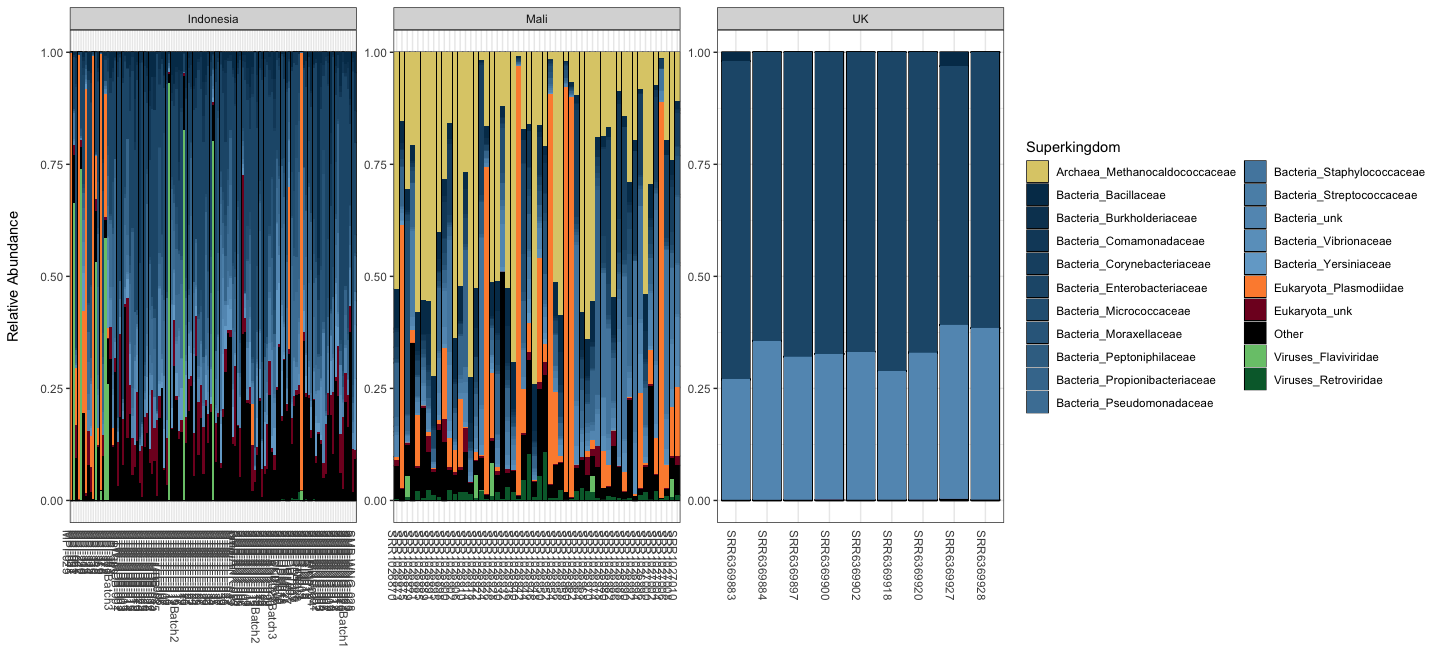
\includegraphics{1.IndonesianVsMaliAndTBControls_CLRMethod_files/figure-latex/unnamed-chunk-22-1} \end{center}

\begin{Shaded}
\begin{Highlighting}[]
\NormalTok{IndoVsMali=}\KeywordTok{subset_samples}\NormalTok{(merged_phylo_counts, SamplePop }\OperatorTok{!=}\StringTok{ "UK"}\NormalTok{)}
\KeywordTok{any}\NormalTok{(}\KeywordTok{taxa_sums}\NormalTok{(IndoVsMali) }\OperatorTok{==}\StringTok{ }\DecValTok{0}\NormalTok{)}
\end{Highlighting}
\end{Shaded}

\begin{verbatim}
## [1] TRUE
\end{verbatim}

\begin{Shaded}
\begin{Highlighting}[]
\CommentTok{# TRUE}
\NormalTok{IndoVsMali <-}\StringTok{ }\KeywordTok{prune_taxa}\NormalTok{(}\KeywordTok{taxa_sums}\NormalTok{(IndoVsMali) }\OperatorTok{>}\StringTok{ }\DecValTok{0}\NormalTok{, IndoVsMali)}
\KeywordTok{taxa_names}\NormalTok{(IndoVsMali)=}\KeywordTok{make.unique}\NormalTok{(}\KeywordTok{tax_table}\NormalTok{(IndoVsMali)[,}\StringTok{"Family"}\NormalTok{])}
\NormalTok{aldex2_IndoVsMali <-}\StringTok{ }\NormalTok{ALDEx2}\OperatorTok{::}\KeywordTok{aldex}\NormalTok{(}\KeywordTok{data.frame}\NormalTok{(phyloseq}\OperatorTok{::}\KeywordTok{otu_table}\NormalTok{(IndoVsMali)), phyloseq}\OperatorTok{::}\KeywordTok{sample_data}\NormalTok{(IndoVsMali)}\OperatorTok{$}\NormalTok{SamplePop, }\DataTypeTok{test=}\StringTok{"t"}\NormalTok{, }\DataTypeTok{effect =} \OtherTok{TRUE}\NormalTok{)}
\NormalTok{sig_aldex2_IndoVsMali <-}\StringTok{ }\NormalTok{aldex2_IndoVsMali }\OperatorTok
\StringTok{  }\KeywordTok{rownames_to_column}\NormalTok{(}\DataTypeTok{var =} \StringTok{"OTU"}\NormalTok{) }\OperatorTok
\StringTok{  }\KeywordTok{filter}\NormalTok{(wi.eBH }\OperatorTok{<}\StringTok{ }\FloatTok{0.05}\NormalTok{) }\OperatorTok
\StringTok{  }\KeywordTok{arrange}\NormalTok{(effect, wi.eBH) }\OperatorTok
\StringTok{  }\NormalTok{dplyr}\OperatorTok{::}\KeywordTok{select}\NormalTok{(OTU, diff.btw, diff.win, effect, wi.ep, wi.eBH)}

\CommentTok{# set significance colours}
\NormalTok{aldex2_IndoVsMali}\OperatorTok{$}\NormalTok{threshold <-}\StringTok{ }\NormalTok{aldex2_IndoVsMali}\OperatorTok{$}\NormalTok{we.eBH }\OperatorTok{<=}\StringTok{ }\FloatTok{0.05}
\NormalTok{aldex2_IndoVsMali}\OperatorTok{$}\NormalTok{threshold =}\StringTok{ }\KeywordTok{as.numeric}\NormalTok{(aldex2_IndoVsMali}\OperatorTok{$}\NormalTok{threshold) }\OperatorTok{+}\StringTok{ }\DecValTok{1}

\CommentTok{# adjust label names}
\NormalTok{labels =}\StringTok{ }\KeywordTok{sapply}\NormalTok{(}\KeywordTok{strsplit}\NormalTok{(}\KeywordTok{rownames}\NormalTok{(aldex2_IndoVsMali), }\StringTok{"[..]"}\NormalTok{), }\StringTok{`}\DataTypeTok{[}\StringTok{`}\NormalTok{, }\DecValTok{1}\NormalTok{) }\OperatorTok\StringTok{ }\KeywordTok{gsub}\NormalTok{(}\StringTok{"unk_f"}\NormalTok{,}\StringTok{"Fungi"}\NormalTok{,.)}
\CommentTok{# plot}
\KeywordTok{ggplot}\NormalTok{(aldex2_IndoVsMali) }\OperatorTok{+}
\StringTok{  }\KeywordTok{geom_point}\NormalTok{(}\KeywordTok{aes}\NormalTok{(}\DataTypeTok{x =}\NormalTok{ effect, }\DataTypeTok{y =} \OperatorTok{-}\KeywordTok{log10}\NormalTok{(wi.eBH)), }\DataTypeTok{color =} \KeywordTok{ifelse}\NormalTok{(aldex2_IndoVsMali}\OperatorTok{$}\NormalTok{wi.eBH }\OperatorTok{<=}\StringTok{ }\FloatTok{0.05}\NormalTok{, }\KeywordTok{c}\NormalTok{(}\StringTok{"grey"}\NormalTok{,}\StringTok{"#023858"}\NormalTok{,}\StringTok{"#800026"}\NormalTok{,}\StringTok{"grey"}\NormalTok{,}\StringTok{"#78c679"}\NormalTok{)[}\KeywordTok{as.numeric}\NormalTok{(}\KeywordTok{as.factor}\NormalTok{(}\KeywordTok{tax_table}\NormalTok{(IndoVsMali)[,}\StringTok{"Superkingdom"}\NormalTok{]))],}\StringTok{"black"}\NormalTok{), }\DataTypeTok{alpha =} \FloatTok{0.65}\NormalTok{, }\DataTypeTok{size=}\DecValTok{5}\NormalTok{) }\OperatorTok{+}
\StringTok{  }\KeywordTok{geom_text_repel}\NormalTok{(}\KeywordTok{aes}\NormalTok{(}\DataTypeTok{x =}\NormalTok{ effect, }\DataTypeTok{y =} \OperatorTok{-}\KeywordTok{log10}\NormalTok{(wi.eBH), }\DataTypeTok{label =} \KeywordTok{ifelse}\NormalTok{(wi.eBH }\OperatorTok{<=}\StringTok{ }\FloatTok{0.001}\NormalTok{, labels,}\StringTok{""}\NormalTok{))) }\OperatorTok{+}
\StringTok{  }\CommentTok{#geom_text_repel(aes(x = effect, y = -log10(wi.eBH), label = ifelse(wi.eBH <= 0.001, labels,""))) +}
\StringTok{  }\KeywordTok{ggtitle}\NormalTok{(}\StringTok{"Indonesia Versus Mali"}\NormalTok{) }\OperatorTok{+}
\StringTok{  }\KeywordTok{xlab}\NormalTok{(}\StringTok{"effect"}\NormalTok{) }\OperatorTok{+}\StringTok{ }
\StringTok{  }\KeywordTok{ylab}\NormalTok{(}\StringTok{"-log10 adjusted p-value"}\NormalTok{) }\OperatorTok{+}
\StringTok{  }\KeywordTok{theme}\NormalTok{(}\DataTypeTok{legend.position =} \StringTok{"none"}\NormalTok{,}
        \DataTypeTok{plot.title =} \KeywordTok{element_text}\NormalTok{(}\DataTypeTok{size =} \KeywordTok{rel}\NormalTok{(}\FloatTok{1.5}\NormalTok{), }\DataTypeTok{hjust =} \FloatTok{0.5}\NormalTok{),}
        \DataTypeTok{axis.title =} \KeywordTok{element_text}\NormalTok{(}\DataTypeTok{size =} \KeywordTok{rel}\NormalTok{(}\FloatTok{1.25}\NormalTok{)))}
\end{Highlighting}
\end{Shaded}

\begin{verbatim}
## Warning: Removed 53 rows containing missing values (geom_point).
\end{verbatim}

\begin{center}\includegraphics{1.IndonesianVsMaliAndTBControls_CLRMethod_files/figure-latex/unnamed-chunk-22-2} \end{center}

\hypertarget{alpha-diversity}{%
\section{Alpha diversity}\label{alpha-diversity}}

Alpha diversity measures within-sample diverity and looks at how many
taxa are observed, as well as how evenly they are distributed.

There is a lot of controversy around how best to analyse alpha
diversity. Because a higher sequencing depth will lead to a greater
likelihood of diversity, many people rarefy their data beforehand.
However, rarefying data (as pointed out above), not only discards data,
but leads to biases when rarefied.

Current tools to estimate alpha diversity either underestimate richness
or underestimate uncertainty, however DivNet is a package that adresses
these problems. Divnet is a method for estimating within- and
between-community diversity in ecosystems where taxa interact via an
ecological network. It accounts for differences in sequencing depth and
estimates the number of missing species based on the sequence depth and
number of rare taxa in the data.

To use DivNet, you need unsubsampled data without removing singletons.

\begin{Shaded}
\begin{Highlighting}[]
\CommentTok{# Get phyloseq object without singletons by merging original phyloseq objects}
\NormalTok{merged_phylo_counts_withSingletons <-}\StringTok{ }\KeywordTok{merge_phyloseq}\NormalTok{(AllREadsSE_Indo_Counts_physeq, Mali_Counts_physeq, European_Counts_physeq)}
\CommentTok{# Remove Viridiplantae and Metazoa}
\NormalTok{merged_phylo_counts_withSingletons <-}\StringTok{ }\KeywordTok{subset_taxa}\NormalTok{(merged_phylo_counts_withSingletons, (Kingdom}\OperatorTok{!=}\StringTok{"Viridiplantae"}\NormalTok{))}
\NormalTok{merged_phylo_counts_withSingletons <-}\StringTok{ }\KeywordTok{subset_taxa}\NormalTok{(merged_phylo_counts_withSingletons, (Kingdom}\OperatorTok{!=}\StringTok{"Metazoa"}\NormalTok{))}
\CommentTok{# remove any empty rows}
\NormalTok{merged_phylo_counts_withSingletons <-}\StringTok{ }\KeywordTok{prune_taxa}\NormalTok{(}\KeywordTok{taxa_sums}\NormalTok{(merged_phylo_counts_withSingletons) }\OperatorTok{>}\StringTok{ }\DecValTok{0}\NormalTok{, merged_phylo_counts_withSingletons)}
\end{Highlighting}
\end{Shaded}

Now that we have data without singletons, we now need to merge our data
at a specified taxonomic level. DivNet is computationally expensive, and
therefore a higher level is much, much faster. We'll therefore test how
our groups look like at the Phylum level. Then, we'll run DivNet without
specifying any hypothesis testing.

\begin{Shaded}
\begin{Highlighting}[]
\CommentTok{# comparing diversity at the phylum level}
\NormalTok{pop_comparison <-}\StringTok{ }\NormalTok{merged_phylo_counts_withSingletons }\OperatorTok
\StringTok{  }\KeywordTok{tax_glom}\NormalTok{(}\StringTok{"Phylum"}\NormalTok{)}

\CommentTok{# If we don't change the sample names here from hyphens to periods, we'll get an error later}
\KeywordTok{sample_names}\NormalTok{(pop_comparison) <-}\StringTok{ }\KeywordTok{gsub}\NormalTok{(}\StringTok{"}\CharTok{\textbackslash{}\textbackslash{}}\StringTok{-"}\NormalTok{, }\StringTok{"."}\NormalTok{, }\KeywordTok{sample_names}\NormalTok{(pop_comparison))}

\CommentTok{# Run divnet without specifying any hypothesis testing}
\NormalTok{dv_pop_comparison <-}\StringTok{ }\KeywordTok{divnet}\NormalTok{(pop_comparison, }\DataTypeTok{ncores =} \DecValTok{4}\NormalTok{)}
\end{Highlighting}
\end{Shaded}

\begin{verbatim}
##   |                                                                              |                                                                      |   0%
\end{verbatim}

\begin{verbatim}
## Warning in MCmat(Y = Y_p, W = W, eY = eY, N = N, Q = Q, base = base, sigma =
## sigma, : Running in series; one of the packages doParallel, foreach or doSNOW is
## missing
\end{verbatim}

\begin{verbatim}
##   |                                                                              |============                                                          |  17%
\end{verbatim}

\begin{verbatim}
## Warning in MCmat(Y = Y_p, W = W, eY = eY, N = N, Q = Q, base = base, sigma =
## sigma, : Running in series; one of the packages doParallel, foreach or doSNOW is
## missing
\end{verbatim}

\begin{verbatim}
##   |                                                                              |=======================                                               |  33%
\end{verbatim}

\begin{verbatim}
## Warning in MCmat(Y = Y_p, W = W, eY = eY, N = N, Q = Q, base = base, sigma =
## sigma, : Running in series; one of the packages doParallel, foreach or doSNOW is
## missing
\end{verbatim}

\begin{verbatim}
##   |                                                                              |===================================                                   |  50%
\end{verbatim}

\begin{verbatim}
## Warning in MCmat(Y = Y_p, W = W, eY = eY, N = N, Q = Q, base = base, sigma =
## sigma, : Running in series; one of the packages doParallel, foreach or doSNOW is
## missing
\end{verbatim}

\begin{verbatim}
##   |                                                                              |===============================================                       |  67%
\end{verbatim}

\begin{verbatim}
## Warning in MCmat(Y = Y_p, W = W, eY = eY, N = N, Q = Q, base = base, sigma =
## sigma, : Running in series; one of the packages doParallel, foreach or doSNOW is
## missing
\end{verbatim}

\begin{verbatim}
##   |                                                                              |==========================================================            |  83%
\end{verbatim}

\begin{verbatim}
## Warning in MCmat(Y = Y_p, W = W, eY = eY, N = N, Q = Q, base = base, sigma =
## sigma, : Running in series; one of the packages doParallel, foreach or doSNOW is
## missing
\end{verbatim}

\begin{verbatim}
##   |                                                                              |======================================================================| 100%
##   |                                                                              |                                                                      |   0%
\end{verbatim}

\begin{verbatim}
## Warning in MCmat(Y = Y_p, W = W, eY = eY, N = N, Q = Q, base = base, sigma =
## sigma, : Running in series; one of the packages doParallel, foreach or doSNOW is
## missing
\end{verbatim}

\begin{verbatim}
##   |                                                                              |============                                                          |  17%
\end{verbatim}

\begin{verbatim}
## Warning in MCmat(Y = Y_p, W = W, eY = eY, N = N, Q = Q, base = base, sigma =
## sigma, : Running in series; one of the packages doParallel, foreach or doSNOW is
## missing
\end{verbatim}

\begin{verbatim}
##   |                                                                              |=======================                                               |  33%
\end{verbatim}

\begin{verbatim}
## Warning in MCmat(Y = Y_p, W = W, eY = eY, N = N, Q = Q, base = base, sigma =
## sigma, : Running in series; one of the packages doParallel, foreach or doSNOW is
## missing
\end{verbatim}

\begin{verbatim}
##   |                                                                              |===================================                                   |  50%
\end{verbatim}

\begin{verbatim}
## Warning in MCmat(Y = Y_p, W = W, eY = eY, N = N, Q = Q, base = base, sigma =
## sigma, : Running in series; one of the packages doParallel, foreach or doSNOW is
## missing
\end{verbatim}

\begin{verbatim}
##   |                                                                              |===============================================                       |  67%
\end{verbatim}

\begin{verbatim}
## Warning in MCmat(Y = Y_p, W = W, eY = eY, N = N, Q = Q, base = base, sigma =
## sigma, : Running in series; one of the packages doParallel, foreach or doSNOW is
## missing
\end{verbatim}

\begin{verbatim}
##   |                                                                              |==========================================================            |  83%
\end{verbatim}

\begin{verbatim}
## Warning in MCmat(Y = Y_p, W = W, eY = eY, N = N, Q = Q, base = base, sigma =
## sigma, : Running in series; one of the packages doParallel, foreach or doSNOW is
## missing
\end{verbatim}

\begin{verbatim}
##   |                                                                              |======================================================================| 100%
##   |                                                                              |                                                                      |   0%
\end{verbatim}

\begin{verbatim}
## Warning in MCmat(Y = Y_p, W = W, eY = eY, N = N, Q = Q, base = base, sigma =
## sigma, : Running in series; one of the packages doParallel, foreach or doSNOW is
## missing
\end{verbatim}

\begin{verbatim}
##   |                                                                              |============                                                          |  17%
\end{verbatim}

\begin{verbatim}
## Warning in MCmat(Y = Y_p, W = W, eY = eY, N = N, Q = Q, base = base, sigma =
## sigma, : Running in series; one of the packages doParallel, foreach or doSNOW is
## missing
\end{verbatim}

\begin{verbatim}
##   |                                                                              |=======================                                               |  33%
\end{verbatim}

\begin{verbatim}
## Warning in MCmat(Y = Y_p, W = W, eY = eY, N = N, Q = Q, base = base, sigma =
## sigma, : Running in series; one of the packages doParallel, foreach or doSNOW is
## missing
\end{verbatim}

\begin{verbatim}
##   |                                                                              |===================================                                   |  50%
\end{verbatim}

\begin{verbatim}
## Warning in MCmat(Y = Y_p, W = W, eY = eY, N = N, Q = Q, base = base, sigma =
## sigma, : Running in series; one of the packages doParallel, foreach or doSNOW is
## missing
\end{verbatim}

\begin{verbatim}
##   |                                                                              |===============================================                       |  67%
\end{verbatim}

\begin{verbatim}
## Warning in MCmat(Y = Y_p, W = W, eY = eY, N = N, Q = Q, base = base, sigma =
## sigma, : Running in series; one of the packages doParallel, foreach or doSNOW is
## missing
\end{verbatim}

\begin{verbatim}
##   |                                                                              |==========================================================            |  83%
\end{verbatim}

\begin{verbatim}
## Warning in MCmat(Y = Y_p, W = W, eY = eY, N = N, Q = Q, base = base, sigma =
## sigma, : Running in series; one of the packages doParallel, foreach or doSNOW is
## missing
\end{verbatim}

\begin{verbatim}
##   |                                                                              |======================================================================| 100%
##   |                                                                              |                                                                      |   0%
\end{verbatim}

\begin{verbatim}
## Warning in MCmat(Y = Y_p, W = W, eY = eY, N = N, Q = Q, base = base, sigma =
## sigma, : Running in series; one of the packages doParallel, foreach or doSNOW is
## missing
\end{verbatim}

\begin{verbatim}
##   |                                                                              |============                                                          |  17%
\end{verbatim}

\begin{verbatim}
## Warning in MCmat(Y = Y_p, W = W, eY = eY, N = N, Q = Q, base = base, sigma =
## sigma, : Running in series; one of the packages doParallel, foreach or doSNOW is
## missing
\end{verbatim}

\begin{verbatim}
##   |                                                                              |=======================                                               |  33%
\end{verbatim}

\begin{verbatim}
## Warning in MCmat(Y = Y_p, W = W, eY = eY, N = N, Q = Q, base = base, sigma =
## sigma, : Running in series; one of the packages doParallel, foreach or doSNOW is
## missing
\end{verbatim}

\begin{verbatim}
##   |                                                                              |===================================                                   |  50%
\end{verbatim}

\begin{verbatim}
## Warning in MCmat(Y = Y_p, W = W, eY = eY, N = N, Q = Q, base = base, sigma =
## sigma, : Running in series; one of the packages doParallel, foreach or doSNOW is
## missing
\end{verbatim}

\begin{verbatim}
##   |                                                                              |===============================================                       |  67%
\end{verbatim}

\begin{verbatim}
## Warning in MCmat(Y = Y_p, W = W, eY = eY, N = N, Q = Q, base = base, sigma =
## sigma, : Running in series; one of the packages doParallel, foreach or doSNOW is
## missing
\end{verbatim}

\begin{verbatim}
##   |                                                                              |==========================================================            |  83%
\end{verbatim}

\begin{verbatim}
## Warning in MCmat(Y = Y_p, W = W, eY = eY, N = N, Q = Q, base = base, sigma =
## sigma, : Running in series; one of the packages doParallel, foreach or doSNOW is
## missing
\end{verbatim}

\begin{verbatim}
##   |                                                                              |======================================================================| 100%
##   |                                                                              |                                                                      |   0%
\end{verbatim}

\begin{verbatim}
## Warning in MCmat(Y = Y_p, W = W, eY = eY, N = N, Q = Q, base = base, sigma =
## sigma, : Running in series; one of the packages doParallel, foreach or doSNOW is
## missing
\end{verbatim}

\begin{verbatim}
##   |                                                                              |============                                                          |  17%
\end{verbatim}

\begin{verbatim}
## Warning in MCmat(Y = Y_p, W = W, eY = eY, N = N, Q = Q, base = base, sigma =
## sigma, : Running in series; one of the packages doParallel, foreach or doSNOW is
## missing
\end{verbatim}

\begin{verbatim}
##   |                                                                              |=======================                                               |  33%
\end{verbatim}

\begin{verbatim}
## Warning in MCmat(Y = Y_p, W = W, eY = eY, N = N, Q = Q, base = base, sigma =
## sigma, : Running in series; one of the packages doParallel, foreach or doSNOW is
## missing
\end{verbatim}

\begin{verbatim}
##   |                                                                              |===================================                                   |  50%
\end{verbatim}

\begin{verbatim}
## Warning in MCmat(Y = Y_p, W = W, eY = eY, N = N, Q = Q, base = base, sigma =
## sigma, : Running in series; one of the packages doParallel, foreach or doSNOW is
## missing
\end{verbatim}

\begin{verbatim}
##   |                                                                              |===============================================                       |  67%
\end{verbatim}

\begin{verbatim}
## Warning in MCmat(Y = Y_p, W = W, eY = eY, N = N, Q = Q, base = base, sigma =
## sigma, : Running in series; one of the packages doParallel, foreach or doSNOW is
## missing
\end{verbatim}

\begin{verbatim}
##   |                                                                              |==========================================================            |  83%
\end{verbatim}

\begin{verbatim}
## Warning in MCmat(Y = Y_p, W = W, eY = eY, N = N, Q = Q, base = base, sigma =
## sigma, : Running in series; one of the packages doParallel, foreach or doSNOW is
## missing
\end{verbatim}

\begin{verbatim}
##   |                                                                              |======================================================================| 100%
##   |                                                                              |                                                                      |   0%
\end{verbatim}

\begin{verbatim}
## Warning in MCmat(Y = Y_p, W = W, eY = eY, N = N, Q = Q, base = base, sigma =
## sigma, : Running in series; one of the packages doParallel, foreach or doSNOW is
## missing
\end{verbatim}

\begin{verbatim}
##   |                                                                              |============                                                          |  17%
\end{verbatim}

\begin{verbatim}
## Warning in MCmat(Y = Y_p, W = W, eY = eY, N = N, Q = Q, base = base, sigma =
## sigma, : Running in series; one of the packages doParallel, foreach or doSNOW is
## missing
\end{verbatim}

\begin{verbatim}
##   |                                                                              |=======================                                               |  33%
\end{verbatim}

\begin{verbatim}
## Warning in MCmat(Y = Y_p, W = W, eY = eY, N = N, Q = Q, base = base, sigma =
## sigma, : Running in series; one of the packages doParallel, foreach or doSNOW is
## missing
\end{verbatim}

\begin{verbatim}
##   |                                                                              |===================================                                   |  50%
\end{verbatim}

\begin{verbatim}
## Warning in MCmat(Y = Y_p, W = W, eY = eY, N = N, Q = Q, base = base, sigma =
## sigma, : Running in series; one of the packages doParallel, foreach or doSNOW is
## missing
\end{verbatim}

\begin{verbatim}
##   |                                                                              |===============================================                       |  67%
\end{verbatim}

\begin{verbatim}
## Warning in MCmat(Y = Y_p, W = W, eY = eY, N = N, Q = Q, base = base, sigma =
## sigma, : Running in series; one of the packages doParallel, foreach or doSNOW is
## missing
\end{verbatim}

\begin{verbatim}
##   |                                                                              |==========================================================            |  83%
\end{verbatim}

\begin{verbatim}
## Warning in MCmat(Y = Y_p, W = W, eY = eY, N = N, Q = Q, base = base, sigma =
## sigma, : Running in series; one of the packages doParallel, foreach or doSNOW is
## missing
\end{verbatim}

\begin{verbatim}
##   |                                                                              |======================================================================| 100%
\end{verbatim}

\begin{Shaded}
\begin{Highlighting}[]
\CommentTok{# DivNet outputs a list of the estimates shannon, simpson (alpha diversity)}
\CommentTok{# bray-curtis, euclidean (beta diversity)}
\NormalTok{dv_pop_comparison }\OperatorTok\StringTok{ }\NormalTok{names}
\end{Highlighting}
\end{Shaded}

\begin{verbatim}
##  [1] "shannon"              "simpson"              "bray-curtis"         
##  [4] "euclidean"            "shannon-variance"     "simpson-variance"    
##  [7] "bray-curtis-variance" "euclidean-variance"   "X"                   
## [10] "fitted_z"
\end{verbatim}

DivNet will output an object with estimates for multiple different alpha
(and beta) diversity measures (we'll get to the beta diversity estimates
later). The Shannon and Simpson index are two popular alpha diversity
indices to measure species richness. For Shannon diversity, the
importance of rare taxa are downeighted, since they do not play a large
role in the community or they could potentially be due to error. For
this reason, the Shannon index is one of the most popular alpha
diversity metrics.

To interpret the index, a higher Shannon index means higher diversity,
whereas a lowed index number means lower diversity.

Let's take out the Shannon diversity metric from DivNet and plot it.

\begin{Shaded}
\begin{Highlighting}[]
\CommentTok{# Now let's plot the results of shannon and Simpson diversity}
\NormalTok{summary_df_shannon <-}\StringTok{ }\KeywordTok{as.data.frame}\NormalTok{(dv_pop_comparison}\OperatorTok{$}\NormalTok{shannon }\OperatorTok
\StringTok{  }\NormalTok{summary }\OperatorTok
\StringTok{  }\KeywordTok{add_column}\NormalTok{(}\StringTok{"SampleNames"}\NormalTok{ =}\StringTok{ }\NormalTok{pop_comparison }\OperatorTok\StringTok{ }\NormalTok{otu_table }\OperatorTok\StringTok{ }\NormalTok{sample_names) }\OperatorTok
\StringTok{  }\KeywordTok{add_column}\NormalTok{(}\StringTok{"SamplePop"}\NormalTok{ =}\StringTok{  }\NormalTok{pop_comparison }\OperatorTok\StringTok{ }\NormalTok{sample_data }\OperatorTok\StringTok{ }\NormalTok{.[,}\StringTok{"SamplePop"}\NormalTok{] }\OperatorTok\StringTok{ }\KeywordTok{as.matrix}\NormalTok{(.) }\OperatorTok\StringTok{ }\NormalTok{.[,}\DecValTok{1}\NormalTok{] }\OperatorTok\StringTok{ }\KeywordTok{unname}\NormalTok{(.)))}

\KeywordTok{ggplot}\NormalTok{(summary_df_shannon, }\KeywordTok{aes}\NormalTok{(}\DataTypeTok{y =}\NormalTok{ estimate, }\DataTypeTok{x =}\NormalTok{ SamplePop, }\DataTypeTok{fill =}\NormalTok{ SamplePop)) }\OperatorTok{+}\StringTok{ }\KeywordTok{geom_violin}\NormalTok{(}\DataTypeTok{alpha=}\FloatTok{0.7}\NormalTok{) }\OperatorTok{+}\StringTok{ }
\StringTok{  }\KeywordTok{geom_jitter}\NormalTok{(}\DataTypeTok{height =} \DecValTok{0}\NormalTok{, }\DataTypeTok{width =} \FloatTok{.2}\NormalTok{) }\OperatorTok{+}\StringTok{ }\KeywordTok{geom_boxplot}\NormalTok{(}\DataTypeTok{width=}\FloatTok{0.08}\NormalTok{, }\DataTypeTok{outlier.color =} \OtherTok{NA}\NormalTok{) }\OperatorTok{+}
\StringTok{  }\KeywordTok{scale_fill_manual}\NormalTok{(}\DataTypeTok{values=}\KeywordTok{c}\NormalTok{(IndonesiaCol,MaliCol,UKCol)) }\OperatorTok{+}\StringTok{ }\KeywordTok{ggtitle}\NormalTok{(}\StringTok{"Shannon Diversity"}\NormalTok{) }\OperatorTok{+}
\StringTok{  }\KeywordTok{ylab}\NormalTok{(}\StringTok{"Estimate of Shannon Diversity"}\NormalTok{)}
\end{Highlighting}
\end{Shaded}

\begin{center}\includegraphics{1.IndonesianVsMaliAndTBControls_CLRMethod_files/figure-latex/unnamed-chunk-25-1} \end{center}

We can see that the Malian samples, on average, have the highest
estimates of Shannon alpha diversity, followed by the Indonesian
population, then the UK population.

We can also plot each individual sample, along with their standard
deviation (another cool, and imprortant feature that DivNet calculates
and uses in their hypothesis testing).

\begin{Shaded}
\begin{Highlighting}[]
\KeywordTok{plot}\NormalTok{(dv_pop_comparison}\OperatorTok{$}\NormalTok{shannon, pop_comparison, }\DataTypeTok{col =} \StringTok{"SamplePop"}\NormalTok{) }\OperatorTok{+}\StringTok{ }\KeywordTok{scale_colour_manual}\NormalTok{(}\DataTypeTok{values=}\KeywordTok{c}\NormalTok{(IndonesiaCol,MaliCol,UKCol))}
\end{Highlighting}
\end{Shaded}

\begin{center}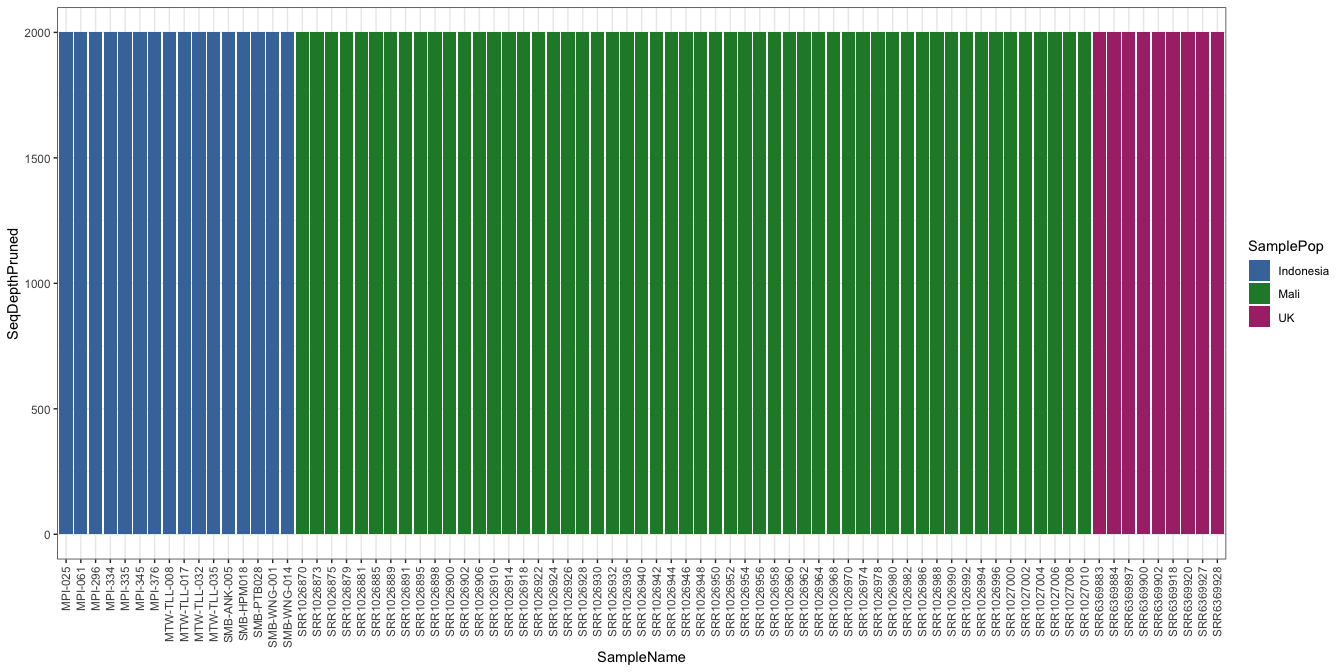
\includegraphics{1.IndonesianVsMaliAndTBControls_CLRMethod_files/figure-latex/unnamed-chunk-26-1} \end{center}

We can see that the Indonesian samples have the highest amount of SE
around their estimates, but this makes sense given that this is the
population with the lowest library size.

Now let's use see how the population diversity looks like when we use
the Simpson diversity. The Simpson diversity index is a similarity index
where the higher the value, the lower the diversity. It measures the
probability that two individuals randomly selected from a sample will
belong to the same species. With this index, 0 represents infinite
diversity and 1, no diversity.

\begin{Shaded}
\begin{Highlighting}[]
\NormalTok{summary_df_simpson <-}\StringTok{ }\KeywordTok{as.data.frame}\NormalTok{(dv_pop_comparison}\OperatorTok{$}\NormalTok{simpson }\OperatorTok
\StringTok{  }\NormalTok{summary }\OperatorTok
\StringTok{  }\KeywordTok{add_column}\NormalTok{(}\StringTok{"SampleNames"}\NormalTok{ =}\StringTok{ }\NormalTok{pop_comparison }\OperatorTok\StringTok{ }\NormalTok{otu_table }\OperatorTok\StringTok{ }\NormalTok{sample_names) }\OperatorTok
\StringTok{  }\KeywordTok{add_column}\NormalTok{(}\StringTok{"SamplePop"}\NormalTok{ =}\StringTok{  }\NormalTok{pop_comparison }\OperatorTok\StringTok{ }\NormalTok{sample_data }\OperatorTok\StringTok{ }\NormalTok{.[,}\StringTok{"SamplePop"}\NormalTok{] }\OperatorTok\StringTok{ }\KeywordTok{as.matrix}\NormalTok{(.) }\OperatorTok\StringTok{ }\NormalTok{.[,}\DecValTok{1}\NormalTok{] }\OperatorTok\StringTok{ }\KeywordTok{unname}\NormalTok{(.)))}

\KeywordTok{ggplot}\NormalTok{(summary_df_simpson, }\KeywordTok{aes}\NormalTok{(}\DataTypeTok{y =}\NormalTok{ estimate, }\DataTypeTok{x =}\NormalTok{ SamplePop, }\DataTypeTok{fill =}\NormalTok{ SamplePop)) }\OperatorTok{+}\StringTok{ }\KeywordTok{geom_violin}\NormalTok{(}\DataTypeTok{alpha=}\FloatTok{0.7}\NormalTok{) }\OperatorTok{+}\StringTok{ }
\StringTok{  }\KeywordTok{geom_jitter}\NormalTok{(}\DataTypeTok{height =} \DecValTok{0}\NormalTok{, }\DataTypeTok{width =} \FloatTok{.2}\NormalTok{) }\OperatorTok{+}\StringTok{ }\KeywordTok{geom_boxplot}\NormalTok{(}\DataTypeTok{width=}\FloatTok{0.08}\NormalTok{, }\DataTypeTok{outlier.color =} \OtherTok{NA}\NormalTok{) }\OperatorTok{+}
\StringTok{  }\KeywordTok{scale_fill_manual}\NormalTok{(}\DataTypeTok{values=}\KeywordTok{c}\NormalTok{(IndonesiaCol,MaliCol,UKCol)) }\OperatorTok{+}\StringTok{ }\KeywordTok{ggtitle}\NormalTok{(}\StringTok{"Simpson's Diversity Index"}\NormalTok{) }\OperatorTok{+}
\StringTok{  }\KeywordTok{ylab}\NormalTok{(}\StringTok{"Estimate of Simpson Diversity"}\NormalTok{)}
\end{Highlighting}
\end{Shaded}

\begin{center}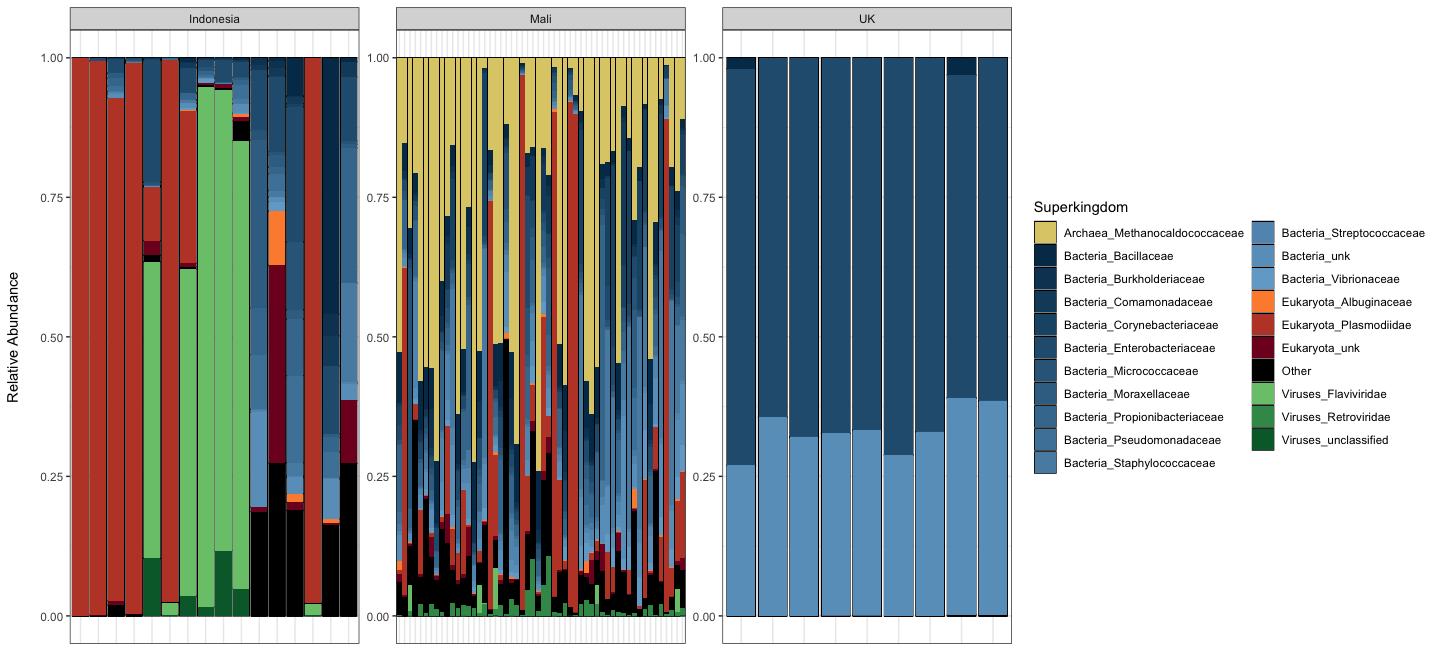
\includegraphics{1.IndonesianVsMaliAndTBControls_CLRMethod_files/figure-latex/unnamed-chunk-27-1} \end{center}

Again, we can see that the Malian population has the highest diversity
(remember, and index of 0 equates to infinite diversity), while the UK
population has the lowest diversity.

This is how the diversity looks like with SE included for each sample.

\begin{Shaded}
\begin{Highlighting}[]
\KeywordTok{plot}\NormalTok{(dv_pop_comparison}\OperatorTok{$}\NormalTok{simpson, pop_comparison, }\DataTypeTok{col =} \StringTok{"SamplePop"}\NormalTok{) }\OperatorTok{+}\StringTok{ }\KeywordTok{scale_colour_manual}\NormalTok{(}\DataTypeTok{values=}\KeywordTok{c}\NormalTok{(IndonesiaCol,MaliCol,UKCol))}
\end{Highlighting}
\end{Shaded}

\begin{center}\includegraphics{1.IndonesianVsMaliAndTBControls_CLRMethod_files/figure-latex/unnamed-chunk-28-1} \end{center}

Since a larger Simpson index value equates to a lower diversity index,
many people find this confusing and not very intuitive. Therefore, the
inverse Simpsone Index, or 1 - Simpson Index, is also commonly used.
Let's plot that now.

\begin{Shaded}
\begin{Highlighting}[]
\CommentTok{# Subtract the Simpson estimate from one}
\NormalTok{summary_df_simpson}\OperatorTok{$}\NormalTok{estimate =}\StringTok{ }\DecValTok{1}\OperatorTok{-}\NormalTok{summary_df_simpson}\OperatorTok{$}\NormalTok{estimate}
\CommentTok{# Plot}
\KeywordTok{ggplot}\NormalTok{(summary_df_simpson, }\KeywordTok{aes}\NormalTok{(}\DataTypeTok{y =}\NormalTok{ estimate, }\DataTypeTok{x =}\NormalTok{ SamplePop, }\DataTypeTok{fill =}\NormalTok{ SamplePop)) }\OperatorTok{+}\StringTok{ }\KeywordTok{geom_violin}\NormalTok{(}\DataTypeTok{alpha=}\FloatTok{0.7}\NormalTok{) }\OperatorTok{+}\StringTok{ }
\StringTok{  }\KeywordTok{geom_jitter}\NormalTok{(}\DataTypeTok{height =} \DecValTok{0}\NormalTok{, }\DataTypeTok{width =} \FloatTok{.2}\NormalTok{) }\OperatorTok{+}\StringTok{ }\KeywordTok{geom_boxplot}\NormalTok{(}\DataTypeTok{width=}\FloatTok{0.08}\NormalTok{, }\DataTypeTok{outlier.color =} \OtherTok{NA}\NormalTok{) }\OperatorTok{+}
\StringTok{  }\KeywordTok{scale_fill_manual}\NormalTok{(}\DataTypeTok{values=}\KeywordTok{c}\NormalTok{(IndonesiaCol,MaliCol,UKCol)) }\OperatorTok{+}\StringTok{ }\KeywordTok{ggtitle}\NormalTok{(}\StringTok{"Simpson's Diversity Index"}\NormalTok{) }\OperatorTok{+}
\StringTok{  }\KeywordTok{ylab}\NormalTok{(}\StringTok{"Estimate of Simpson Diversity"}\NormalTok{)}
\end{Highlighting}
\end{Shaded}

\begin{center}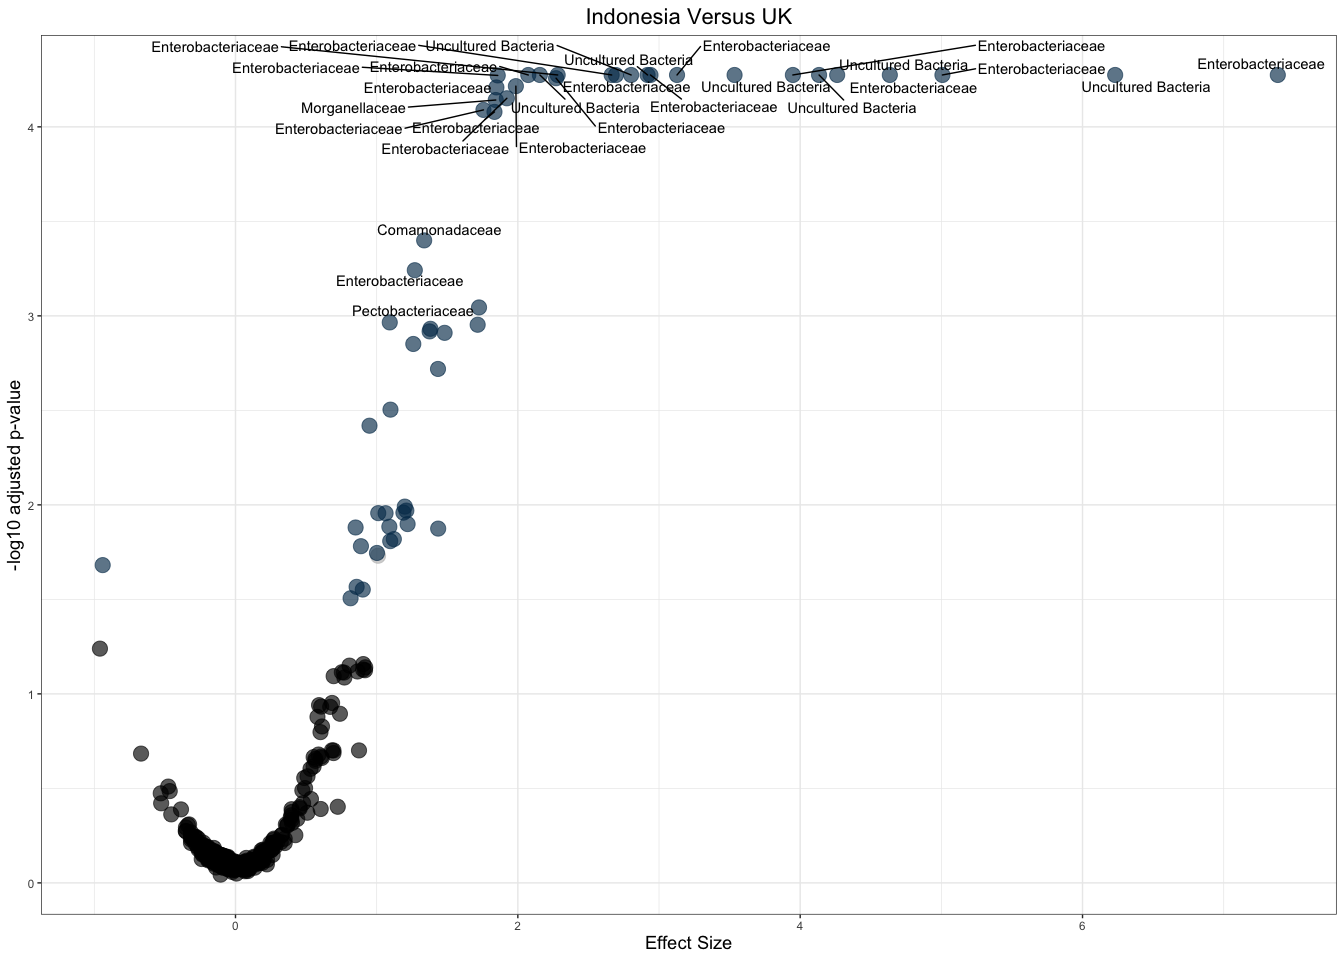
\includegraphics{1.IndonesianVsMaliAndTBControls_CLRMethod_files/figure-latex/unnamed-chunk-29-1} \end{center}

Now let's test the hypothesis that the diversity is different between
islands, which is really what we're asking - are the taxa communities
between our groups different? This is holding the assumption that the
populations are part of a shared ecosystem that has similarities in, for
example, pathogen load. We are now estimating the diversity of
island/population being an ecosystem, so we're focusing on the
ecosystem, not just the samples. If we wanted to reproduce this result,
it is better to focus on the populations that the samples come from, not
just the samples themselves.

Let's test this first using the Shannon diversity index.

\begin{Shaded}
\begin{Highlighting}[]
\CommentTok{# test the hypothesis that the diversity is differnet between islands}
\NormalTok{dv_pop_comparison_cov <-}\StringTok{ }\NormalTok{pop_comparison }\OperatorTok
\StringTok{  }\KeywordTok{divnet}\NormalTok{(}\DataTypeTok{X =} \StringTok{"SamplePop"}\NormalTok{, }\DataTypeTok{ncores =} \DecValTok{8}\NormalTok{)}
\end{Highlighting}
\end{Shaded}

\begin{verbatim}
##   |                                                                              |                                                                      |   0%
\end{verbatim}

\begin{verbatim}
## Warning in MCmat(Y = Y_p, W = W, eY = eY, N = N, Q = Q, base = base, sigma =
## sigma, : Running in series; one of the packages doParallel, foreach or doSNOW is
## missing
\end{verbatim}

\begin{verbatim}
##   |                                                                              |============                                                          |  17%
\end{verbatim}

\begin{verbatim}
## Warning in MCmat(Y = Y_p, W = W, eY = eY, N = N, Q = Q, base = base, sigma =
## sigma, : Running in series; one of the packages doParallel, foreach or doSNOW is
## missing
\end{verbatim}

\begin{verbatim}
##   |                                                                              |=======================                                               |  33%
\end{verbatim}

\begin{verbatim}
## Warning in MCmat(Y = Y_p, W = W, eY = eY, N = N, Q = Q, base = base, sigma =
## sigma, : Running in series; one of the packages doParallel, foreach or doSNOW is
## missing
\end{verbatim}

\begin{verbatim}
##   |                                                                              |===================================                                   |  50%
\end{verbatim}

\begin{verbatim}
## Warning in MCmat(Y = Y_p, W = W, eY = eY, N = N, Q = Q, base = base, sigma =
## sigma, : Running in series; one of the packages doParallel, foreach or doSNOW is
## missing
\end{verbatim}

\begin{verbatim}
##   |                                                                              |===============================================                       |  67%
\end{verbatim}

\begin{verbatim}
## Warning in MCmat(Y = Y_p, W = W, eY = eY, N = N, Q = Q, base = base, sigma =
## sigma, : Running in series; one of the packages doParallel, foreach or doSNOW is
## missing
\end{verbatim}

\begin{verbatim}
##   |                                                                              |==========================================================            |  83%
\end{verbatim}

\begin{verbatim}
## Warning in MCmat(Y = Y_p, W = W, eY = eY, N = N, Q = Q, base = base, sigma =
## sigma, : Running in series; one of the packages doParallel, foreach or doSNOW is
## missing
\end{verbatim}

\begin{verbatim}
##   |                                                                              |======================================================================| 100%
##   |                                                                              |                                                                      |   0%
\end{verbatim}

\begin{verbatim}
## Warning in MCmat(Y = Y_p, W = W, eY = eY, N = N, Q = Q, base = base, sigma =
## sigma, : Running in series; one of the packages doParallel, foreach or doSNOW is
## missing
\end{verbatim}

\begin{verbatim}
##   |                                                                              |============                                                          |  17%
\end{verbatim}

\begin{verbatim}
## Warning in MCmat(Y = Y_p, W = W, eY = eY, N = N, Q = Q, base = base, sigma =
## sigma, : Running in series; one of the packages doParallel, foreach or doSNOW is
## missing
\end{verbatim}

\begin{verbatim}
##   |                                                                              |=======================                                               |  33%
\end{verbatim}

\begin{verbatim}
## Warning in MCmat(Y = Y_p, W = W, eY = eY, N = N, Q = Q, base = base, sigma =
## sigma, : Running in series; one of the packages doParallel, foreach or doSNOW is
## missing
\end{verbatim}

\begin{verbatim}
##   |                                                                              |===================================                                   |  50%
\end{verbatim}

\begin{verbatim}
## Warning in MCmat(Y = Y_p, W = W, eY = eY, N = N, Q = Q, base = base, sigma =
## sigma, : Running in series; one of the packages doParallel, foreach or doSNOW is
## missing
\end{verbatim}

\begin{verbatim}
##   |                                                                              |===============================================                       |  67%
\end{verbatim}

\begin{verbatim}
## Warning in MCmat(Y = Y_p, W = W, eY = eY, N = N, Q = Q, base = base, sigma =
## sigma, : Running in series; one of the packages doParallel, foreach or doSNOW is
## missing
\end{verbatim}

\begin{verbatim}
##   |                                                                              |==========================================================            |  83%
\end{verbatim}

\begin{verbatim}
## Warning in MCmat(Y = Y_p, W = W, eY = eY, N = N, Q = Q, base = base, sigma =
## sigma, : Running in series; one of the packages doParallel, foreach or doSNOW is
## missing
\end{verbatim}

\begin{verbatim}
##   |                                                                              |======================================================================| 100%
##   |                                                                              |                                                                      |   0%
\end{verbatim}

\begin{verbatim}
## Warning in MCmat(Y = Y_p, W = W, eY = eY, N = N, Q = Q, base = base, sigma =
## sigma, : Running in series; one of the packages doParallel, foreach or doSNOW is
## missing
\end{verbatim}

\begin{verbatim}
##   |                                                                              |============                                                          |  17%
\end{verbatim}

\begin{verbatim}
## Warning in MCmat(Y = Y_p, W = W, eY = eY, N = N, Q = Q, base = base, sigma =
## sigma, : Running in series; one of the packages doParallel, foreach or doSNOW is
## missing
\end{verbatim}

\begin{verbatim}
##   |                                                                              |=======================                                               |  33%
\end{verbatim}

\begin{verbatim}
## Warning in MCmat(Y = Y_p, W = W, eY = eY, N = N, Q = Q, base = base, sigma =
## sigma, : Running in series; one of the packages doParallel, foreach or doSNOW is
## missing
\end{verbatim}

\begin{verbatim}
##   |                                                                              |===================================                                   |  50%
\end{verbatim}

\begin{verbatim}
## Warning in MCmat(Y = Y_p, W = W, eY = eY, N = N, Q = Q, base = base, sigma =
## sigma, : Running in series; one of the packages doParallel, foreach or doSNOW is
## missing
\end{verbatim}

\begin{verbatim}
##   |                                                                              |===============================================                       |  67%
\end{verbatim}

\begin{verbatim}
## Warning in MCmat(Y = Y_p, W = W, eY = eY, N = N, Q = Q, base = base, sigma =
## sigma, : Running in series; one of the packages doParallel, foreach or doSNOW is
## missing
\end{verbatim}

\begin{verbatim}
##   |                                                                              |==========================================================            |  83%
\end{verbatim}

\begin{verbatim}
## Warning in MCmat(Y = Y_p, W = W, eY = eY, N = N, Q = Q, base = base, sigma =
## sigma, : Running in series; one of the packages doParallel, foreach or doSNOW is
## missing
\end{verbatim}

\begin{verbatim}
##   |                                                                              |======================================================================| 100%
##   |                                                                              |                                                                      |   0%
\end{verbatim}

\begin{verbatim}
## Warning in MCmat(Y = Y_p, W = W, eY = eY, N = N, Q = Q, base = base, sigma =
## sigma, : Running in series; one of the packages doParallel, foreach or doSNOW is
## missing
\end{verbatim}

\begin{verbatim}
##   |                                                                              |============                                                          |  17%
\end{verbatim}

\begin{verbatim}
## Warning in MCmat(Y = Y_p, W = W, eY = eY, N = N, Q = Q, base = base, sigma =
## sigma, : Running in series; one of the packages doParallel, foreach or doSNOW is
## missing
\end{verbatim}

\begin{verbatim}
##   |                                                                              |=======================                                               |  33%
\end{verbatim}

\begin{verbatim}
## Warning in MCmat(Y = Y_p, W = W, eY = eY, N = N, Q = Q, base = base, sigma =
## sigma, : Running in series; one of the packages doParallel, foreach or doSNOW is
## missing
\end{verbatim}

\begin{verbatim}
##   |                                                                              |===================================                                   |  50%
\end{verbatim}

\begin{verbatim}
## Warning in MCmat(Y = Y_p, W = W, eY = eY, N = N, Q = Q, base = base, sigma =
## sigma, : Running in series; one of the packages doParallel, foreach or doSNOW is
## missing
\end{verbatim}

\begin{verbatim}
##   |                                                                              |===============================================                       |  67%
\end{verbatim}

\begin{verbatim}
## Warning in MCmat(Y = Y_p, W = W, eY = eY, N = N, Q = Q, base = base, sigma =
## sigma, : Running in series; one of the packages doParallel, foreach or doSNOW is
## missing
\end{verbatim}

\begin{verbatim}
##   |                                                                              |==========================================================            |  83%
\end{verbatim}

\begin{verbatim}
## Warning in MCmat(Y = Y_p, W = W, eY = eY, N = N, Q = Q, base = base, sigma =
## sigma, : Running in series; one of the packages doParallel, foreach or doSNOW is
## missing
\end{verbatim}

\begin{verbatim}
##   |                                                                              |======================================================================| 100%
##   |                                                                              |                                                                      |   0%
\end{verbatim}

\begin{verbatim}
## Warning in MCmat(Y = Y_p, W = W, eY = eY, N = N, Q = Q, base = base, sigma =
## sigma, : Running in series; one of the packages doParallel, foreach or doSNOW is
## missing
\end{verbatim}

\begin{verbatim}
##   |                                                                              |============                                                          |  17%
\end{verbatim}

\begin{verbatim}
## Warning in MCmat(Y = Y_p, W = W, eY = eY, N = N, Q = Q, base = base, sigma =
## sigma, : Running in series; one of the packages doParallel, foreach or doSNOW is
## missing
\end{verbatim}

\begin{verbatim}
##   |                                                                              |=======================                                               |  33%
\end{verbatim}

\begin{verbatim}
## Warning in MCmat(Y = Y_p, W = W, eY = eY, N = N, Q = Q, base = base, sigma =
## sigma, : Running in series; one of the packages doParallel, foreach or doSNOW is
## missing
\end{verbatim}

\begin{verbatim}
##   |                                                                              |===================================                                   |  50%
\end{verbatim}

\begin{verbatim}
## Warning in MCmat(Y = Y_p, W = W, eY = eY, N = N, Q = Q, base = base, sigma =
## sigma, : Running in series; one of the packages doParallel, foreach or doSNOW is
## missing
\end{verbatim}

\begin{verbatim}
##   |                                                                              |===============================================                       |  67%
\end{verbatim}

\begin{verbatim}
## Warning in MCmat(Y = Y_p, W = W, eY = eY, N = N, Q = Q, base = base, sigma =
## sigma, : Running in series; one of the packages doParallel, foreach or doSNOW is
## missing
\end{verbatim}

\begin{verbatim}
##   |                                                                              |==========================================================            |  83%
\end{verbatim}

\begin{verbatim}
## Warning in MCmat(Y = Y_p, W = W, eY = eY, N = N, Q = Q, base = base, sigma =
## sigma, : Running in series; one of the packages doParallel, foreach or doSNOW is
## missing
\end{verbatim}

\begin{verbatim}
##   |                                                                              |======================================================================| 100%
##   |                                                                              |                                                                      |   0%
\end{verbatim}

\begin{verbatim}
## Warning in MCmat(Y = Y_p, W = W, eY = eY, N = N, Q = Q, base = base, sigma =
## sigma, : Running in series; one of the packages doParallel, foreach or doSNOW is
## missing
\end{verbatim}

\begin{verbatim}
##   |                                                                              |============                                                          |  17%
\end{verbatim}

\begin{verbatim}
## Warning in MCmat(Y = Y_p, W = W, eY = eY, N = N, Q = Q, base = base, sigma =
## sigma, : Running in series; one of the packages doParallel, foreach or doSNOW is
## missing
\end{verbatim}

\begin{verbatim}
##   |                                                                              |=======================                                               |  33%
\end{verbatim}

\begin{verbatim}
## Warning in MCmat(Y = Y_p, W = W, eY = eY, N = N, Q = Q, base = base, sigma =
## sigma, : Running in series; one of the packages doParallel, foreach or doSNOW is
## missing
\end{verbatim}

\begin{verbatim}
##   |                                                                              |===================================                                   |  50%
\end{verbatim}

\begin{verbatim}
## Warning in MCmat(Y = Y_p, W = W, eY = eY, N = N, Q = Q, base = base, sigma =
## sigma, : Running in series; one of the packages doParallel, foreach or doSNOW is
## missing
\end{verbatim}

\begin{verbatim}
##   |                                                                              |===============================================                       |  67%
\end{verbatim}

\begin{verbatim}
## Warning in MCmat(Y = Y_p, W = W, eY = eY, N = N, Q = Q, base = base, sigma =
## sigma, : Running in series; one of the packages doParallel, foreach or doSNOW is
## missing
\end{verbatim}

\begin{verbatim}
##   |                                                                              |==========================================================            |  83%
\end{verbatim}

\begin{verbatim}
## Warning in MCmat(Y = Y_p, W = W, eY = eY, N = N, Q = Q, base = base, sigma =
## sigma, : Running in series; one of the packages doParallel, foreach or doSNOW is
## missing
\end{verbatim}

\begin{verbatim}
##   |                                                                              |======================================================================| 100%
\end{verbatim}

\begin{Shaded}
\begin{Highlighting}[]
\CommentTok{# Plot the results for each individual}
\KeywordTok{plot}\NormalTok{(dv_pop_comparison_cov}\OperatorTok{$}\NormalTok{shannon, pop_comparison, }\DataTypeTok{col =} \StringTok{"SamplePop"}\NormalTok{) }\OperatorTok{+}\StringTok{ }\KeywordTok{scale_colour_manual}\NormalTok{(}\DataTypeTok{values=}\KeywordTok{c}\NormalTok{(IndonesiaCol,MaliCol,UKCol))}
\end{Highlighting}
\end{Shaded}

\begin{center}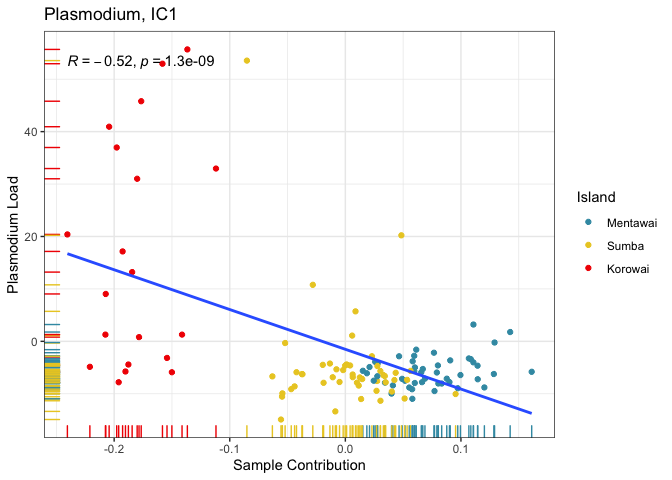
\includegraphics{1.IndonesianVsMaliAndTBControls_CLRMethod_files/figure-latex/unnamed-chunk-30-1} \end{center}

We can see that, as a population, the Malian samples have the highest
diversity, followed by the Indonesian samples, then the UK samples.

Let's test this hypothesis formally.

\begin{Shaded}
\begin{Highlighting}[]
\CommentTok{# test that these populations are actually different}
\KeywordTok{testDiversity}\NormalTok{(dv_pop_comparison_cov, }\StringTok{"shannon"}\NormalTok{)}
\end{Highlighting}
\end{Shaded}

\begin{verbatim}
## Hypothesis testing:
##   p-value for global test: 0
\end{verbatim}

\begin{verbatim}
##                 Estimates Standard Errors p-values
## (Intercept)     0.9115722     0.001925960        0
## predictorsMali  0.6930572     0.009926869        0
## predictorsUK   -0.3736744     0.020806487        0
\end{verbatim}

The result tells us that the mean Shannon diversity in the Indonesian
population at the Phylum-level is 0.92, and it is significantly higher
by 0.76 orders, on average, in the Malian population. We can also see
that the UK population is significantly lower than the Indonesian
population by 0.38 orders, on average.

Let's do the same thing for Simpson diversity.

\begin{Shaded}
\begin{Highlighting}[]
\KeywordTok{plot}\NormalTok{(dv_pop_comparison_cov}\OperatorTok{$}\NormalTok{simpson, pop_comparison, }\DataTypeTok{col =} \StringTok{"SamplePop"}\NormalTok{) }\OperatorTok{+}\StringTok{ }\KeywordTok{scale_colour_manual}\NormalTok{(}\DataTypeTok{values=}\KeywordTok{c}\NormalTok{(IndonesiaCol,MaliCol,UKCol))}
\end{Highlighting}
\end{Shaded}

\begin{center}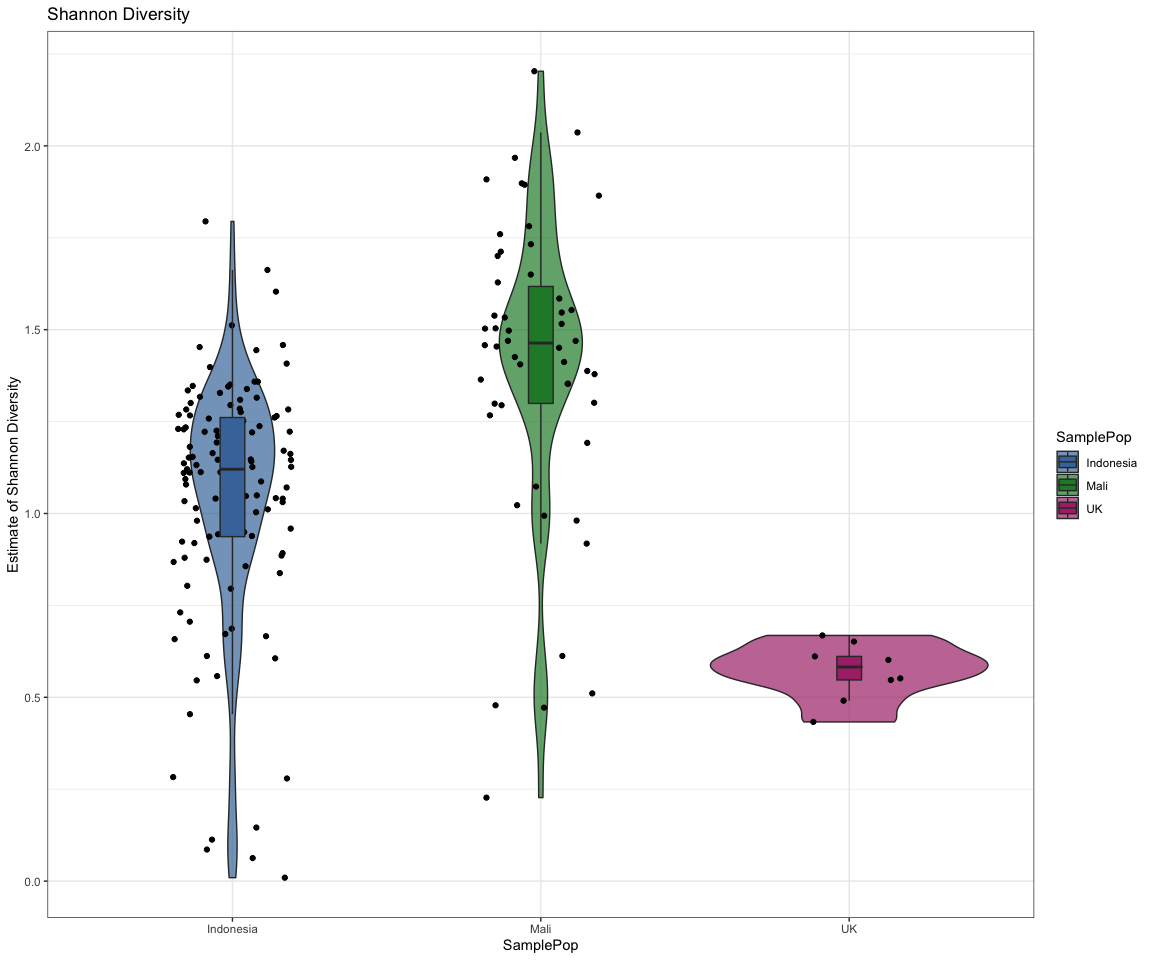
\includegraphics{1.IndonesianVsMaliAndTBControls_CLRMethod_files/figure-latex/unnamed-chunk-32-1} \end{center}

With the Simpson index, the same trend seems to hold at the
population-level: the UK population has the highest Simpson index (i.e.,
lowest diversity), followed by the Indonesian population, then the
Malian population.

Again, let's test this formally.

\begin{Shaded}
\begin{Highlighting}[]
\KeywordTok{testDiversity}\NormalTok{(dv_pop_comparison_cov, }\StringTok{"simpson"}\NormalTok{)}
\end{Highlighting}
\end{Shaded}

\begin{verbatim}
## Hypothesis testing:
##   p-value for global test: 0
\end{verbatim}

\begin{verbatim}
##                  Estimates Standard Errors p-values
## (Intercept)     0.59490753     0.001286851        0
## predictorsMali -0.35013171     0.004050794        0
## predictorsUK    0.07074015     0.019510844        0
\end{verbatim}

The result tells us that the mean Simpson diversity index in the
Indonesian population at the Phylum-level is 0.59, and it is
significantly lower by 0.36 orders, on average, in the Malian
population. We can also see that the UK population is significantly
higher than the Indonesian population by 0.07 orders, on average.

\hypertarget{beta-diversity}{%
\section{Beta Diversity}\label{beta-diversity}}

Beta diversity is a measure of dissimilarity metric between samples to
compare differneces in species composition. It's helpful to know not
only how taxonomically/pathogenically rich each sample is, but also to
see differences in samples and populations.

There are multiple beta diversity measures to use, including Bray-curtis
dissimilarity (based on abundances), Jaccard distance (based on presence
or absence), Euclidean distance, and Unifrac (based on sequence
distances using a phylogenetic tree).

The Bray--Curtis dissimilarity metric is probably the most popular beta
diversity metric and is bounded between 0 and 1, where 0 means the two
sites have the same composition (all species are shared), and 1 means
the two sites do not share any species.

Unlike alpha diversity, beta diversity is not as sensitive to
singletons, and it has even been suggested that `using simple
proportions' (i.e., relative abundance) on non-rarefied data
\href{https://github.com/joey711/phyloseq/issues/470}{is fine}. I
haven't found enough information on this one way or another (it seems
like people are far more opinionated on alpha diversity than beta
diversity), but regardless, let's try it out a few different methods.
First we'll try out Bray-curtis dissimilarity and Jaccard distances on
the relative abundances using phyloseq, then we'll use the Bray-curtis
dissimilarity and Euclidean beta diversity metrics from DivNet (these
are the only two that are available in DivNet).

First, let's test the Phyloseq method using Bray-curtis dissimilarity
and Jaccard.

\begin{Shaded}
\begin{Highlighting}[]
\CommentTok{# Change counts to relative abundances}
\NormalTok{ps4.rel <-}\StringTok{ }\NormalTok{microbiome}\OperatorTok{::}\KeywordTok{transform}\NormalTok{(merged_phylo_counts_withSingletons, }\StringTok{"compositional"}\NormalTok{)}
\CommentTok{# calculat Bray-curtis dissimilarity}
\NormalTok{bx.ord_pcoa_bray <-}\StringTok{ }\KeywordTok{ordinate}\NormalTok{(ps4.rel, }\StringTok{"PCoA"}\NormalTok{, }\StringTok{"bray"}\NormalTok{)}

\CommentTok{# Make an ordination plot using bray's dissimilarity metric}
\NormalTok{beta.ps1 <-}\StringTok{ }\KeywordTok{plot_ordination}\NormalTok{(ps4.rel, }
\NormalTok{                            bx.ord_pcoa_bray, }
                            \DataTypeTok{color=}\StringTok{"SamplePop"}\NormalTok{, }
                            \DataTypeTok{label =} \StringTok{"SampleName"}\NormalTok{) }\OperatorTok{+}\StringTok{ }
\StringTok{  }\KeywordTok{geom_point}\NormalTok{(}\KeywordTok{aes}\NormalTok{(), }\DataTypeTok{size=} \DecValTok{4}\NormalTok{) }\OperatorTok{+}\StringTok{ }
\StringTok{  }\KeywordTok{theme}\NormalTok{(}\DataTypeTok{plot.title =} \KeywordTok{element_text}\NormalTok{(}\DataTypeTok{hjust =} \DecValTok{0}\NormalTok{, }\DataTypeTok{size =} \DecValTok{12}\NormalTok{))}

\CommentTok{# add in an ellipse}
\NormalTok{beta.ps1 }\OperatorTok{+}\StringTok{ }\KeywordTok{stat_ellipse}\NormalTok{() }\OperatorTok{+}\StringTok{ }\KeywordTok{theme_bw}\NormalTok{(}\DataTypeTok{base_size =} \DecValTok{14}\NormalTok{) }\OperatorTok{+}\StringTok{ }
\StringTok{  }\KeywordTok{theme}\NormalTok{(}\DataTypeTok{panel.grid.major =} \KeywordTok{element_blank}\NormalTok{(), }\DataTypeTok{panel.grid.minor =} \KeywordTok{element_blank}\NormalTok{()) }\OperatorTok{+}
\StringTok{  }\KeywordTok{scale_colour_manual}\NormalTok{(}\DataTypeTok{values=}\KeywordTok{c}\NormalTok{(IndonesiaCol,MaliCol,UKCol))}
\end{Highlighting}
\end{Shaded}

\begin{center}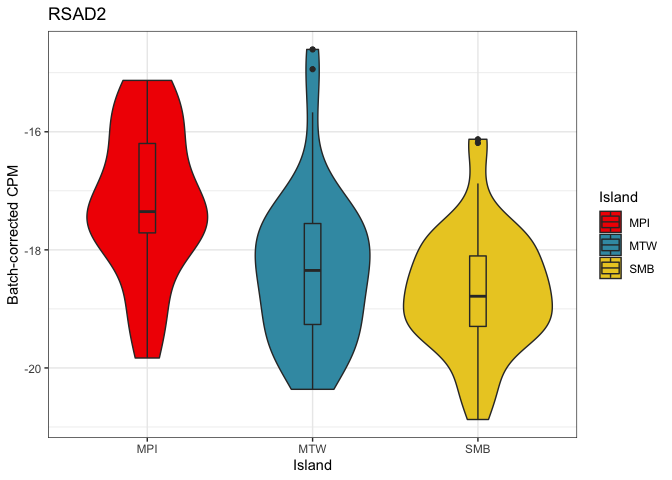
\includegraphics{1.IndonesianVsMaliAndTBControls_CLRMethod_files/figure-latex/unnamed-chunk-34-1} \end{center}

\begin{Shaded}
\begin{Highlighting}[]
\CommentTok{# Change counts to relative abundances}
\NormalTok{ps4.rel <-}\StringTok{ }\NormalTok{microbiome}\OperatorTok{::}\KeywordTok{transform}\NormalTok{(merged_phylo_counts_withSingletons, }\StringTok{"compositional"}\NormalTok{)}
\CommentTok{# calculat Bray-curtis dissimilarity}
\NormalTok{bx.ord_pcoa_jaccard <-}\StringTok{ }\KeywordTok{ordinate}\NormalTok{(ps4.rel, }\StringTok{"PCoA"}\NormalTok{, }\StringTok{"jaccard"}\NormalTok{)}

\CommentTok{# Make an ordination plot using bray's dissimilarity metric}
\NormalTok{beta.ps1 <-}\StringTok{ }\KeywordTok{plot_ordination}\NormalTok{(ps4.rel, }
\NormalTok{                            bx.ord_pcoa_jaccard, }
                            \DataTypeTok{color=}\StringTok{"SamplePop"}\NormalTok{, }
                            \DataTypeTok{label =} \StringTok{"SampleName"}\NormalTok{) }\OperatorTok{+}\StringTok{ }
\StringTok{  }\KeywordTok{geom_point}\NormalTok{(}\KeywordTok{aes}\NormalTok{(), }\DataTypeTok{size=} \DecValTok{4}\NormalTok{) }\OperatorTok{+}\StringTok{ }
\StringTok{  }\KeywordTok{theme}\NormalTok{(}\DataTypeTok{plot.title =} \KeywordTok{element_text}\NormalTok{(}\DataTypeTok{hjust =} \DecValTok{0}\NormalTok{, }\DataTypeTok{size =} \DecValTok{12}\NormalTok{))}

\CommentTok{# add in an ellipse}
\NormalTok{beta.ps1 }\OperatorTok{+}\StringTok{ }\KeywordTok{stat_ellipse}\NormalTok{() }\OperatorTok{+}\StringTok{ }\KeywordTok{theme_bw}\NormalTok{(}\DataTypeTok{base_size =} \DecValTok{14}\NormalTok{) }\OperatorTok{+}\StringTok{ }
\StringTok{  }\KeywordTok{theme}\NormalTok{(}\DataTypeTok{panel.grid.major =} \KeywordTok{element_blank}\NormalTok{(), }\DataTypeTok{panel.grid.minor =} \KeywordTok{element_blank}\NormalTok{()) }\OperatorTok{+}
\StringTok{  }\KeywordTok{scale_colour_manual}\NormalTok{(}\DataTypeTok{values=}\KeywordTok{c}\NormalTok{(IndonesiaCol,MaliCol,UKCol))}
\end{Highlighting}
\end{Shaded}

\begin{verbatim}
## Warning in MASS::cov.trob(data[, vars]): Probable convergence failure
\end{verbatim}

\begin{center}\includegraphics{1.IndonesianVsMaliAndTBControls_CLRMethod_files/figure-latex/unnamed-chunk-34-2} \end{center}

For both estimates, we can see that the Malian data is the least similar
from the Indonesian and UK data. We can also see that some samples,
particularly those with higher Plasmodium load, cluster closer to the
Malian samples.

Now let's use our results from DivNet, which corrects for sequencing
depth, and see how this compares.

For the first bray-curtis dissimilarity analysis, we'll look at all of
our samples individually, then we'll look at how bray-curtis
dissimilarity looks like between islands (with hypothesis testing).

\begin{Shaded}
\begin{Highlighting}[]
\CommentTok{# First, let's look at Bray-curtis dissimilarity at the individual sample level}
\NormalTok{bray_est <-}\StringTok{ }\KeywordTok{simplifyBeta}\NormalTok{(dv_pop_comparison, pop_comparison, }\StringTok{"bray-curtis"}\NormalTok{, }\StringTok{"SamplePop"}\NormalTok{)}

\CommentTok{# add in group comparisons and plot}
\NormalTok{bray_est}\OperatorTok{$}\NormalTok{group=}\KeywordTok{paste}\NormalTok{(bray_est}\OperatorTok{$}\NormalTok{Covar1,bray_est}\OperatorTok{$}\NormalTok{Covar2,}\DataTypeTok{sep=}\StringTok{"_"}\NormalTok{)}
\KeywordTok{ggplot}\NormalTok{(bray_est, }\KeywordTok{aes}\NormalTok{(}\DataTypeTok{x =} \KeywordTok{interaction}\NormalTok{(Covar1, Covar2), }\DataTypeTok{y =}\NormalTok{ beta_est, }\DataTypeTok{fill=}\NormalTok{group)) }\OperatorTok{+}
\StringTok{  }\KeywordTok{geom_violin}\NormalTok{(}\DataTypeTok{alpha=}\FloatTok{0.7}\NormalTok{) }\OperatorTok{+}\StringTok{ }\KeywordTok{geom_boxplot}\NormalTok{(}\DataTypeTok{width=}\FloatTok{0.1}\NormalTok{) }\OperatorTok{+}\StringTok{ }\KeywordTok{xlab}\NormalTok{(}\StringTok{"Population Comparisons"}\NormalTok{) }\OperatorTok{+}\StringTok{ }
\StringTok{  }\KeywordTok{theme}\NormalTok{(}\DataTypeTok{legend.position=}\StringTok{"none"}\NormalTok{) }\OperatorTok{+}\StringTok{ }\KeywordTok{ggtitle}\NormalTok{(}\StringTok{"Bray-Curtis Distance Estimate"}\NormalTok{) }\OperatorTok{+}
\StringTok{  }\KeywordTok{ylab}\NormalTok{(}\StringTok{"Bray-Curtis Distance"}\NormalTok{)}
\end{Highlighting}
\end{Shaded}

\begin{center}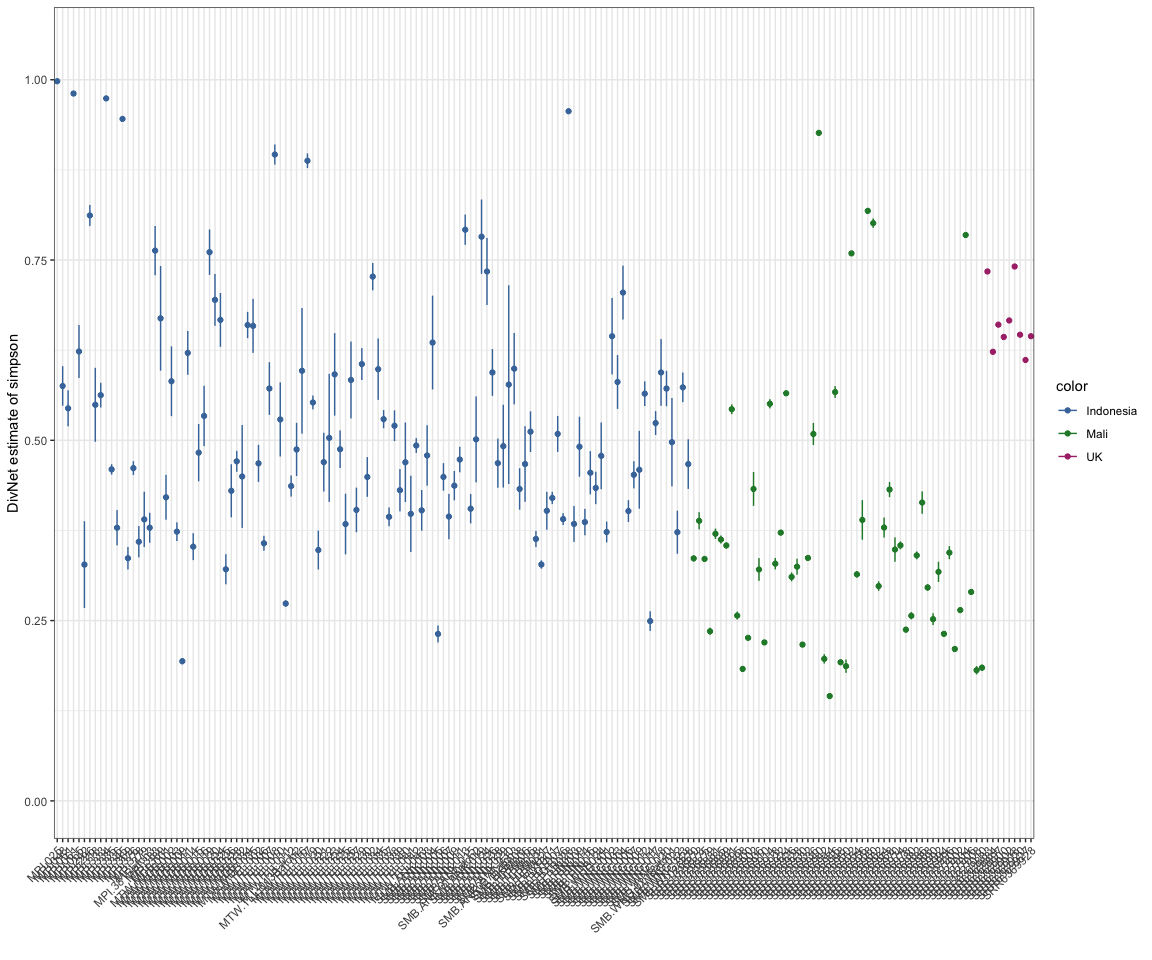
\includegraphics{1.IndonesianVsMaliAndTBControls_CLRMethod_files/figure-latex/unnamed-chunk-35-1} \end{center}

From DivNet, again we can see that the greatest dissimilarity is between
the Malian population. Unsurpiringly, the least dissimilar samples are
comparing UK samples to UK samples and Indonesian samples to Indonesian
samples, however this isn't the case for the Malian samples - we can see
that the mean Malian Bray-Curtis dissimilarity estimate is nearly 0.5,
which is even higher than comparing UK samples to Indonesian samples. We
also see quite a but of spread in distance estimates within Indonesia,
but in the UK, they seem to be relatively similar to one another.

Now let's test beta diversity in DivNet using Euclidean distance.

\begin{Shaded}
\begin{Highlighting}[]
\CommentTok{# First, let's look at Bray-curtis dissimilarity at the individual sample level}
\NormalTok{bray_est_eucl <-}\StringTok{ }\KeywordTok{simplifyBeta}\NormalTok{(dv_pop_comparison, pop_comparison, }\StringTok{"euclidean"}\NormalTok{, }\StringTok{"SamplePop"}\NormalTok{)}

\CommentTok{# add in group comparisons and plot}
\NormalTok{bray_est_eucl}\OperatorTok{$}\NormalTok{group <-}\StringTok{ }\KeywordTok{paste}\NormalTok{(bray_est_eucl}\OperatorTok{$}\NormalTok{Covar1, bray_est_eucl}\OperatorTok{$}\NormalTok{Covar2,}\DataTypeTok{sep=}\StringTok{"_"}\NormalTok{)}

\KeywordTok{ggplot}\NormalTok{(bray_est_eucl, }\KeywordTok{aes}\NormalTok{(}\DataTypeTok{x =} \KeywordTok{interaction}\NormalTok{(Covar1, Covar2), }\DataTypeTok{y =}\NormalTok{ beta_est, }\DataTypeTok{fill=}\NormalTok{group)) }\OperatorTok{+}
\StringTok{  }\KeywordTok{geom_violin}\NormalTok{(}\DataTypeTok{alpha=}\FloatTok{0.7}\NormalTok{) }\OperatorTok{+}\StringTok{ }\KeywordTok{geom_boxplot}\NormalTok{(}\DataTypeTok{width=}\FloatTok{0.1}\NormalTok{) }\OperatorTok{+}\StringTok{ }\KeywordTok{xlab}\NormalTok{(}\StringTok{"Population Comparisons"}\NormalTok{) }\OperatorTok{+}\StringTok{ }
\StringTok{  }\KeywordTok{theme}\NormalTok{(}\DataTypeTok{legend.position=}\StringTok{"none"}\NormalTok{) }\OperatorTok{+}\StringTok{ }\KeywordTok{ggtitle}\NormalTok{(}\StringTok{"Euclidean Distance Estimate"}\NormalTok{) }\OperatorTok{+}
\StringTok{  }\KeywordTok{ylab}\NormalTok{(}\StringTok{"Euclidean Distance"}\NormalTok{)}
\end{Highlighting}
\end{Shaded}

\begin{center}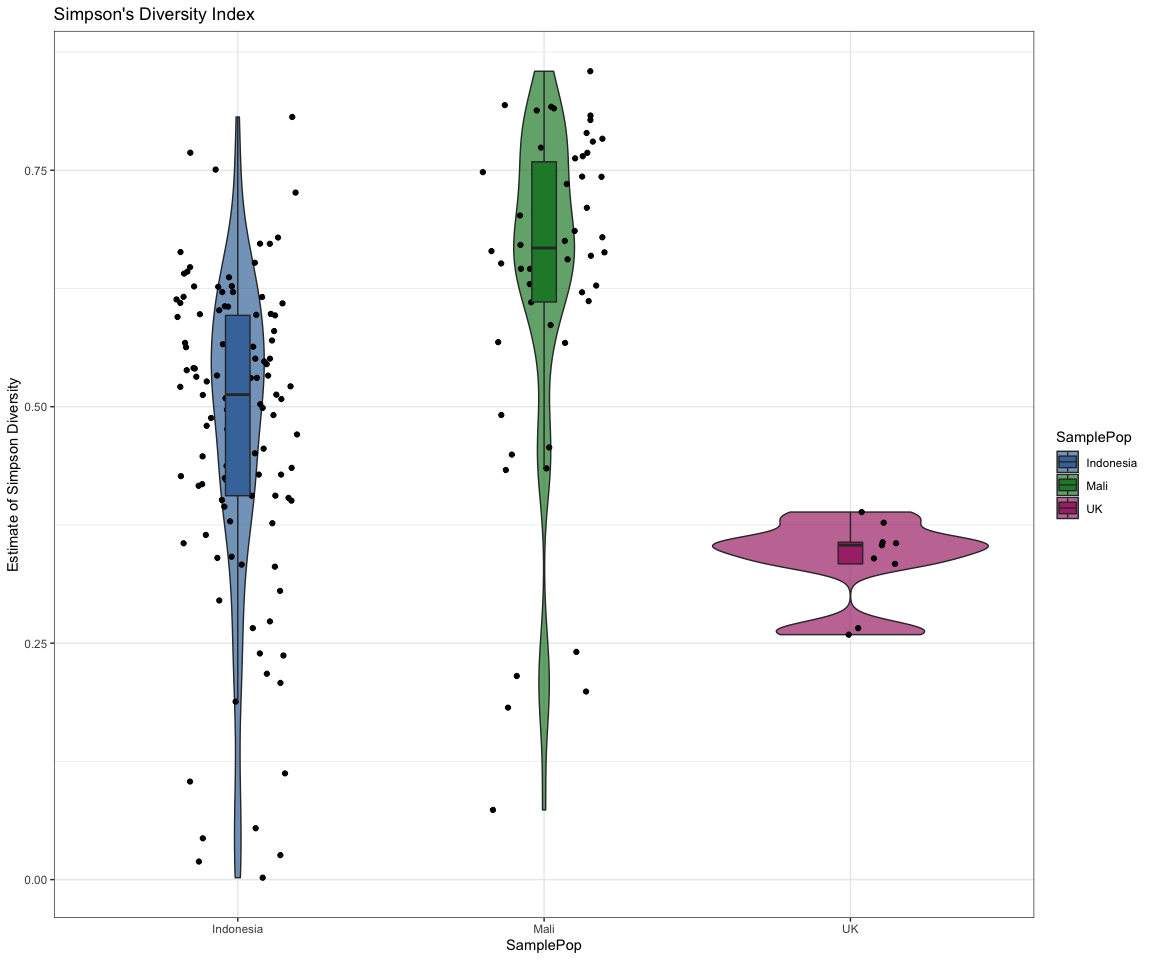
\includegraphics{1.IndonesianVsMaliAndTBControls_CLRMethod_files/figure-latex/unnamed-chunk-36-1} \end{center}

We can see similar trends in using Euclidean distance, compared to the
Bray-Curtis dissimilarity metric.

Now let's see how this looks like for island-level comparisons.

\begin{Shaded}
\begin{Highlighting}[]
\CommentTok{# Bray-Curtis dissimilarity}
\KeywordTok{simplifyBeta}\NormalTok{(dv_pop_comparison_cov, pop_comparison, }\StringTok{"bray-curtis"}\NormalTok{, }\StringTok{"SamplePop"}\NormalTok{) }\OperatorTok
\StringTok{  }\KeywordTok{ggplot}\NormalTok{(}\KeywordTok{aes}\NormalTok{(}\DataTypeTok{x =} \KeywordTok{interaction}\NormalTok{(Covar1, Covar2), }
             \DataTypeTok{y =}\NormalTok{ beta_est)) }\OperatorTok{+}
\StringTok{  }\KeywordTok{geom_point}\NormalTok{() }\OperatorTok{+}
\StringTok{  }\KeywordTok{geom_linerange}\NormalTok{(}\KeywordTok{aes}\NormalTok{(}\DataTypeTok{ymin =}\NormalTok{ lower, }\DataTypeTok{ymax =}\NormalTok{ upper)) }\OperatorTok{+}\StringTok{ }
\StringTok{  }\KeywordTok{theme}\NormalTok{(}\DataTypeTok{axis.text.x =} \KeywordTok{element_text}\NormalTok{(}\DataTypeTok{angle =} \DecValTok{45}\NormalTok{, }\DataTypeTok{hjust =} \DecValTok{1}\NormalTok{)) }\OperatorTok{+}
\StringTok{  }\KeywordTok{xlab}\NormalTok{(}\StringTok{""}\NormalTok{) }\OperatorTok{+}\StringTok{ }\KeywordTok{ylab}\NormalTok{(}\StringTok{"Estimates of Bray-Curtis distance"}\NormalTok{)}
\end{Highlighting}
\end{Shaded}

\begin{center}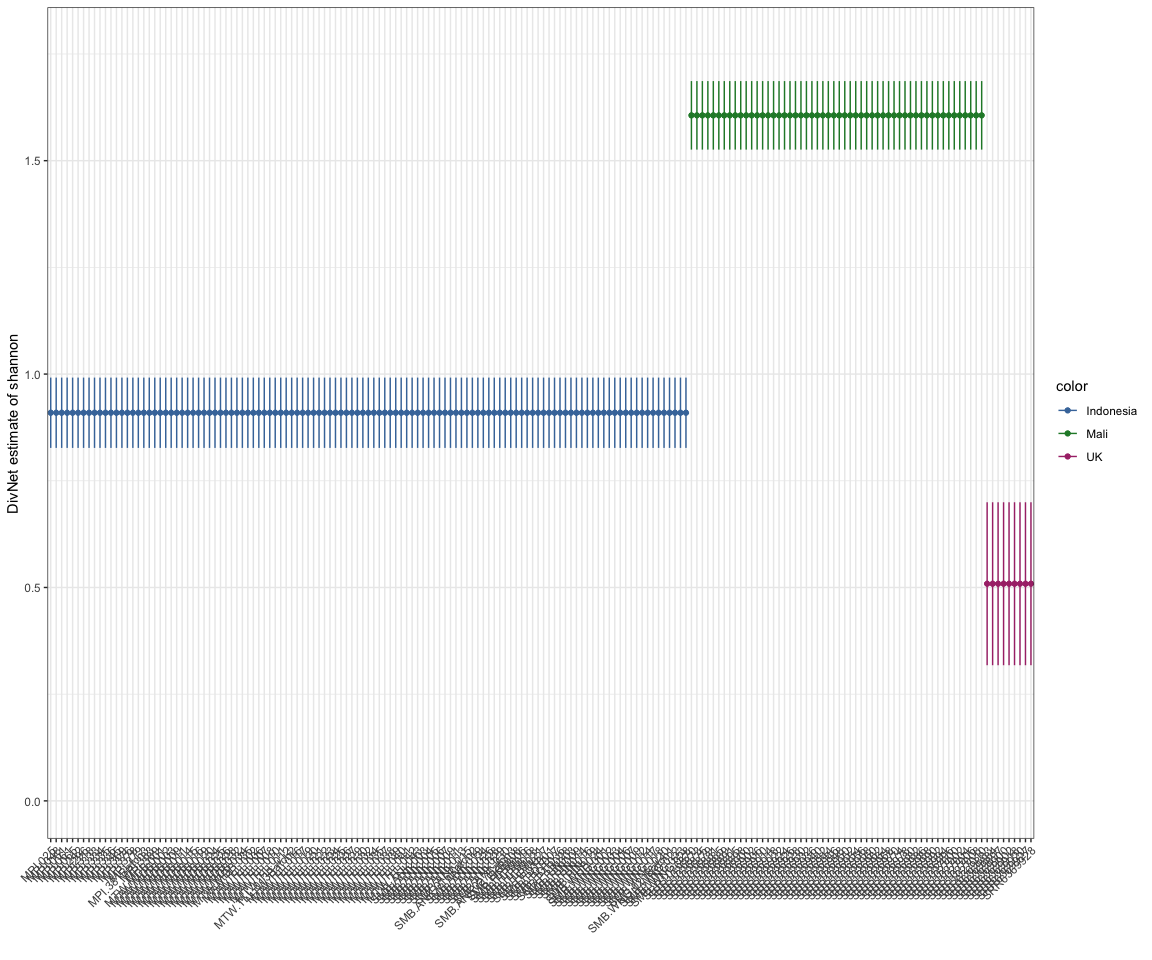
\includegraphics{1.IndonesianVsMaliAndTBControls_CLRMethod_files/figure-latex/unnamed-chunk-37-1} \end{center}

\begin{Shaded}
\begin{Highlighting}[]
\CommentTok{# Euclidean distance}
\KeywordTok{simplifyBeta}\NormalTok{(dv_pop_comparison_cov, pop_comparison, }\StringTok{"euclidean"}\NormalTok{, }\StringTok{"SamplePop"}\NormalTok{) }\OperatorTok
\StringTok{  }\KeywordTok{ggplot}\NormalTok{(}\KeywordTok{aes}\NormalTok{(}\DataTypeTok{x =} \KeywordTok{interaction}\NormalTok{(Covar1, Covar2), }
             \DataTypeTok{y =}\NormalTok{ beta_est)) }\OperatorTok{+}
\StringTok{  }\KeywordTok{geom_point}\NormalTok{() }\OperatorTok{+}
\StringTok{  }\KeywordTok{geom_linerange}\NormalTok{(}\KeywordTok{aes}\NormalTok{(}\DataTypeTok{ymin =}\NormalTok{ lower, }\DataTypeTok{ymax =}\NormalTok{ upper)) }\OperatorTok{+}\StringTok{ }
\StringTok{  }\KeywordTok{theme}\NormalTok{(}\DataTypeTok{axis.text.x =} \KeywordTok{element_text}\NormalTok{(}\DataTypeTok{angle =} \DecValTok{45}\NormalTok{, }\DataTypeTok{hjust =} \DecValTok{1}\NormalTok{)) }\OperatorTok{+}
\StringTok{  }\KeywordTok{xlab}\NormalTok{(}\StringTok{""}\NormalTok{) }\OperatorTok{+}\StringTok{ }\KeywordTok{ylab}\NormalTok{(}\StringTok{"Estimates of Bray-Curtis distance"}\NormalTok{)}
\end{Highlighting}
\end{Shaded}

\begin{center}\includegraphics{1.IndonesianVsMaliAndTBControls_CLRMethod_files/figure-latex/unnamed-chunk-37-2} \end{center}

This confirms that indeeed, the Malian population is the most dissimilar
from the other two populations.

Thanks for sticking through to the end!

\end{document}
